\documentclass[10pt, draft]{book}
\usepackage{graphicx}
\graphicspath{ {./figs/} }
\usepackage{hyperref} % per fare riferimenti ad elementi
\usepackage[T1]{fontenc}
\usepackage{kpfonts}
\usepackage{geometry}
\geometry{a4paper, total = {150mm, 240mm}}
\usepackage[italian]{babel}
\usepackage[utf8]{inputenc}
\usepackage{scrextend} % per addmargin
\usepackage{mathtools, amssymb} % simboli matematici
\usepackage{tabularx} % per tabelle particolari
%%inizio blocco esempio
\usepackage[most]{tcolorbox}
\usepackage{nicefrac}
\usepackage{xcolor}
\definecolor{lyellow}{HTML}{fee9be}
\definecolor{bluegray}{HTML}{dedce6}
\usepackage{float}
\usepackage{makecell}
\setlength{\parindent}{0pt}
\newcommand{\tightlist}{%
\setlength{\itemsep}{1pt}\setlength{\parskip}{0pt}\setlength{\parsep}{0pt}}
\newcounter{example}[section]
\renewcommand\theexample{\thesection.\alph{example}}
\NewDocumentEnvironment{example}{ O{} }
{
    \refstepcounter{example}
    \colorlet{colexam}{black} % Global example color
    \newtcolorbox{examplebox}{%
        % Example Frame Start
        empty,% Empty previously set parameters
        title={Esempio~\theexample: #1},% use \thetcbcounter to access the example counter text
        % Attaching a box requires an overlay
        attach boxed title to top left,
        % Ensures proper line breaking in longer titles
        minipage boxed title,
        % (boxed title style requires an overlay)
        boxed title style={empty,size=minimal,toprule=0pt,top=4pt,left=1em,overlay={}},
        coltitle=colexam,fonttitle=\bfseries,
        before=\par\medskip\noindent,parbox=false,boxsep=0pt,left=3mm,right=0mm,top=2pt,breakable,pad at break=0mm,
        before upper=\csname @totalleftmargin\endcsname0pt, % Use instead of parbox=true. This ensures parskip is inherited by box.
        % Handles box when it exists on one page only
        overlay unbroken={\draw[colexam,line width=.5pt] ([xshift=-0pt]title.north west) -- ([xshift=-0pt]frame.south west); },
        % Handles multipage box: first page
        overlay first={\draw[colexam,line width=.5pt] ([xshift=-0pt]title.north west) -- ([xshift=-0pt]frame.south west); },
        % Handles multipage box: middle page
        overlay middle={\draw[colexam,line width=.5pt] ([xshift=-0pt]frame.north west) -- ([xshift=-0pt]frame.south west); },
        % Handles multipage box: last page
        overlay last={\draw[colexam,line width=.5pt] ([xshift=-0pt]frame.north west) -- ([xshift=-0pt]frame.south west); },%
    }
    \begin{examplebox}
}{
    \end{examplebox}\endlist
}
%%fine blocco esempio
% Autosizing absolute value
\DeclarePairedDelimiter\abs{\lvert}{\rvert}%
\DeclarePairedDelimiter\norm{\lVert}{\rVert}%
% Swap the definition of \abs* and \norm*, so that \abs and \norm resizes the
% size of the brackets, and the starred version does not.
\makeatletter
    \let\oldabs\abs
    \def\abs{\@ifstar{\oldabs}{\oldabs*}}
    %
    \let\oldnorm\norm
    \def\norm{\@ifstar{\oldnorm}{\oldnorm*}}
\makeatother
% fine Autosizing absolute value

\title{\Huge{\textbf{Appunti di biostatistica}}}
\author{\Large{Gaia Di Francescantonio}}
\date{a. a. 2021/2022}

\begin{document}
\maketitle
\tableofcontents

\part{Principi, descrizione ed inferenza}

\chapter{Introduzione alla statistica (B1)} \footnote{Capitolo 1, Whitlock and Schluter, Analisi statistica dei dati biologici (2010)}


\section{Statistica}
I biologi studiano le proprietà degli esseri viventi. Misurare queste proprietà è però un compito assai impegnativo, perché non esistono due individui appartenenti alla stessa popolazione biologica che siano esattamente identici. Inoltre, non siamo quasi mai in grado di misurare ogni individuo presente nella popolazione, e siamo quindi vincolati dal tempo e dai fondi disponibili a limitare le misurazioni a un campione di individui estratto dalla popolazione. Ma il campionamento introduce incertezza. Per effetto del caso, le proprietà del campione non sono uguali a quelle della popolazione dalla quale il campione è stato estratto: le misure ottenute da un campione, infatti, sono influenzate dall'inclusione in quel campione di certi individui piuttosto che altri.
\\
La \textbf{statistica} è una disciplina che permette di descrivere e misurare diversi aspetti della natura basandosi su campioni. Soprattutto, la statistica consente di quantificare l'incertezza di queste misure, ovvero di determinare la probabile entità del loro scostamento dal valore vero. La statistica si occupa del processo di \textbf{stima}, cioè del processo con cui si inferisce (stima) una grandezza incognita di una popolazione usando i \textbf{dati campionari}, ossia i dati provenienti da un campione. Se applicati correttamente, gli strumenti della stima permettono di approssimare pressoché ogni grandezza tipica di una popolazione usando soltanto campioni.
\\
Oltre a stimare grandezze incognite, la statistica permette di valutare le differenze tra gruppi e le relazioni tra variabili.
\\
\\
Tutte le grandezze che descrivono le popolazioni (medie, proporzioni, misure di variazione e misure di relazione) sono dette \textbf{parametri}. La statistica dice come si possono stimare nel modo migliore i parametri usando delle misurazioni relative a un campione. Il parametro è quindi il valore vero e la stima (il risultato del processo di stima) è un'approssimazione del valore vero, soggetta a errore. Se fossimo in grado di misurare ogni membro della popolazione, potremmo conoscere il parametro senza errore, ma ciò è possibile solo molto raramente. Invece, si utilizzano stime su dati incompleti per approssimare questo valore vero. Disponendo di strumenti statistici appropriati, siamo in grado di determinare la bontà delle approssimazioni.
\\
\\
La statistica si occupa anche della verifica delle ipotesi (o test delle ipotesi).
\\
\\
La statistica prevede il susseguirsi di alcuni passaggi standard: raccogliere, organizzare, visualizzare, analizzare, interpretare e presentare dati.

\section{Popolazione}
La capacità di ottenere misure affidabili delle caratteristiche delle popolazioni e di valutare l'incertezza di queste misure dipende in modo critico da come si campionano le popolazioni stesse.
\\
Il primo passo nella raccolta di dati biologici di qualsiasi tipo è decidere quale sia la popolazione da campionare. Una \textbf{popolazione statistica} è l'intero insieme di individui o di unità che interessano a un ricercatore e della quale si vogliono conoscere i parametri. Di solito una popolazione è costituita da un grande numero di individui; nella maggior parte dei casi, si suppone in effetti che la popolazione sia infinitamente grande.
\\
Le caratteristiche che si misurano in tale gruppo di elementi devono essere necessariamente variabili (altrimenti la misurazione sarebbe inutile).
\\
Si deve essere in grado di identificare un sistema e di identificarne delle caratteristiche, misurare queste caratteristiche ed operare un'inferenza che permetta di estrapolare le informazioni misurate all'intera \textbf{popolazione biologica} (che può coincidere con la popolazione statistica, ma il più delle volte non è così).

\section{Campione e stima}
Un \textbf{campione statistico} è invece un insieme molto più piccolo di individui selezionati dalla popolazione statistica. Il ricercatore impiega il campione per trarre conclusioni che siano possibilmente valide per l'intera popolazione. 
\\
Il campione serve per stimare una caratteristica e la sua variabilità nella popolazione.
\\
Si ricorre alla stima quando non è possibile effettuare la misurazione del parametro su tutti gli elementi della popolazione statistica.
\\
\\
Spesso, l'\textbf{unità statistica} di base del campionamento è il singolo individuo. Talvolta, però, l'unità fondamentale di uno studio è un gruppo di individui, nel qual caso un campione è costituito da un sottoinsieme di tali unità. 
\\
Un'\textbf{unità campionaria} è il soggetto/individuo/evento/caso/osservazione/ecc. su cui si compiono le misurazioni delle variabili. Il concetto di unità statistica ha un valore più ampio, mentre l'unità campionaria è uno degli elementi che compongono il campione, selezionati all'interno della popolazione statistica.
\\
Per designare l'unità di campionamento gli scienziati impiegano diversi termini, quali "unità", "individuo", "soggetto" o "replica".
\\
\\
Il campione deve essere:
\begin{itemize} \tightlist
    \item \textbf{rappresentativo} della popolazione: quanto maggiore è la variabilità del parametro nella popolazione, tanto più ampio dev'essere il campione al fine di rappresentare adeguatamente la popolazione.
    \item \textbf{casuale}, cioè soddisfa due criteri:
    \begin{itemize} \tightlist
        \item ogni unità nella popolazione deve avere un'uguale probabilità di essere inclusa nel campione, quindi il campione è \textbf{non distorto}.
        La \textbf{distorsione} (o bias) è una discrepanza sistematica fra le stime e il valore vero della caratteristica della popolazione.
        \item la selezione delle unità deve essere \textbf{indipendente}, cioè l'inclusione nel campione di un qualsiasi individuo della popolazione non deve influenzare l'inclusione di un altro individuo.
    \end{itemize}
    Per ottenere la casualità sono disponibili diversi \textbf{disegni di campionamento}, ossia protocolli che definiscono una serie di regole tramite le quali si selezionano le unità statisctiche che comporranno il campione; un disegno di campionamento può essere:
    \begin{itemize} \tightlist
        \item \textbf{Casuale}. Si appoggia a strumenti che selezionano elementi casuali (es. con GIS si potrebbe selezionare un poligono e, all'interno di tale poligono, richiedere al software di selezionare delle unità in maniera causale, o anche in modo da assecondare determinate richieste). Quando è possibile, randomizzare è un approccio solido e affidabile, ma a volte non fattibile economicamente.
        \item \textbf{Uniforme}. Si appoggia a strumenti quali una griglia, un intervallo preciso tra le unità, ecc. Un disegno di campionemento \textbf{uniforme stratificato} seleziona dei sottoinsiemi su informazioni già note (es. classi di età) in cui campionare in modo differenziale a seconda delle esigenze di ricerca, al fine di cogliere la variabilità nella categoria di interesse.
        \item \textbf{Opportunistico}. Si associa a delle necessità, ha il pericolo di esporsi a un bias di campionamento.
    \end{itemize}
    Il campionamento casuale riduce al minimo la distorsione e permette di quantificare l'errore di campionamento.
\end{itemize}
Un modo per ottenere un campione casuale è quello di generare una lista di tutti gli elementi della popolazione di interesse, assegnare loro un numero ed usare un generatore di numeri casuali per generare n numeri che corrispondano agli elementi della popolazione che verranno scelti come elementi del campione.
\\
Tale procedura, tuttavia, è difficilmente attuabile nella maggior parte dei casi, quando si ha a che fare con popolazioni molto numerose, come accade solitamente in biologia.
\\
Una possibile soluzione è che l'unità fondamentale di un campionamento non deve essere necessariamente un singolo individuo, ma può anche essere un gruppo.
\\
Ad esempio, è più facile usare una mappa per dividere un tratto di foresta in molte aree di uguali dimensioni, dette anche plot, e poi creare una lista numerata di questi plot piuttosto che produrre una lista numerata di ogni albero. Gli alberi contenuti in un campione casuale di plot non costituiscono un campione casuale poiché gli alberi presenti nello stesso plot non sono campionati in modo indipendente; una semplice tecnica consiste nel calcolare la media delle misure di tutti gli individui entro una certa unità e utilizzare questa media come osservazione indipendente per quell'unità.
\\
\\
I dati reali si basano spesso su campioni non casuali. I biologi affrontano questo problema riconoscendone l'esistenza, indicando dove potrebbero sorgere distorsioni nei loro studi e conducendo ulteriori studi per tentare di risolvere gli eventuali problemi di campionamento.
\\
\\
Un'alternativa indesiderabile al campione casuale è il \textbf{campione di convenienza}, basato su individui facilmente disponibili al ricercatore. I ricercatori sono obbligati ad assumere che il campione di convenienza non sia distorto e sia indipendente, come un campione casuale, ma questa assunzione è spesso errata.
\\
Il problema principale riguardo al campione di convenienza è la distorsione.
\\
Un campione di convenienza potrebbe violare anche l'ipotesi dell' indipendenza, se gli individui presenti nel campione fossero più simili l'uno all'altro di quanto siano gli individui scelti casualmente dall'intera popolazione.
\\
\\
Gli studi umani in particolare devono contemplare la possibilità del \textbf{bias del volontario}, che è una distorsione derivante da una differenza sistematica tra il pool dei volontari (campione di volontari) e la popolazione a cui appartengono. Il problema sorge quando il comportamento dei soggetti influenza la possibilità che vengano campionati.

\section{Stima}
L'\textbf{errore di campionamento} è la differenza dovuta al caso tra una stima e il parametro della popolazione che viene stimato.
\\
La dispersione delle stime dovute all'errore di campionamento indica la \textbf{precisione} di una stima: più piccolo è l'errore di campionamento, più alta è la precisione.
\\
La stima di un parametro è:
\begin{itemize} \tightlist
    \item \textbf{corretta} quando il suo valore medio coincide con il valore medio del parametro;
    \item \textbf{distorta} quando il suo valore medio non coincide con il valore medio del parametro;
    \item \textbf{precisa} quando la distribuzione dei suoi valori presenta una bassa variabilità;
    \item \textbf{imprecisa} quando la distribuzione dei suoi valori presenta un'alta variabilità.
\end{itemize}
    \begin{figure}[H]\label{fig1.2-2}
    \centering
    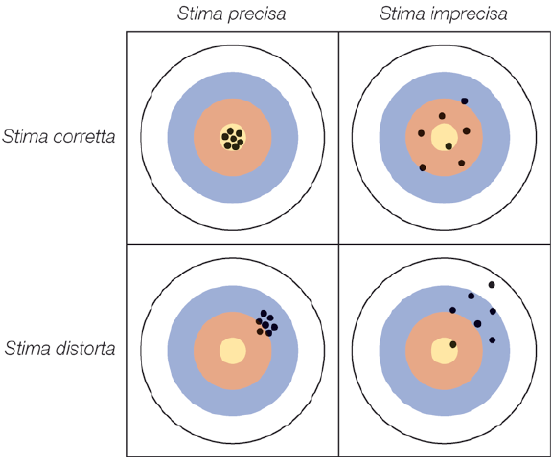
\includegraphics[width=0.6\textwidth]{fig1.2-2}
    \caption{\small{}}
    \end{figure}
La \textbf{variabilità} della misura di una caratteristica può avere molte fonti:
\begin{itemize} \tightlist
    \item \textbf{naturale}, insita nelle caratteristiche che vogliamo misurare; 
    \item \textbf{strumentale}, dovuta all'imprecisione degli strumenti; 
    \item \textbf{metodologica}, insita nell'uso improprio degli strumenti o nell'uso degli strumenti non adeguati; 
    \item \textbf{dell'operatore}, dovuta all'abilità dell'operatore, che è soggettiva e dipende da esperienza personale e molti altri fattori (stanchezza, stato emotivo, aspettative, autorità, ecc.); data la possibilità di questo tipo di variabilità è utile documentare minuziosamente la misurazione;
    \item \textbf{campionaria}, dipende dal campione selezionato, che solitamente non rispecchia perfettamente la popolazione statistica ed è comunque generalmente differente dal campione che si sceglierebbe randomicamente in un'alta situazione; ciò genera una variabilità ulteriore, oltre a quella propria della popolazione statistica. Maggiori sono le dimensioni del campione, minore è la variabilità campionaria.
\end{itemize}
La \textbf{convergenza della stima al parametro} dipende dalla grandezza dell'N campionario.

\section{Dati e variabili}
Una volta ottenuto un campione, si può cominciare a misurare le variabili di interesse.
\\
Una variabile è una qualsiasi caratteristica quantitativa o qualitativa delle unità statistiche, che si presenta in esse con un certo valore (es. sesso, peso, colore dei capelli, velocità di corsa) e che ha una variabilità intrinseca. Sono variabili anche le stime (es. velocità media di corsa di un campione casuale di 10 individui), perché esse differiscono, per effetto del caso, da campione a campione.
\\
\\
Una variabile latente è una variabile che non può essere misurata direttamente, ma dev'essere estrapolata dalla misura di altre variabili caratterizzabili in maniera quantitativa o qualitativa.
\\
Le variabili possono essere qualitative, quantitative, categorie/classi.
\\
La variabile può essere una caratteristica/attributo/campo/colonna misurabile.
\\
\\
I dati sono i risultati grezzi delle misurazioni di una o più variabili effettuate su un campione di individui.
\clearpage
A partire dalle misurazioni si caratterizzano le variabili, le quali possono essere:
\begin{itemize} \tightlist
    \item \textbf{Qualitative (categoriche)}. Descrivono caratteristiche che non possono essere misurate con un numero ma che permettono di inserire gli elementi di un campione in una categoria o gruppo (es. modalità di trasmissione di malattie: acqua, aria, vettore animale, contatto diretto).
    \item \textbf{Quantitative}. Le misure degli individui sono quantitative e ad esse è associato un valore su una scala numerica (es. conteggi, dimensioni, angoli, tassi, percentuali).
\end{itemize}
Un altro modo (preferibile) per classificare i tipi di variabili è:
\begin{itemize} \tightlist
    \item \textbf{Nominale}. Sono qualitative, categoriali e le differenti categorie non hanno un ordine intrinseco, ma solo un nome (es. gruppo sanguigno). La variabile nominale risponde solo alla domanda “a che classe l'unità campionaria appartiene”, restituendo, dunque, l'identità degli elementi del campione in base alla variabile misurata.
    \item \textbf{Ordinale}. Sono quantitative nel senso che i valori corrispondenti possono essere ordinati nonostante non siano rappresentabili su una scala numerica (es. fase biologica: uovo, larva, giovane, adulto; stato di salute; colore dei capelli, a meno di non misurarlo con uno strumento quale un esposimetro che potrebbe rendere questa categoria continua). La variabile ordinale categorizza le unità campionarie (restituisce la loro identità) e le pone in un rango.
    \item \textbf{Continue}. Sono quantitative. I valori corrispondenti appartengono a categorie continue (es. temperature, peso, lunghezza). La variabile continua categorizza le unità campionare, le inserisce in un rango e definisce degli intervalli (si può conoscere la distanza tra due misurazioni). In alcuni casi (es. peso, lunghezza) si aggiunge l'informazione di rapporto, dato che sono scale assolute (una temperatura di 30°C non è il doppio di una temperatura di 15°C, a meno che le misure non si effettuino in scala Kelvin, che è una scala assoluta).
    \\
    Nel caso in cui si tratti di variabili numeriche, queste possono assumere qualsiasi valore numerico reale in un certo intervallo di variazione. Tra due valori qualsiasi di una variabile continua possono esistere infiniti altri valori (es. temperatura corporea, area di un territorio).
    \item \textbf{Numeriche discrete}. Si presentano in unità indivisibili (es. conteggi, numero di accoppiamenti durante la stagione riproduttiva, numero di aminoacidi in una proteina).
\end{itemize}
L'età è effettivamente una variabile continua, ma a seconda delle possibilità di misurazione può anche essere considerata ordinale.
\\
La misurazione di una variabile qualitativa permette di suddividere l'unità campionaria in gruppi (es. M/F).
\\
Se si passa da una variabile continua ad intervalli si perdono informazioni e la variabile diventa categoriale ordinale. Passare da variabili continue a variabili ordinali può essere utile quando non ci si fida delle misurazioni effettuate (è come concedersi un margine d'errore).
\\
Il fatto che una variabile venga indicizzata con un numero non significa che sia una variabile numerica; si potrebbero usare i numeri anche per denominare categorie. I dati numerici possono essere ridotti a dati categorici attraverso un loro raggruppamento (es. in due gruppi: sopra e sotto la media) ma, in questo modo, parte dell'informazione viene persa.
\\
Nell'analisi statistica si cerca sempre di prevedere una delle variabili, detta \textbf{variabile risposta}, in base a una seconda variabile, detta \textbf{variabile esplicativa}. Le variabili vengono talvolta classificate come variabili indipendenti o dipendenti; questi termini sono sinonimi di variabili esplicative e risposta, rispettivamente, ma, a rigore, se una di due variabili dipende dall'altra, allora nessuna delle due è indipendente.
\clearpage
\section{Distribuzioni di frequenza e distribuzioni di probabilità}\footnote{non fatto a lezione}
Gli individui in un campione hanno generalmente diversi valori della grandezza analizzata. Si può osservare questa variabilità considerando una distribuzione di frequenza. La \textbf{frequenza} di una particolare misura in un campione è il numero di osservazioni di un determinato valore della misura. La \textbf{distribuzione di frequenza} rappresenta la frequenza con cui ciascun valore della variabile si presenta nel campione.
\\
Si usa la distribuzione di frequenza di un campione per acquisire informazioni sulla distribuzione della variabile nella popolazione dalla quale il campione è stato estratto.
\\
\\
La distribuzione di una variabile in tutta la popolazione è detta \textbf{distribuzione di probabilità}.
\\
\\
Nel caso di una variabile continua (es. spessore del becco nei fringuelli delle Galapagos), la distribuzione nella popolazione viene approssimata spesso con una distribuzione di probabilità teorica, detta distribuzione normale o di Gauss.

\section{Tipi di studi}\footnote{non fatto a lezione}
In biologia, i dati si ottengono da uno studio sperimentale o da uno studio osservazionale.
\\
\\
In uno \textbf{studio sperimentale}, il ricercatore assegna casualmente differenti gruppi di trattamento o valore di una variabile esplicativa alle singole unità di studio.
\\
\\
In uno \textbf{studio osservazionale}, è la natura ad assegnare gruppi di trattamenti o valori di una variabile esplicativa agli individui, ed il ricercatore non ha alcun controllo su quali unità rientrano in quali gruppi.
\\
\\
Una differenza fondamentale fra studi sperimentali ed osservazionali sta nel fatto che, mentre i primi possono determinare le relazioni di causa ed effetto tra le variabili, i secondi sono in grado soltanto di individuare associazioni.
(non spiegato a lezione)

\chapter{Archiviazione dei dati (B1)}

Quando si organizzano i dati che si hanno a disposizione si devono considerare due aspetti: quali sono le \textbf{unità campionarie} e quali sono le \textbf{qualità} che sono state misurate (o valutate) su queste unità statistiche. Una volta chiari questi aspetti, si può compilare una \textbf{tabella di dati}, in cui, solitamente, ad ogni colonna corrisponde una variabile, ad ogni riga corrisponde un'unità statistica, e ad ogni cella un dato.
\\
È sempre necessaria la presenza di un \textbf{campo chiave} che identifichi univocamente le unità statistiche.
\\
È importante mantenere una \textbf{uniformità di formato} in ciascuna colonna (una stessa colonna deve ospitare dati che abbiano sempre uno stesso formato, es. numerico, alfabetico, alfa-numerico).
\\
Il modo migliore per identificare un \textbf{valore mancante} è lasciare il campo vuoto (non si usa lo zero, poiché quello è effettivamente un valore) o utilizzare la sintassi specifica richiesta dal programma che si sta utilizzando (es. NA, NULL, -).
\\
Una volta scelti dei \textbf{codici} per operare è importanti che questi siano \textbf{uniformi} (es. se per indicare che un individuo è maschio si usa “m” non si può utilizzare anche “M” o “male”, etc.)
\\
\\
\textbf{Excel} è uno strumento di calcolo su fogli elettronici, non un database.
\\
In un database, ogni variabile è definita precisamente e non è possibile inserire dati che non siano corrispondenti a una formattazione prefissata, mentre in un foglio di calcolo questo inserimento è possibile. Le righe, inoltre, nei database, rappresentano solo le unità statistiche, mentre la prima riga nei fogli di calcolo solitamente rappresenta le etichette.
\\
In un foglio di calcolo è utile creare un foglio di “LUT”, ossia una “\textbf{look-up table}", un foglio di calcolo in cui vengono descritte le variabili che è possibile trovare nel primo foglio. In ogni LUT (una per ciascuna variabile considerata) vanno inseriti (etichetta colonne):
\begin{itemize} \tightlist
    \item codice (i vari dati che è possibile inserire);
    \item descrizione (la descrizione di ogni possibile dato);
    \item eventuali note.
\end{itemize}
Questo non è necessario nel caso sia presente un'interfaccia grafica che restringe la possibilità di immissione nelle celle ai soli valori della look-up table che faccia scegliere da una lista precisa la codifica corretta (es. i vari form su internet in cui, ad esempio, si inserisce la propria provincia di residenza scegliendola da una lista definita e non inserendo i singoli caratteri autonomamente).
\\
La look up table non si usa per le variabili continue, al limite è possibile in alcuni casi definire degli intervalli di valori continui che è possibile inserire, ma generalmente non è necessario.
\\
Le colonne di variabili non devono essere ridondanti, ovvero non devono essere presenti due variabili che indichino una stessa caratteristica.

\chapter{Visualizzazione dei dati (B1)}\footnote{Capitolo 2, Whitlock and Schluter, Analisi statistica dei dati biologici (2010)}
\\
La visualizzazione dei dati è fondamentale per la divulgazione e la comprensione dei risultati.
\\
\\
Regole basilari:
\begin{itemize} \tightlist
    \item identificare il messaggio;
    \item essere consapevoli che ciò che si sta presentando è importante;
    \item non spaventare i destinatari con i numeri;
    \item massimizzare la risoluzione dell'immagine;
    \item evitare immagini 3D quando non necessarie (es. barre 3D in istogrammi);
    \item usare il tipo di rappresentazione idoneo;
    \item non mischiare tipi di grafico inutilmente;
    \item non usare gli assi per confondere;
    \item non fare troppo affidamento al colore e usarlo per trasmettere un significato.
\end{itemize}
Differenti tipi di grafici possono essere utilizzati per rappresentare stessi dati; la scelta deve dipendere dal tipo di obiettivo che si ha, poiché grafici differenti sottolineano aspetti differenti.

\section{Rappresentare le distribuzioni di frequenza}
La frequenza relativa è la frazione di osservazione di una data misura, calcolata com'è il rapporto tra la frequenza (assoluta) è il numero totale di osservazioni. La distribuzione di frequenza relativa mostra la proporzione di occorrenze di ciascun valore nell'insieme dei dati.
\\
Sono disponibili diversi metodi per visualizzare graficamente le distribuzioni di frequenza, a seconda che la variabile si è categorica o numerica.

\subsection{Visualizzare variabili categoriche}
Una \textbf{tabella di frequenza} è una visualizzazione testuale del numero di occorrenze di ciascuna categoria nel dataset.
\\
\\
Un \textbf{diagramma a barre} impiega l'altezza di rettangoli per visualizzare la frequenza (assoluta o relativa) di occorrenza di ciascuna categoria. Sull'asse delle ordinate può essere rappresentata la frequenza assoluta o la frequenza relativa.
\\
Quando si trattano variabili nominali, le categorie non hanno un ordine intrinseco, ma si può semplificare il confronto della loro importanza relativa disponendole in ordine di occorrenza dalla più alla meno frequente.
\\
Nei diagrammi a barre non si riescono a distinguere le frequenze esatte, ma si ha un quadro chiaro e immediato di come i valori numerici dei crescano rapidamente nelle categorie meno frequenti. 
\\
\colorbox{lyellow}{\parbox{0.98\textwidth}{Una variabile nominale si può descrivere con un grafico a barre in cui i valori della variabile nominale sono sulle ascisse mentre sulle ordinate si riporta la percentuale dei casi in cui si sono presentate le singole variabili. Le variabili possono essere elencate in ordine alfabetico o dalla meno alla più frequente, a seconda dell'obiettivo che si ha.}}
\\
Per essere efficace, un diagramma a barre dovrebbe seguire alcune regole generali:
\begin{itemize} \tightlist
    \item nel caso di una variabile categorica ordinale (es. grado di gravità del morso di un serpente), i valori lungo l'asse orizzontale dovrebbero essere ordinati in modo naturale;
    \item nel caso di variabili categoriche nominali, l'ordinamento delle categorie secondo la frequenza con cui si osservano facilita la rappresentazione visiva delle informazioni;
    \item i rettangoli dovrebbero essere di uguale larghezza e ciascuno di essi dovrebbe poggiare su una linea base di riferimento corrispondente a y = 0, affinché l'area e l'altezza di ciascuno siano direttamente proporzionali alla frequenza; una frequenza base diversa da zero o una larghezza dei rettangoli disuguale fornirebbe una visione distorta dell'importanza relativa di ciascuna categoria;
    \item i rettangoli dovrebbero essere separati, non addossati tra loro;
    \item è utile indicare il numero totale di osservazioni (n) nella didascalia della figura.
\end{itemize}
Un \textbf{grafico a torta} è una valida alternativa attraverso la quale si possono visualizzare sia la frequenza assoluta che la frequenza relativa (ossia percentuale) dei casi.

\subsection{Visualizzare variabili numeriche}
Una distribuzione di frequenza per una variabile numerica può essere visualizzata come una tabella di frequenza o con un istogramma.
\\
\\
In un \textbf{istogramma} si rappresentano i valori di una variabile che si può assumere continua; un istogramma differisce da un grafico a barre in quanto l'ascissa non contiene le singole categorie nominali, ma categorie che raggruppano le singole categorie nominali in base ad una loro caratteristica (es. invece di inserire le varie specie sull'asse delle x, si inseriscono categorie di abbondanza, in modo da rappresentare con l'istogramma la frequenza delle specie che hanno una determinata abbondanza).\\
    \begin{figure}[h]\label{fig2.1-2}
    \centering
    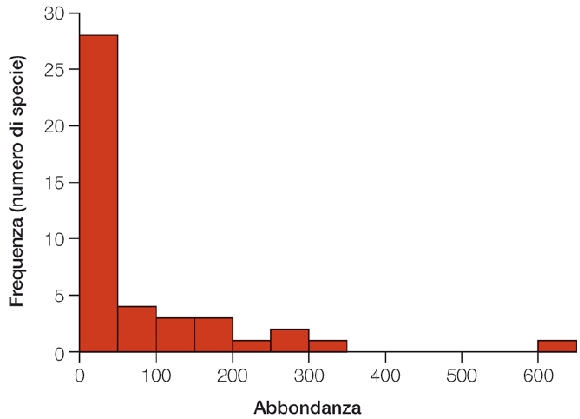
\includegraphics[width=0.6\textwidth]{fig2.1-2}
    \caption{\small{}}
    \end{figure}

La somma delle superfici di un grafico rappresentato mediante istogramma è uguale al numero totale di specie. Se invece di rappresentare la frequenza assoluta se ne rappresentasse la frequenza relativa, la somma delle aree dei rettangoli corrisponderebbe ad 1.
\\
Un istogramma utilizza l'area di bar rettangolari per visualizzare la frequenza. I valori dei dati vengono suddivisi in intervalli consecutivi (\textbf{bin}) generalmente di uguale ampiezza, e viene rappresentata la frequenza delle osservazioni che cadono in ciascun bin. 
\\
Anche se l'asse delle ordinate riporta la frequenza (assoluta o relativa) in un certo intervallo, l'istogramma deve essere inteso come rappresentazione areale: sono le aree dei vari rettangoli che devono essere proporzionali alle frequenze corrispondenti, non le altezze. Quando tutti i bin hanno la stessa ampiezza, comunque, ragionare in termini di altezze o di aree delle barre è indifferente. Se però si decidesse di raggruppare due bin in un solo intervallo, lasciando gli altri inalterati, l'altezza della nuova barra con la base più larga non dovrebbe essere pari alla somma delle frequenze nei due bin, ma alla loro media. Solo in questo modo la rappresentazione della distribuzione di frequenza basata sulle aree delle barre risulterebbe non distorta. Alternativamente si potrebbe rappresentare sull'asse delle ordinate, per ogni intervallo, non la frequenza delle osservazioni ma la densità, cioè la frequenza divisa per l'ampiezza dell'intervallo. In questo modo l'area dei rettangoli sarebbe uguale, non solo proporzionale, alla frequenza, essendo il prodotto della base (l'ampiezza dell'intervallo) per l'altezza (la densità).
\\
\\
L'istogramma di solito si usa per descrivere variabili tipicamente continue. Nel caso delle variabili nominali, l'istogramma dice solo quante sono le specie che hanno diverse classi di abbondanza (le unità statistiche non sono più i singoli uccelli osservati, ma le specie e la proprietà osservata è il numero di specie).
\\
\\
Un intervallo nella distribuzione di frequenza notevolmente più frequenti di quelli circostanti è detto \textbf{picco}.
\\
La \textbf{moda} è l'intervallo corrispondente al picco più alto.
\\
Un istogramma può assumere diverse forme, che riflettono diversi tipi di distribuzioni:
\begin{itemize} \tightlist
    \item \textbf{uniforme}: la frequenza delle varie categorie è molto simile;
    \item \textbf{a campana (normale)}: il valore centrale è quello più frequente e a partire da esso si ha un simmetrico decremento della frequenza (spesso, le biometrie presentano questa distribuzione);
    \item \textbf{a campana asimmetrica}: il decremento rispetto al picco non è uniforme nelle due direzioni (es. livello di infezione da parassiti negli animali: pochi soggetti che portano molti parassiti);
    \item \textbf{bimodale}: ci sono due modalità di distribuzione che indicano la potenziale presenza di due popolazioni statistiche.
\end{itemize}
Una distribuzione di frequenza è detta distribuzione \textbf{simmetrica} se il pattern di frequenze nella metà sinistra del istogramma è l'immagine speculare del pattern nella metà destra. La distribuzione uniforme e la distribuzione a campana sono simmetriche. Una distribuzione di frequenza che non è simmetrica è detta \textbf{asimmetrica}. Una distribuzione di frequenza per una variabile numerica, se non è simmetrica, può essere asimmetrica \textbf{positiva} (a destra) o \textbf{negativa} (a sinistra) a seconda della posizione della coda più lunga.
\\
Valori estremi molto distanti dal resto delle osservazioni sono detti \textbf{outlier} (valori anomali). Gli outlier sono comuni nei dati biologici: possono derivare da errori commessi nella registrazione dei dati o possono rappresentare caratteristiche reali della natura. Gli outlier dovrebbero essere sempre analizzati attentamente e si dovrebbe eliminarli dall'insieme dei dati soltanto se si riesce a dimostrare che sono frutto di errori.
\\
\\
L'ampiezza degli intervalli di un istogramma può influenzare le conclusioni tratte dal grafico.
\\
L'ampiezza delle classi (bin) ed il loro numero sono legati, e definirli è importante poiché si tratta di fattori che influenzano la risoluzione dei casi (es. una distribuzione bimodale potrebbe sembrare una asimmetrica se i bin venissero allargati).
\\
Per definire ampiezza e numero delle classi si può ricorrere a diversi approcci, ad esempio:
\begin{itemize} \tightlist
    \item \textbf{H. Sturgess} (1926):
    \begin{equation}
        C = 1 + \frac{10}{3}\ log_{10}(N)
    \end{equation}
    In cui C è pari al numero di classi.
    \item \textbf{D. Scott} (1979):
    \begin{equation}
        h = \frac{3.5 \cdot s}{\sqrt{N}}
    \end{equation}
    In cui h è l'ampiezza delle classi, ed s è la deviazione standard.
\end{itemize}
In entrambi i casi, N è la dimensione campionaria.
\\
Non esistono regole rigorose riguardo al numero di intervalli che si devono usare nelle tabelle di frequenza e negli istogrammi; alcuni programmi impiegano la regola empirica di Sturges, in cui il numero di intervalli è 1 + ln(n)/ln(2), in cui n è il numero di osservazioni. Il numero di intervalli che si ottiene con questa formula viene poi arrotondato al numero intero più alto. 
\\
In generale, si dovrebbe scegliere il numero di intervalli in modo da far risaltare nella maniera migliore i pattern e le eccezioni nei dati, il che richiede buon senso piuttosto che regole rigorose.
\\
\\
Per costruire un istogramma si dovrebbero seguire alcune semplici regole:
\begin{itemize} \tightlist
    \item il lato inferiore di ogni rettangolo deve giacere sulla linea di base corrispondente a y = 0, affinché le aree siano proporzionali alle frequenze;
    \item diversamente da quanto accade nei diagrammi a barre, i rettangoli vicini di un istogramma non sono separati, il che rafforza la percezione di una scala numerica, grazie al passaggio graduale da ciascun rettangolo a quello successivo;
    \item quando si suddividono i dati in intervalli si devono usare numeri facilmente leggibili per i punti di suddivisione tra intervalli (es. 0.5 invece che 0.482);
    \item è utile indicare il numero totale di individui nella didascalia che accompagna l'istogramma.
\end{itemize}

\section{Quantili di una distribuzione di frequenza}
Tutte le informazioni relative alla forma della distribuzione di frequenza di una variabile numerica sono contenute nei suoi percentili e nei quantili strettamente correlati. 
\\
\\
L'x-esimo \textbf{percentile} di una distribuzione è il valore al di sotto del quale è situato l'x\% degli individui; lo stesso valore anche rappresentabile attraverso il \textbf{quantile} x/100.

\section{Distribuzione di frequenza cumulativa}
La \textbf{distribuzione di frequenza cumulativa} è il diagramma di tutti i quantili di una variabile numerica. Per costruire una distribuzione di frequenza cumulativa dell'abbondanza di tutte le specie di uccelli del deserto dell'Esempio 2.1B, prima sono state ordinate tutte le misure dalla più piccola alla più grande, poi è stata calcolata la frazione di os- servazioni minori o uguali a ciascun valore. Questa frazione, detta frequenza relativa cumulativa, è rappresentata graficamente dall'altezza della curva sopra il corrispondente valore osservato nei dati. Ogni gradino è piatto, ma la curva si innalza di 1/n in corrispondenza di ogni misura osservata, dove n è il numero di osservazioni, fino a un massimo di 1. Possono esservi salti più grandi di 1/n in corrispondenza di una misura se la stessa misura si ripete in più punti. La curva fornisce molti particolari perché illustra ogni singola osservazione.
\clearpage
    \begin{figure}[h]\label{fig2.2-1}
    \centering
    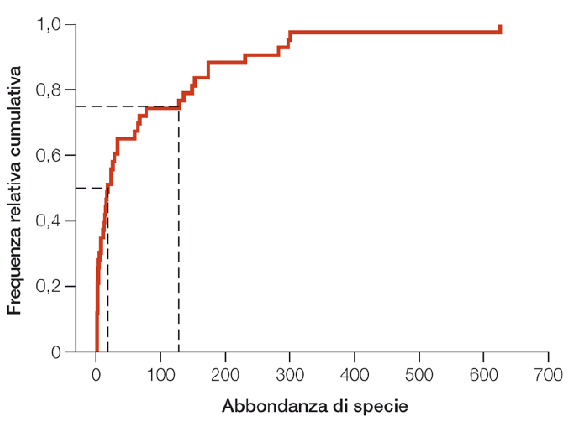
\includegraphics[width=0.6\textwidth]{fig2.2-1}
    \caption{\small{}}
    \end{figure}

\section{Associazioni tra variabili categoriche}
La visualizzazione dei dati è molto utile quando si studiano l'associazione tra variabili e le differenze tra gruppi. I metodi che si usano per presentare graficamente le relazioni dipendono dai tipi di variabili di interesse, cioè dal fatto che esse siano categoriche oppure numeriche.
\\
\\
Le \textbf{tabelle di contingenza} sono tabelle di frequenza per due o più variabili categoriche che mostrano come i valori di una variabile siano associati e valori di una seconda variabile. 
\\
Una cella è una combinazione di categorie delle variabili riga e colonna. La variabile esplicativa è presentata nelle colonne, mentre la variabile risposta, quella che viene prevista, è presentata nelle righe. 
\\
\\
Il \textbf{diagramma a barre raggruppate} si rettangoli per rappresentare graficamente la frequenza di tutte le combinazioni di due (o più) variabili categoriche.
\\
I diagrammi a barre raggruppate seguono tutte le convenzioni valide per i diagrammi a barre, con la differenza che i gruppi (per esempio, malaria e assenza di malaria) sono indicati con differenti colori o sfumature di colore.  Lo spazio tra i rettangoli dei diversi gruppi della variabile esplicativa (per esempio, controllo e sottrazione di uova) è bene che sia più ampio dello spazio tra i rettangoli della variabile risposta.
\\
\\
Un \textbf{grafico a mosaico} (mosaic plot, diagramma di Marimekko) è simile a un diagramma a barre raggruppate, con la differenza che i rettangoli relativi allo stesso gruppo sono impilati l'uno sull'altro invece di essere disposti fianco a fianco.
\\
L'area dei rettangoli in un grafico a mosaico rappresenta la frequenza relativa (ossia la proporzione) entro ciascun gruppo.
\\
La larghezza di ciascuna di la verticale è direttamente proporzionale al numero di osservazioni per quel gruppo.
\\
L'area di ciascun rettangolo, quindi, è direttamente proporzionale alla frequenza relativa di quella combinazione di variabili nell'intero insieme di dati.
\\
L'ordine dei gruppi lungo l'asse orizzontale è predeterminato nel caso dei dati ordinali ed arbitrario nel caso dei dati nominali.
\\
Un grafico a mosaico fornisce una panoramica dei dati e consente di riconoscere le relazioni tra variabili considerate. Ad esempio, l'indipendenza viene mostrata quando le caselle nelle categorie hanno tutte le stesse aree. L'area delle tessere, nota anche come dimensione del bin, è proporzionale al numero di osservazioni all'interno di quella categoria.
\\
\begin{figure}[h]\label{fig2.3-2}
    \centering
    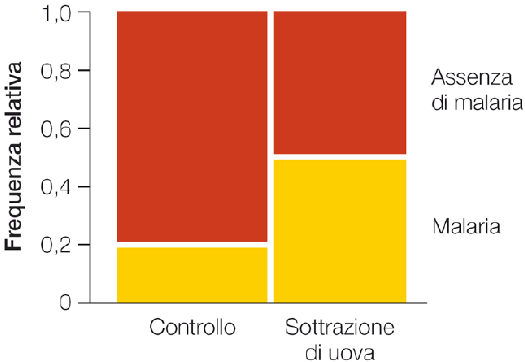
\includegraphics[width=0.5\textwidth]{fig2.3-2}
    \caption{\small{}}
    \end{figure}
\\
Il principale vantaggio del diagramma a barre raggruppate, rispetto alla tabella di contingenza, è il fatto che risulta più facile confrontare visivamente l'altezza o l'area dei rettangoli che i numeri.  Questo vantaggio si riduce se le variabili esplicative e le variabili hanno molte categorie, poiché in questo caso aumenta la complessità del diagramma. Il grafico a mosaico, d'altra parte, è più semplice da leggere rispetto al diagramma a barre raggruppate.
\\
Per decidere quale tipo di visualizzazione sia più efficace per una data circostanza è meglio sperimentare più metodi e scegliere tra essi sulla base delle informazioni che esprimono, della chiarezza e della semplicità.

\section{Confrontare variabili numeriche tra gruppi}
Gli istogrammi di frequenza relativa prescindono dalle dimensioni del campione, quindi ci si concentra su posizione e forma dell'istogramma, e non sull'altezza assoluta.
\\
\\
Dunque, un metodo utile per confrontare più distribuzione di frequenza consiste semplicemente nel costruire un istogramma per ciascun gruppo. Se poi gli istogrammi vengono presentati in serie, uno sotto l'altro, facendo attenzione che la scala dell'asse delle x sia la stessa, il confronto risulta più semplice e immediato.
\\
\\
Esempio di applicazione degli istogrammi (Fig.\ref{fig2.4-1}): livelli di emoglobina in maschi umani a diverse altitudini.\\
Sono tutte distribuzioni discretamente simmetriche. L'ipotesi (aumento della concentrazione di emoglobina nel sangue all'aumentare dell'altitudine) non sembra essere verificata, poiché i valori di tendenza centrale dei primi tre grafici sono molto simili; solo sulle Ande si riscontra una palese differenza.
\\
Prendendo tutti i dati assieme si potrebbe ottenere una distribuzione bimodale.
\\
Lo stesso confronto si può fare usando delle curve di frequenze cumulate.
\\
\\
Si può esaminare anche l'associazione tra una variabile numerica e una variabile categorica confrontando le distribuzioni di frequenze cumulative. Questo approccio presenta le distribuzioni per più gruppi in una singola visualizzazione compatta.
\clearpage
\begin{figure}[h]
    \centering
    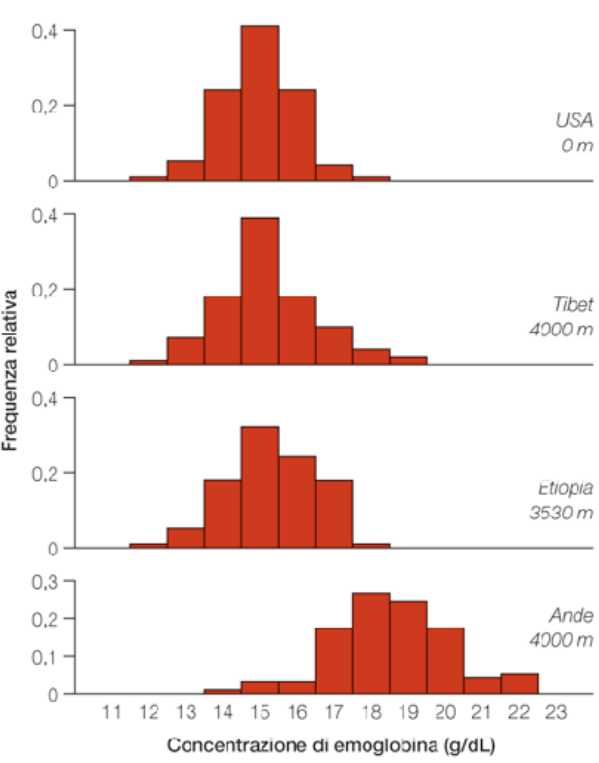
\includegraphics[width=0.6\textwidth]{fig2.4-1}
    \caption{\small{}}
    \label{fig2.4-1}
\end{figure}
\begin{figure}[h!]
    \centering
    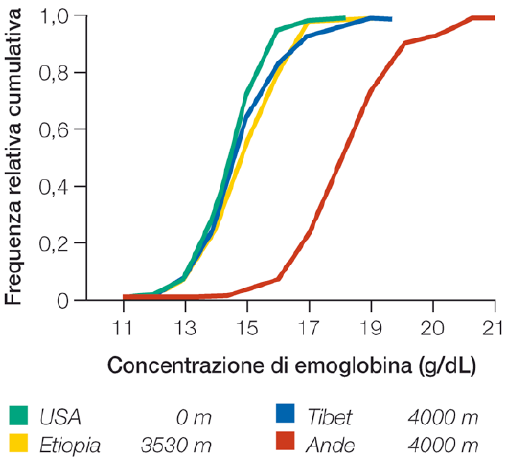
\includegraphics[width=0.5\textwidth]{fig2.4-2}
    \caption{\small{}}
    \label{fig2.4-2}
\end{figure}

\section{Visualizzare la relazione tra una coppia di variabili numeriche}
Ci sono tre metodi per visualizzare la relazione tra due variabili numeriche: diagrammi di dispersione (scatter plot), diagrammi a linee, mappe.
\\
\\
Uno \textbf{scatter plot} (diagramma di dispersione, grafico a punti) visualizza il pattern di associazione tra due variabili numeriche. Ogni osservazione è rappresentata da un punto su un diagramma formato da due assi (diagramma cartesiano). La posizione lungo l'asse orizzontale (l'asse delle ascisse o delle x) indica la misura della variabile esplicativa; la posizione lungo l'asse verticale (l'asse delle ordinate o delle y) indica la misura della variabile risposta. Il pattern, nella risultante nube di punti, indica se un'associazione tra le due variabili sia positiva (nel qual caso i punti tendono a distribuirsi nel diagramma dal basso a sinistra verso l'alto a destra), negativa (i punti tendono a decorrere dall'alto a sinistra verso il basso a destra) o assente (non c'è un pattern distinguibile). Un diagramma di dispersione riesce anche a rivelare se la relazione tra due variabili possa essere rappresentata da una retta oppure da una curva più articolata.
\\
Es. in una specie di pesci, la proporzionalità diretta tra ornamentazione del padre con l'attrattività del figlio, le unità statistiche sono le coppie padre-figlio. L'ornamentazione del padre è un proxy per l'attrattività del figlio.\\
    \begin{figure}[h]\label{fig2.5-1}
    \centering
    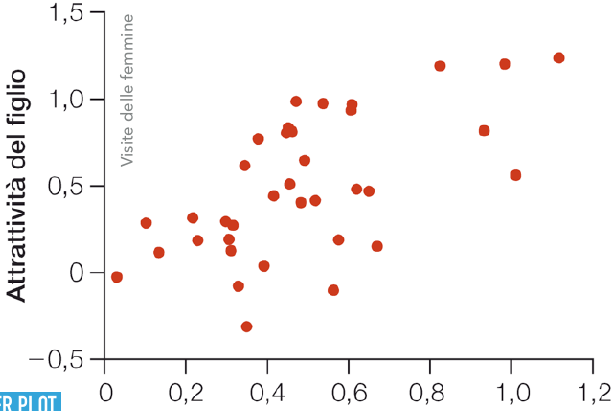
\includegraphics[width=0.6\textwidth]{fig2.5-1}
    \caption{\small{}}
    \end{figure}

Quando si ha una sequenza temporale dei dati che si stanno rappresentando si possono collegare i vari punti con una linea, ottenendo un diagramma a linee.
\\
Un \textbf{diagramma a linee} è uno strumento efficace per visualizzare tendenze nel tempo o rispetto a qualche altra variabile ordinata. Un diagramma a linee è simile a un diagramma di dispersione, eccetto che viene riportato soltanto una misura y per ogni osservazione x. I punti adiacenti lungo l'asse x sono uniti da un segmento.
\\
I segmenti di retta che congiungono i punti rendono più visibili le tendenze della popolazione. 
\\
L'inclinazione più o meno ripida dei segmenti rispecchia la velocità di variazione della popolazione.
\\
Si tratta di una serie temporale.
\clearpage
    \begin{figure}[h]\label{fig2.5-2}
    \centering
    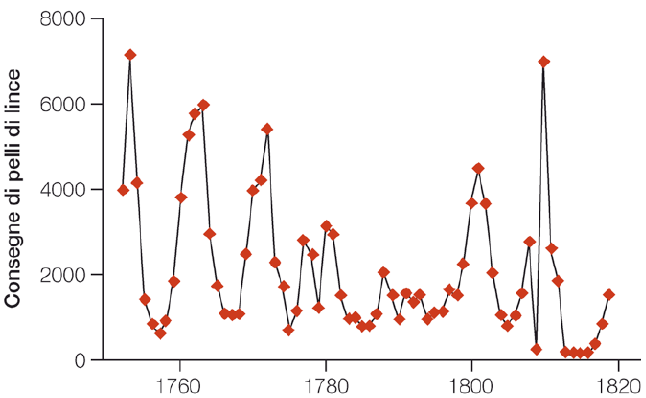
\includegraphics[width=0.6\textwidth]{fig2.5-2}
    \caption{\small{}}
    \end{figure}

Questi grafici possono mettere in evidenza meccanismi naturali (es. relazione preda-predatore: effetto rimozione, effetto disponibilità risorse per preda, effetto stress da predazione, etc).
\\
\\
Una \textbf{mappa} è l'equivalente spaziale del diagramma a linee: visualizza una misura numerica di risposta in più posizioni su una superficie. La variabile esplicativa è sempre una serie ordinata, costituita da punti nello spazio. Si visualizza una misura y per ogni punto o regione sulla superficie.
\\
Le mappe possono indicare misure in punti su qualsiasi superficie. La superficie può essere un reticolo spaziale o una regione della superficie terrestre delimitata da confini politici o geologici. Le mappe possono essere usate anche per indicare misure su rappresentazioni di qualsiasi oggetto bidimensionale o tridimensionale.
\\
\\
Le rappresentazioni grafiche e le tabelle hanno un duplice scopo: essere uno strumento per l'analisi dei dati e comunicare e sintetizzare i pattern nei dati a un pubblico più vasto. Questi obiettivi sono ampiamente convergenti, perché le visualizzazioni più informative sono anche quelle più adatte per identificare pattern nei dati e per comunicarli. In tutti i casi, la visualizzazione dei dati deve essere chiara, onesta ed efficiente.
\\
\\
Alcuni consigli generali per aumentare l'efficacia delle rappresentazioni grafiche sono:
\begin{itemize} \tightlist
    \item Mostrare i dati.
    \item Rappresentare accuratamente le grandezze. Una linea base corrispondente allo zero è essenziale nei diagrammi a barre e negli istogrammi, perché l'occhio interpreta istintivamente l'area dei rettangoli come direttamente proporzionale al valore relativo. Altri diagrammi, come il diagramma a linee, non sempre hanno questo scopo e quindi non sono vincolati a possedere questa caratteristica. L'obiettivo principale di un diagramma di dispersione è visualizzare un'associazione, non un valore numerico o una frequenza, e la scelta della linea base dovrebbe essere fatta tenendo presente questo criterio.
    \item Cose superflue sono gli effetti tridimensionali, che non soltanto non sono necessari, ma distorcono anche l'altezza e l'area dei rettangoli, ingannando di nuovo l'occhio. Questi abbellimenti inutili e ingannevoli sono noti come "chartjunk" ("spazzatura del diagramma"). Gli elementi grafici inessenziali dovrebbero essere eliminati per permettere che i pattern nei dati possano emergere con maggior chiarezza.
    \item Utilizzare elementi grafici in maniera chiara riducendo la confusione e le ridondanze.
    \item Readere la rappresentazione grafica di facile interpretazione, attraverso una scelta mirata dei caratteri tipografici e dei colori e attraverso l'indicazione delle unità di misura e l'uso di simboli grafici chiaramente distinguibili per rappresentare differenti gruppi.
    \item Identificare chiaramente gli assi.
    \item Inserire didascalie che siano self-explanatory (non deve essere necessario leggere il testo, ad esempio, dell'articolo che contiene il grafico, per interpretarlo) e dunque ridondanti rispetto alle didascalie di altri grafici presenti nello stesso lavoro o al lavoro stesso.
\end{itemize}

Le tabelle possono avere scopi diversi:
\begin{itemize} \tightlist
    \item immagazzinamento dei dati, ovvero la conservazione dei dati grezzi a scopo di riferimento; tabelle di questo tipo sono spesso grandi e non adatte alla comunicazione dei risultati finali; quando vengono pubblicate, vengono presentate di solito come appendici o allegati.
    \item visualizzazione di pattern ed eccezioni nei dati (es. tabelle di frequenza). Per produrre tabelle chiare, onesto e deficienti si devono seguire in generale gli stessi criteri già elencati per le rappresentazioni grafiche. Queste tabelle devono essere compatte e presentare il numero minimo di cifre significative necessarie ad evidenziare il pattern. L'organizzazione dei dati in tabella deve facilitare la lettura e l'identificazione delle caratteristiche principali dei dati.
\end{itemize}
I diagrammi sono il mezzo migliore per mostrare pattern ed eccezioni, ma forniscono pochi particolari quantitativi; le tabelle, quindi, sono più appropriate quando è importante comunicare anche aspetti quantitativi dei dati.
\\
\\
CONSIDERAZIONE PERSONALE
\\
La rappresentatività di un campione non dipende solo dal numero di elementi costituenti il campione, ma anche dalla variabilità del parametro al quale si è interessati (caso estremo: 0 variabilità, anche solo un elemento è rappresentativo; variabilità=2, anche quattro su 100 è più probabile che sia rappresentativo che nel caso in cui ci fosse varietà=10).
\\
(ma in effetti vale solo se si è interessati ad avere un'idea della variabilità del parametro e non del rapporto tra le n varietà del parametro).

\chapter{Statistiche descrittive (B2)}\footnote{Capitolo 3, Whitlock and Schluter, Analisi statistica dei dati biologici (2010)}
\\
I dati si possono descrivere graficamente o attraverso indici (statistiche) sintetiche.
\\
\\
I parametri delle popolazioni si indicano con lettere greche, mentre per le stime si usa il normale alfabeto.
\\
\\
Utile prima rappresentare i dati graficamente e poi in base ai risultati scegliere le statistiche descrittive adatte.
\\
\\
Una distribuzione può essere:
\begin{itemize} \tightlist
    \item \textbf{uniforme}: tutto il range di variazione della x è rappresentato in maniera uniforme nella popolazione;
    \item \textbf{a campana}: i valori centrali del range di distribuzione della x sono I più frequenti nella popolazione (molte biometrie hanno tale distribuzione);
    \item \textbf{asimmetrica}: valori di x più frequenti lontani dai valori centrali;
    \item \textbf{bimodale}: i valori di x più frequenti corrispondono a due diversi punti del range di distribuzione di x; porta a concludere che nella popolazione ci sono in realtà due popolazioni statistiche.
\end{itemize}
Per descrivere numericamente una distribuzione si deve tener conto di due sue caratteristiche:
\begin{itemize} \tightlist
    \item \textbf{tendenza centrale}: la misura che meglio descrive la maggior parte dei dati o che comunque esprime una loro centralità. Indici della tendenza centrale sono: quartili (misure di posizione) e media.
    \item \textbf{dispersione}: indica come le misure si collocano attorno a quella di tendenza centrale, rappresenta la variabilità della popolazione statistica in relazione alla variabile misurata. Misure di dispersione sono: distanza interquartile (misura di posizione), scarto medio assoluto, varianza, deviazione standard.
\end{itemize}
Le misure di posizione misurano la posizione dei valori, non le differenze tra essi in termini numerici.

\section{Misure di tendenza centrale}
Su una serie di dati ordinati in ordine crescente, i \textbf{quartili} sono i tre valori che dividono la distribuzione in quattro blocchi, ognuno dei quali rappresenta un quarto complessivo dei record (25\%). Il valore centrale è la \textbf{mediana} (o secondo quartile, il valore centrale che divide la sequenza di dati ordinati in due gruppi di eguale numerosità, 50\%), gli altri due sono il primo (il 25-esimo percentile) ed il terzo quartile (il 75-esimo percentile).
Per calcolare la mediana:
\begin{itemize} \tightlist
    \item se il numero di osservazioni \textbf{($n$) è dispari}, allora la mediana è l'osservazione centrale:
    \begin{equation}
        mediana = Y_{\frac{n+1}{2}}
    \end{equation}
    \item se il numero di osservazioni \textbf{($n$) è pari}, allora la mediana è la media della coppia centrale di valori:
    \begin{equation}
        mediana = \frac{Y_{\frac{n}{2}} + Y_{\frac{n}{2}+1}}{2}
    \end{equation}
\end{itemize}
Primo e terzo quartile non sono necessariamente simmetrici rispetto alla mediana, non si può sapere, solo conoscendo i loro valori, quanto essi siano distanti dalla mediana.
\\
\\
In generale, si parla di \textbf{quantili}, statistiche descrittive che indicano la posizione del valore nella distribuzione.
\\
I \textbf{decili} dividono la serie ordinata di numeri in blocchi di 10\%.
I \textbf{percentili} possono corrispondere ad una percentuale arbitraria.
\\
\\
I \textbf{boxplot} (box \& whiskers) sono grafici che rappresentano la variabilità dei valori rispetto ai quartili.
\\
I punti che giacciono al di fuori della distribuzione sono gli \textbf{outliers}. Si usa come criterio l'ampiezza del box: un outlier è considerato tale quando dista dal box (solitamente) più di una volta e mezzo l'ampiezza del box (si possono scegliere anche altre distanze, più o meno permissive, in base ad un ragionamento sensato).
\\
I \textbf{baffi} sono i valori estremi misurati (tra inizio distribuzione e primo quartile e tra terzo quartile ed ultimo valore), di solito il minimo ed il massimo, una volta esclusi gli outliers.
\\
Il boxplot è, dunque, una rappresentazione grafica che NON assume la simmetria della distribuzione.\\
    \begin{figure}[h]\label{fig3.2-2}
    \centering
    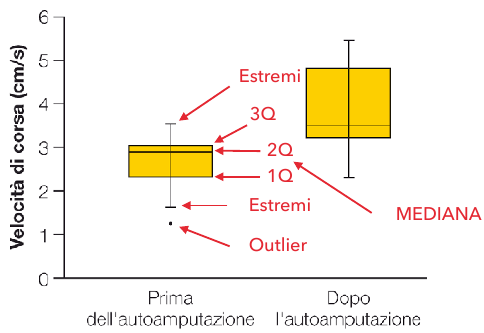
\includegraphics[width=0.6\textwidth]{fig3.2-2}
    \caption{\small{}}
    \end{figure}

La \textbf{media} è la somma di tutti i valori osservati diviso il loro numero.
\\
La \textbf{media ponderata} tiene conto del “peso” di ciascun valore, si ha quando la variabile continua è riclassificata in una variabile ordinale.
\\
Si attribuisce a ciascuna classe un valore, spesso il valore medio dell'intervallo, che si moltiplica per il numero di soggetti che hanno tale valore medio. La media ponderata è meno precisa di quella aritmetica classica.
\\
La media non discrimina tra distribuzioni con la stessa tendenza centrale ma diversa dispersione.

\section{Misure di dispersione}
La \textbf{distanza interquartile} è la misura di variabilità quando si usano statistiche descrittive basate sui quartili.
\\
\\
Per calcolare la dispersione:
\begin{itemize} \tightlist
    \item \textbf{scarto medio assoluto (Sm)}: media di quanto ciascun caso dista dal valore medio. Data la simmetria attorno alla media, i valori positivi e quelli negativi si annullerebbero, per questo è necessario considerare i valori assoluti, per cui si deve calcolare il quadrato e poi fare la radice.
    \begin{equation}
        S_m = \frac{\sum{\abs{x_i - \overline{x}}}}{n}
    \end{equation}
    \item \textbf{devianza (SQ)}: si sommano le differenze ottenute da ciascun valore, elevate alla seconda per evitare che si ottenga un valore nullo; la devianza non è pesata sul numero di casi, cosa necessaria quando si vogliono confrontare le dispersioni di popolazioni con diverso N.
    \begin{equation}
        SQ = \sum{(x_i - \overline{x})^2}
    \end{equation}
    \item \textbf{varianza (QM)}: permette di pesare la devianza sul numero di casi considerati. Si usa spesso n-1 al denominatore perché si fa una correzione: più la numerosità è elevata più la varianza campionaria è affidabile e la correzione non ha peso; quando l'N campionario è molto basso, invece, la correzione permette di non rischiare di avere una sottostima della variabilità. Tale correzione ha senso quando si fanno stime della varianza, non quando questa viene calcolata esattamente (ovvero quando si hanno i dati riguardanti tutta la popolazione statistica).
    \begin{equation}
        s^2 = \frac{\sum{(x_i - \overline{x})^2}}{n-1}
    \end{equation}
    \item \textbf{deviazione standard (o scarto quadratico medio, DS o SD)}: misura più utilizzata nelle statistiche descrittive.
    \begin{equation}
        s = \sqrt{\frac{\sum\limits_1^n{(x_i - \overline{x})^2}}{n-1}}
    \end{equation}
\end{itemize}

\section{Coefficiente di variazione}
Più la dimensione campionaria è bassa, più la variabilità misurata è elevata, quindi a volte non è immediato confrontare variabilità di distribuzioni diverse (di stessa natura o di natura diversa); esistono delle statistiche di varibailità che consentono di misurare la variabilità rispetto al valore della media; una di queste è il \textbf{coefficiente di variazione}:
\begin{equation}
    CV = \frac{\sigma}{\mu}\ 100
\end{equation}
In cui $\sigma$ è la deviazione standard, $\mu$ è la media, ed il loro rapporto viene moltiplicato per 100 perché è comodo usare le percentuali.

\section{Range ed intervallo}
Altre misure di dispersione sono i range e l'intervallo.
\\
Il \textbf{range} è la differenza tra il valore massimo ed il minimo della serie di dati, mentre l'\textbf{intervallo} definisce quali sono il valore massimo e quello minimo.

\section{Confronto tra misure di posizione e dispersione}
Queste misure alternative di posizione e di dispersione danno informazioni simili quando la frequenza di distribuzione è simmetrica e unimodale, ma la media e la deviazione standard diventano meno informative rispetto alla mediana e alla differenza interquartile quando i dati includono osservazioni estreme.
\\
\\
Alcune condizioni che si verificano quando la distribuzione è normale:
\begin{itemize} \tightlist
    \item somma degli scarti è pari a zero (quindi la media è un punto di equilibrio, mentre la mediana solo di centralità);
    \item devianza è un minimo (la distanza di tutti i punti da qualunque altro valore che non sia la media è maggiore della devianza);
    \item media delle medie ponderate è pari alla media (associatività).
\end{itemize}

\section{Mode lasche}
La \textbf{moda} è il valore più frequente della distribuzione.
\\
\\
Moda e mediana vengono dette “\textbf{mode lasche}”, perché danno relativamente poche informazioni.
\\
\\
Nelle distribuzioni normali, media, moda e mediana corrispondono.

\section{Distribuzione campionaria}
La \textbf{stima} è il processo con cui si inferisce un parametro della popolazione a partire dai dati ottenuti da un campione. ``Stima'' è anche il risultato del processo di stima.
\\
La stima non è quasi mai esattamente uguale al valore del parametro della popolazione che viene valutato, perché il campionamento è influenzato dal caso.
\\
Per conoscere la precisione della stima si deve conoscere a grandi linee come il processo di campionamento potrebbe influenzare la stima che otteniamo. Si usa a questo scopo la distribuzione campionaria della stima, cioè la distribuzione di probabilità di tutti i valori di una stima che si potrebbero ottenere campionando molte volte la popolazione.
\\
\\
La distribuzione campionaria rappresenta la "popolazione" di valori per una stima. 
\\
Non si tratta di una popolazione reale, ma una popolazione immaginaria di valori per una stima.
\\
\\
La dispersione della distribuzione campionaria di una stima dipende dalla dimensione del campione. 
\\
Più grande è la dimensione del campione, più stretta è la distribuzione campionaria. 
\\
E, più stretta è la distribuzione campionaria, più precisa sarà la stima, visto che una singola stima sarà mediamente più vicina al valore vero.
\\
\\
La distribuzione della media campionaria è normale anche se la distribuzione iniziale no.

\section{Errore standard \label{errst}}
La distribuzione campionaria si usa per misurare la precisione di una stima.
\\
La deviazione standard della distribuzione campionaria di una stima è detta \textbf{errore standard (ES)}. Dato che riflette le differenze tra una stima e il parametro preso in considerazione, l'errore standard misura la precisione della stima. Le stime affette da errori standard più piccoli sono più precise di quelle affette da errori standard più grandi: minore è l'errore standard, minore è l'incertezza riguardo al parametro della popolazione. 
\begin{equation}
    ES = \frac{s}{\sqrt{n}}
\end{equation}
In cui $s$ è la deviazione standard della stima.
\\
Quando si usa la deviazione standard, dato che questa si basa sulla media, si sta assumendo che la distribuzione almeno tenda alla normalità.
\\
\\
Tutte le statistiche parametriche si basano sulla media; nel momento in cui la media non è un buon descrittore, non si possono usare più statistiche parametriche.
\\
\\
Quando si riporta una media, si deve almeno indicare l'errore standard.

\chapter{Distribuzione normale (B2)} \footnote{Capitolo 10, Whitlock and Schluter, Analisi statistica dei dati biologici (2010)}
\\
Con $n$ molto alti ci si può permettere di avere bin di ampiezza molto ridotta che, una volta rappresentati, possono essere approssimati da una curva.
\\
\\
La misura di tendenza centrale più informativa nei casi di distribuzione normale è la media aritmetica, che in tali casi corrisponde con moda e mediana.
\\
\\
La distribuzione normale è molto comune in natura (molte biometrie seguono una distribuzione normale), probabilmente perché i processi che si osservano in natura sono il risultato di un processo di selezione.
\\
\\
I parametri che determinano la forma delle curve normali sono media e varianza ($\sigma^2$), mentre gli altri sono costanti.
\\
\\
Le curve \textbf{platicurtiche} sono schiacciate (es. viola), mentre le  \textbf{leptocurtiche} sono appuntite (es. rossa).\\
\begin{figure}[h]\label{normalcurvetypes}
    \centering
    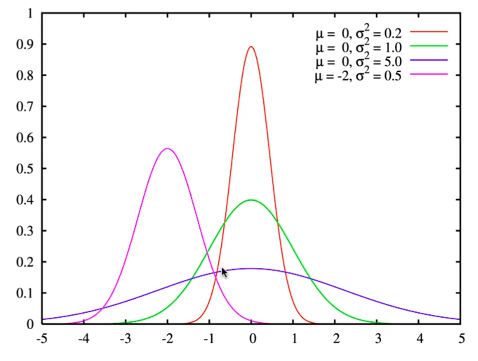
\includegraphics[width=0.6\textwidth]{normalcurvetypes}
    \caption{\small{}}
\end{figure}

Le curve normali sono asintotiche rispetto all'asse delle x.
\\
\\
La \textbf{curva normale standardizzata}, che ha media 0 e varianza 1, si può ottenere a partire da una distribuzione normale qualsiasi di una qualsiasi variabile continua. Considerando una curva normale, si trasforma ogni valore della distribuzione ($y_i$) in unità di deviazione standard ($Z$):
\begin{equation}
    Z = \frac{y_i - \overline{y}}{s}
\end{equation}
In cui $s$ è la deviazione standard osservata per il campione.
\\
Il valore ottenuto fa capire se il valore corrispondente sta sopra o sotto la media rispetto ad una misura di variabilità.\\
\begin{figure}[h]\label{standardizednormalcurve}
    \centering
    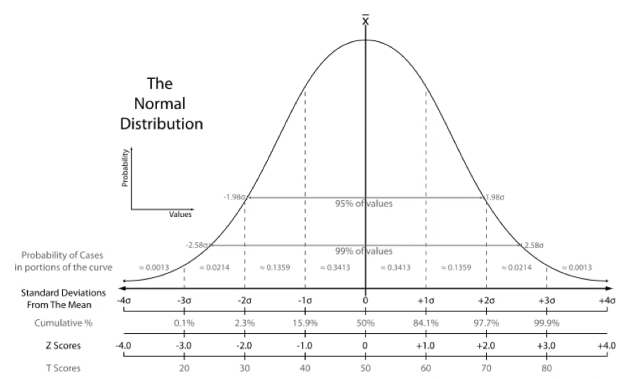
\includegraphics[width=\textwidth]{standardizednormalcurve}
    \caption{\small{no 1.98 ma 1.96 volte $\sigma$.}}
\end{figure}

Con riferimento alla distribuzione standardizzata, il 95\% dei valori ricade all'interno dell'intervallo che si estende tra -1.96 volte la deviazione standard e +1.96 volte la deviazione standard, mentre tra -1 e +1 volta la deviazione standard si ha il 66.27\% dei casi.
\\
La curva normale standardizzata ha proprietà definite.
\\
\\
In un boxplot di una distribuzione normale, il 50\% dei casi è racchiuso nel box.
\\
\\
Queste considerazioni valgono anche per la distribuzione campionaria delle medie.
\clearpage
\begin{figure}[h]\label{standardizednormalcurve2}
    \centering
    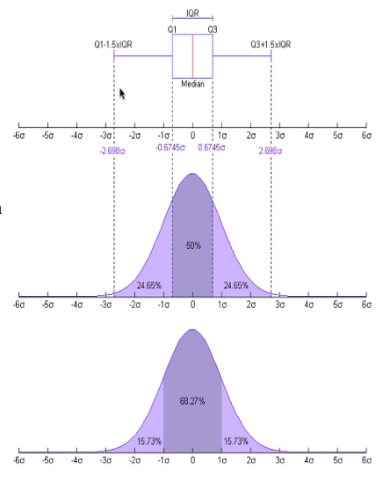
\includegraphics[width=0.75\textwidth]{standardizednormalcurve2}
    \caption{\small{}}
\end{figure}

\section{Teorema del limite centrale}
La sommatoria di molte distribuzioni distribuite in meniera non normale genera una distribuzione normale.
\\
\\
Secondo il \textbf{teorema del limite centrale}, la somma o la media di n misure da una distribuzione quasi o non normale genera una distribuzione normale.

\section{Intervallo di confidenza}
L'errore standard è la misura della ds nella media campionaria. Siccome, per la media campionaria, l'errore standard è uguale alla ds per una variabile qualsiasi, anche in questo modo si può indicare la precisione della media.
\\
\\
Per la curva normale, se si campiona n volte, nel 95\% dei casi, la media avrà un intervallo di confidenza che ricadrà tra $media-1.96*ES$ e $media+1.96*ES$.
\\
\\
In questo modo gli IC possono essere usati come metodo inferenziale.

\chapter{Probabilità (B3)}\footnote{Capitolo 5, Whitlock and Schluter, Analisi statistica dei dati biologici (2010)}
\\
Lo \textbf{spazio campionario} è la lista di tutti i possibili risultati di una prova casuale.
\\
Una \textbf{prova} è \textbf{casuale} quando è aleatoria.
\\
Un \textbf{evento} è un qualsiasi sottoinsieme potenziale dello spazio campionario. Per esempio, se lanciamo un dado a 6 facce, sono possibili 6 risultati: i numeri da 1 a 6. Questi 6 differenti numeri rappresentano nel loro insieme lo spazio campionario. Possiamo definire molti eventi che potrebbero interessare, quali "il risultato è un numero pari", "il risultato è un numero maggiore di 3" o anche il semplice evento "il risultato è 4". 
\\
La \textbf{probabilità} di un evento è la proporzione di tutte le prove casuali in cui si verifica l'evento specificato rispetto a tutti gli eventi possibili, quando la stessa prova casuale viene ripetuta un tot di volte in \underline{condizioni definite}.
\\
La proporzione di casi di uno degli eventi dello spazio campionario sul totale degli eventi possibili è la migliore \underline{stima} della probabilità di tale evento.
\\
Le probabilità, essendo proporzioni, devono essere sempre comprese tra 0 e 1, estremi inclusi: un evento ha probabilità 0 se non si verifica mai e ha probabilità 1 se si verifica sempre.
\\
La sommatoria di tutte le probabilità di tutti gli eventi possibili è pari a 1.
\\
\\
Es. lanciando un dado, ogni lancio (prova casuale) può risultare in una qualsiasi delle sei facce del dado (spazio campionario), e c'è una probabilità di $\frac{1}{6}$ che una determinata faccia esca.
\\
\\
Un evento può essere anche una combinazione di più eventi (es. lanciando il dado due volte, probabilità che esca un 2 ed un 5?), ed è definito da una probabilità (quante volte si osserva un dato evento sul totale delle volte che si compie l'osservazione).

\section{Istogrammi di frequenza}
Si potrebbe creare un istogramma di frequenza relativa per descrivere la probabilità di un evento.
\begin{figure}[h]\label{fig5.4-1}
    \centering
    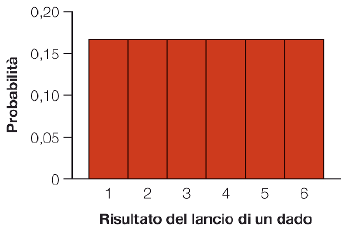
\includegraphics[width=0.35\textwidth]{fig5.4-1}
    \caption{\small{}}
\end{figure}

\section{Eventi indipendenti}
Due eventi si dicono \textbf{indipendenti} se il verificarsi di uno dei due non influenza in alcun modo la probabilità che si verifichi anche l'altro.

\section{Eventi incompatibili}
Quando due eventi sono indipendenti e mutualmente esclusivi, ovvero non possono verificarsi simultaneamente, si parla di \textbf{eventi incompatibili}. Per esempio, un singolo dado lanciato una sola volta non può presentare simultaneamente sia 1 che 6: gli eventi "1" e "6" sono incompatibili.
\\
In termini matematici, due eventi sono incompatibili se $Pr[A\ e\ B]=0$, in cui $Pr[A\ e\ B]$ significa la probabilità che si verifichi sia A che B.

\section{Somma delle probabilità}
Se gli eventi che si tenta di combinare sono incompatibili, allora il calcolo della probabilità che si verifichi l'uno o l'altro è semplicemente la somma delle probabilità per ciascuno di quegli eventi considerati separatamente. Ottenere 7 e ottenere 11 lanciando due dadi sono eventi incompatibili, perciò, la probabilità di ottenere 7 o 11 lanciando due dadi è la probabilità che esca 7 più la probabilità che esca 11: Pr[ottenere 7 o ottenere 11] = Pr[ottenere 7] + Pr[ottenere 11].
\\
Questa proprietà additiva delle probabilità di eventi incompatibili è detta \textbf{regola della somma} (un caso particolare del teorema della somma delle probabilità). 
\\
Dunque, secondo la regola della somma, se due eventi A e B sono incompatibili, allora: 
\begin{equation}
    Pr[A\ o\ B] = Pr[A] + Pr[B]
\end{equation}
La regola della somma può essere estesa a più di due eventi, purché essi siano tutti incompatibili.
\\
\\
La somma delle probabilità di tutti i possibili risultati incompatibili di una prova casuale deve essere uguale ad 1; ciò significa che la probabilità che un evento non si verifichi è semplicemente 1 meno la probabilità che si verifichi.
\\
\\
Se due eventi non sono incompatibili (non mutualmente esclusivi ma indipendenti), la probabilità che l'uno oppure l'altro evento possa verificarsi viene data dalla \textbf{regola della somma generalizzata}:
\begin{equation}
    Pr[A\ o\ B] = Pr[A] + Pr[B] - Pr[A\ e\ B]
\end{equation}\\
\begin{figure}[h]\label{fig5.5-2}
    \centering
    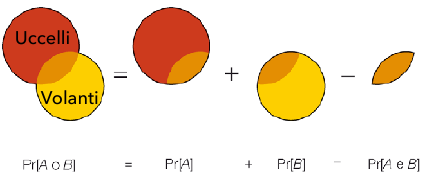
\includegraphics[width=0.6\textwidth]{fig5.5-2}
    \caption{\small{}}
\end{figure}

Se non si sottraesse la probabilità che si verifichino sia A che B, si conterrebbero due volte i risultati in cui gli eventi si verificano contemporaneamente.
In realtà, la regola potrebbe essere applicata anche a casi in cui si hanno eventi mutualmente esclusivi, \colorbox{lyellow}{perché}

\section{Diagrammi di Venn}
Un modo utile per ragionare sulle probabilità degli eventi è usare uno strumento grafico, detto \textbf{diagramma di Venn}. L'area del diagramma di Venn rappresenta tutti i risultati possibili di una prova casuale, e si possono rappresentare vari eventi come aree del diagramma. 
\\
Se il box per ciascun risultato ha la stessa area, i risultati sono equiprobabili.
Es. probabilità che, lanciando due dadi a 6 facce, si ottengano due numeri che, sommati, restituiscono un valore di 7 o di 11.
\\
La probabilità di ottenere 7 o 11 è additiva; in questo caso, la funzione di probabilità non è più uniforme, ma segue una curva a campana.
\\
Dunque, le probabilità di eventi alternativi ma non incompatibili sono additive.
\begin{figure}[h]\label{fig5.5-1}
    \centering
    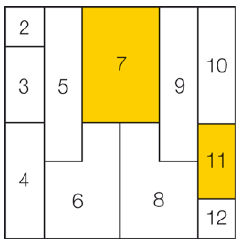
\includegraphics[width=0.6\textwidth]{fig5.5-1}
    \caption{\small{}}
\end{figure}
\begin{figure}[h]\label{istogrammaperdiagramma}
    \centering
    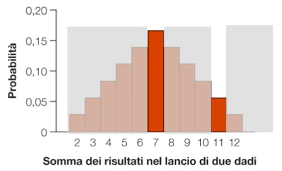
\includegraphics[width=0.6\textwidth]{istogrammaperdiagramma}
    \caption{\small{}}
\end{figure}

\section{Prodotto di probabilità\label{secprodottodiprobabilità}}
Quando due eventi sono indipendenti, la probabilità che si verifichino entrambi è data dal prodotto della probabilità del primo evento per la probabilità del secondo. Questa proprietà degli eventi indipendenti, detta regola del prodotto (un caso particolare del teorema della probabilità composta), è essenziale per l'analisi dei dati perché permette di determinare se due o più variabili siano associate.
\\
Secondo la regola del prodotto, se due eventi A e B sono indipendenti, allora:
\begin{equation}
    Pr[A\ e\ B] = Pr[A] x Pr[B] 
\end{equation}
La regola del prodotto riguarda combinazioni che implicano "e", cioè la probabilità che si verifichino entrambi gli eventi. Volendo conoscere la probabilità che si verifichino questo e quello, e se i due eventi sono indipendenti, possiamo moltiplicare le probabilità di ciascuno di essi per ottenere la probabilità che si verifichino entrambi.
\begin{figure}[h]\label{fig5.6-1}
    \centering
    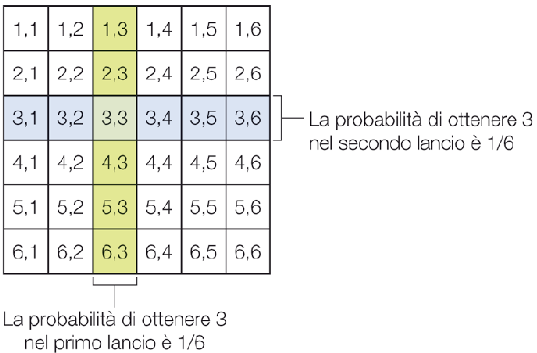
\includegraphics[width=0.6\textwidth]{fig5.6-1}
    \caption{\small{}}
\end{figure}
\\
\colorbox{lyellow}{\parbox{0.97\textwidth}{OPPURE
\\
La probabilità di ottenere due eventi indipendenti mutualmente esclusivi si ottiene invece calcolando il prodotto delle probabiltà dei singoli eventi.
\\
Es. probabilità che su due lanci esca 3 e 3.
\\
\\
Nel caso di eventi indipendenti non mutualmente esclusivi si calcola il prodotto dei due o più eventi per ottenere la probabilità della combinazione degli eventi considerati.}}
\begin{example}[slot machines]
    Con una slot machine si vince il 9.8\% delle volte ($Pr[vincita] = 0.098$), indipendentemente dalla giocata precedente.
    Qual è la probabilità che un giocatore perda 8 volte di seguito?
    \begin{equation}
        Pr[perdita] = 1 - Pr[vincita] = 0.902
    \end{equation}
    Vincita e perdita sono incompatibili, quindi:
    \begin{equation}
        Pr[8\ perdite] = Pr[perdita]^8 = 0.438
    \end{equation}
\end{example}

\section{Alberi di probabilità}
Un \textbf{albero di probabilità}, o albero probabilistico, è un diagramma che può essere utilizzato per calcolare le probabilità di combinazioni di eventi che sono i risultati di più prove casuali.

\section{Probabilità condizionata e teorema della probabilità totale}
La \textbf{probabilità condizionata} (o subordinata) è la probabilità di un evento condizionata dal verificarsi di un altro evento.
\\
La probabilità condizionata si indica come: Pr[evento|condizione] = probabilità.
Il che indica la probabilità che si verifichi l'evento quando la condizione è soddisfatta.
\\
La barra verticale al centro di questa espressione sta per "dato che" o "quando la condizione seguente è soddisfatta".
\\
Volendo conoscere la probabilità complessiva di un particolare evento, si devono sommare tutte le sue probabilità per ogni possibile condizione, pesate sulla probabilità di quella condizione. Questa regola è nota come \textbf{teorema della probabilità totale (o globale)}, secondo cui la probabilità di un evento X è:
\begin{equation}
    Pr[X] = \sum{Pr[Y_i]\ Pr[X | Y_i]}
\end{equation}

\section{Teorema della probabilità composta}
Le probabilità condizionate ci permettono di calcolare la probabilità di una combinazione di due eventi anche se essi non sono indipendenti. In questa situazione, possiamo valutare la probabilità che si verifichino entrambi moltiplicando la probabilità di un evento per la probabilità condizionata dell'altro evento, ovvero per la probabilità dell'altro evento condizionata al verificarsi del primo evento. Si tratta della regola del prodotto generalizzata, detta anche \textbf{teorema della probabilità composta}. 
\\
La regola del prodotto generalizzata permette di trovare la probabilità che si verifichino due eventi anche quando sono dipendenti: 
\begin{equation}
    Pr[A\ e\ B] = Pr[A] Pr[B|A]
\end{equation}
Riflettendo attentamente, possiamo renderci conto di come questa regola sia ragionevole. Affinché due eventi (A e B) si verifichino, deve verificarsi l'evento A. Per definizione, ciò avviene con probabilità Pr[A]. Sapendo che A si è verificato, la probabilità che si verifichi anche B è Pr[B|A]. Moltiplicando tra loro queste probabilità otteniamo la probabilità che si verifichino sia A sia B.
\\
Vale anche l'inverso:
\begin{equation}
    Pr[A\ e\ B] = Pr[B] Pr[A|B]
\end{equation}
Dunque, il teorema della probabilità composta è applicabile anche ad eventi non indipendenti ed è simmetrico.

\begin{example}[\textit{Nasonia vitripennis}]
    La vespa parassita Nasonia vitripennis depone uova in larve di mosca decidendone il sesso in base a se la larva è già parassitata (90\% maschi perché questi riusciranno a fecondare tutte le uova delle altre femmine competendo bene con i maschi dell'altra parassitazione) o no (soprattutto femmine e pochi maschi perché questi pochi potrebbero fecondare tutte le femmine). In questi casi la probabilità di parassitosi è dello 0.2 (assumendo che questa sia la stessa per larve già parassitate e non). Il problema può essere rappresentato mediante diagramma di Venn (in questo caso molto simile ad un mosaic plot) o albero delle probabilità. 
    \\
    Qual è la probabilità che un uovo sia maschio? Sommando le due probabilità relative:
    \begin{equation}
        \begin{gathered}
            Pr[M]=Pr[ospite\ parassitato]\ Pr[M|ospite\ parassitato]\ + \\ +\ Pr[ospite\ non\ parassitato]\ Pr[M|ospite\ non\ parassitato]
        \end{gathered}
    \end{equation}
\end{example}
\clearpage
\begin{figure}[h]\label{fig5.8-1}
    \centering
    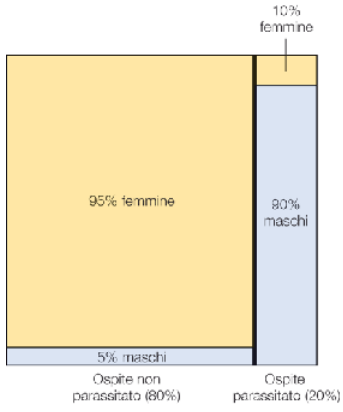
\includegraphics[width=0.6\textwidth]{fig5.8-1}
    \caption{\small{}}
\end{figure}
\begin{figure}[h]\label{alberoprobabilità}
    \centering
    \includegraphics[width=0.6\textwidth]{alberoprobabilità}
    \caption{\small{}}
\end{figure}
 
\section{Teorema di Bayes}
Partendo dalla regola del prodotto generalizzata, dato che:
\begin{equation}
    Pr[A\ e\ B] = Pr[A]\ Pr[B|A] 
\end{equation}
E che:
\begin{equation}
    Pr[B\ e\ A] = Pr[B]\ Pr[A|B] 
\end{equation}
Allora è anche vero che:
\begin{equation}
    Pr[B] * Pr[A|B] = Pr[A]\ Pr[B|A] 
\end{equation}
Dividendo entrambi i membri per $Pr[B]$ si ottiene il \textbf{teorema di Bayes} (sostituire E con B):
\begin{equation}
    Pr[A|B] = \frac{Pr[B|A]\ Pr[A]}{Pr[B]}
\end{equation}
Ovvero: la probabilità di un evento, dato un altro evento che la condiziona, è uguale alla probabilità dell'evento per la probabilità dell'evento che lo condiziona, dato l'evento iniziale, diviso la probabilità dell'evento che lo condiziona.
\begin{example}[sindrome di Down]
    La prevalenza (frequenza di casi che si ha su un certo numero di eventi) della sindrome di Down è di $\frac{1}{1000}$ ($Pr[DS] = \frac{1}{1000} = 0.001$) feti.
    \\
    L'amniocentesi porta ad aborto in $\frac{1}{200}$.
    \\
    Il Triplo Test (TT) è un'alternativa all'amniocentesi che ha una sensitività (probabilità di rilevare un vero positivo) di 0.6 (60\% dei casi rileva un feto con DS, Pr[TTpos | DS] = 0.6), e 0.05 della probabilità di avere un falso positivo (5\% di avere un falso positivo).
    \\
    Qual è la probabilità che si abbia un vero positivo quando si ottiene un TT positivo (Pr[DS | TTpos])?
    \\
    \\
    Applicando il teorema di Bayes:
    \begin{equation}
        Pr[TTpos] = Pr[TTpos | DS]\ Pr[DS] + Pr[TTpos | no\ DS]\ Pr[no\ DS] = 0.05055
    \end{equation}
    \begin{equation}
        Pr[DS | TTpos] = \frac{Pr[DS]\ Pr[TTpos | DS]}{Pr[TTpos]}= 0.012
    \end{equation}
\end{example}

\chapter{Test delle ipotesi}\footnote{Capitolo 6, Whitlock and Schluter, Analisi statistica dei dati biologici (2010)}
\\
Una teoria non confutabile non è necessariamente falsa, ma non rientra nell'ambito scientifico, bensì in quello metafisico.
\\
Il neopositivismo impiega il criterio di verificabilità: per essere corretta, una teoria deve essere verificata, il che può essere fatto mediante la logica.
\\
Non potendo fare esperienza dell'universale si deve adottare l'\textbf{approccio falsificazionista}: bisogna provare che un'ipotesi sia sbagliata per smentirla.
\\
Un'ipotesi non si verifica e non si può accettare, si possono portare prove a suo sostegno e si può falsificare.
\begin{example}[sesso e altezza]
    Data un'altezza media dei maschi pari ad $\overline{y}_m = 175.6\ cm$, con deviazione standard $s_m= 7.1$, ed un'altezza media delle femmine pari ad $\overline{y}_f = 162.6\ cm$, con deviazione standard $s_f= 6.4$, i maschi sono davvero più alti delle femmine?
    \\
    Un valore di 193 cm quanto è anomalo nella popolazione maschile?
    \begin{equation}
        193-175.6/7.1 = 2.qualcosa
    \end{equation} 
    Dunque, dato che soglia oltre la quale si ha solo il 5\% dei casi, avere 193 è solo in meno del 5\% dei casi.
    \\
    (stessa cosa per femmine e 155 cm?)
\end{example}
\clearpage
\section{Ragionamento logico}
Il ragionamento scientifico può seguire percorsi alternativi:
\begin{table}[h]
    \centering
    \renewcommand\arraystretch{1.2}
    \begin{tabular}{ c|c|c }
    \hline
    \textbf{Deduzione} & \makecell[l]{Dall'universale al particolare\\ attraverso postulati\\ e concatenazioni logiche\\ (conseguente).} & \makecell[l]{\textbf{Regola}: tutti i fagioli di questo\\ sacchetto sono bianchi\\
    \textbf{Caso}: questi fagioli vengono\\ da questo sacchetto\\
    \textbf{Risultato}: questi fagioli sono bianchi}\\
    \hline
    \textbf{Induzione} & \makecell[l]{Dal particolare all'universale\\ attraverso osservazioni ripetute\\ (non sempre conseguente).} & \makecell[l]{\textbf{Caso}: questi fagioli vengono\\ da questo sacchetto\\
    \textbf{Risultato}: questi fagioli sono bianchi\\
    \textbf{Regola}: tutti i fagioli di questo\\ sacchetto sono bianchi}\\
    \hline
    \textbf{Abduzione} & \makecell[l]{Dal particolare all'universale,\\ si tratta più di intuito\\ che di reale logica\\ (non sempre conseguente).} & \makecell[l]{\textbf{Risultato}: questi fagioli sono bianchi\\
    \textbf{Regola}: tutti i fagioli di questo\\ sacchetto sono bianchi\\
    \textbf{Caso}: questi fagioli vengono da questo\\ sacchetto
(non è assolutamente detto)}\\
    \hline
    \end{tabular}
    \caption{}
    \label{tabragionamentologico}
\end{table}\noindent

\section{Metodo scientifico galileiano}
Il metodo scientifico si basa su una combinazione di processi induttivi e deduttivi; può essere infatti scomposto in due fasi:
\begin{itemize} \tightlist
    \item \textbf{induttiva} (dal particolare all'universale):
    \begin{itemize} \tightlist
        \item osservazione;
        \item formulazione di ipotesi;
    \end{itemize}
    \item \textbf{deduttiva} (dall'universale al particolare):
    \begin{itemize} \tightlist
        \item formulazione della teoria e dimostrazione matematica;
        \item verifica sperimentale.
    \end{itemize}
\end{itemize}

\section{Formulazione delle ipotesi}
Per formulare un'ipotesi biologica bisogna definire:
\begin{itemize} \tightlist
    \item \textbf{enunciato} chiaro e specifico;
    \item \textbf{razionale}, ciò che giustifichi l'ipotesi nella sua formulazione (alla fine dell'introduzione si elencano le ipotesi, il razionale si evince dal resto dell'introduzione);
    \item \textbf{previsione}, che deve essere precisa e misurabile.
\end{itemize}

\section{Verifica delle ipotesi}
La verifica formale delle ipotesi parte dall'enunciazione chiara di due ipotesi, l'ipotesi nulla e l'ipotesi alternativa, riguardo a un parametro della popolazione. L'ipotesi nulla si può considerare l'ipotesi di base, di partenza, mentre l'ipotesi alternativa comprende in genere ogni altra possibilità rispetto a quelle enunciate nell'ipotesi nulla. 
\\
\\
L'\textbf{ipotesi nulla} è un enunciato specifico riguardo al valore di un parametro della popolazione. Viene formulata ai fini del ragionamento e include spesso il punto di vista scettico. L'ipotesi nulla spesso afferma che un parametro nella popolazione di interesse è pari a zero (cioè, nessun effetto, nessuna preferenza, nessuna correlazione o nessuna differenza). In generale, questa ipotesi è un enunciato che sarebbe interessante rifiutare. L'ipotesi nulla, chiamata anche ipotesi zero, o semplicemente H-zero, e indicata con il simbolo $H_0$, è sempre specifica: identifica un particolare valore del parametro studiato. 
\\
\\
Ogni ipotesi nulla è associata a un'\textbf{ipotesi alternativa} ($H_A$) che generalmente rappresenta tutti gli altri valori possibili di un parametro rispetto a quelli previsti nel ipotesi nulla.
\\
Per questo motivo spesso coincide, ma non sempre, con l'ipotesi che il ricercatore spera essere vera.
\\
A differenza dell'ipotesi nulla, l'ipotesi alternativa non è specifica. Essa include ogni valore possibile per una caratteristica della popolazione o per una differenza tra popolazioni, eccettuato il valore specificato dall'ipotesi nulla.
\\
L'ipotesi alternativa può essere a una o due code: a una coda se è accettabile solo il cambiamento in una delle due direzioni, a due code se vanno bene entrambe le direzioni.
\\
Se un'ipotesi alternativa sia ad \textbf{una} o \textbf{due code} si deve decidere a priori e la decisione deve essere supportata da un forte razionale.
\\
\\
L'ipotesi nulla è l'unica ipotesi con la quale vengono effettivamente messi alla prova i dati. Se i dati sono compatibili con l'ipotesi nulla, allora diciamo che non possiamo rifiutarla (non "accettiamo" mai l'ipotesi nulla). Se i dati sono invece incompatibili, la scartiamo e accettiamo l'ipotesi alternativa. Rifiutare $H_0$, significa escludere il valore che H0 specifica. Il rifiuto dice anche in quale direzione si trova verosimilmente il valore vero rispetto a quello specificato dall'ipotesi nulla, senza però suggerire nulla sul valore numerico del parametro della popolazione. Per stimare i valori dei parametri e il loro errore usiamo il processo di stima.
\begin{example}[lateralità nei rospi]\label{eslateralita}
    Gli esseri umani sono in prevalenza destrimani. Questa lateralità è presente anche in altri animali? Bisazza et al. (1996) hanno studiato a tal proposito il rospo comune (\textit{Bufo bufo}), campionando 18 rospi selvatici e sottopo- nendoli a un esperimento. Assumiamo prima di tutto che il campione fosse casuale. I rospi furono trasferiti in laboratorio e furono sottoposti, uno alla volta, alla stessa umiliazione: venne avvolto un palloncino attorno alla testa di ogni individuo. Poi i ricercatori registrarono quale dei due arti anteriori ogni rospo usava per togliersi il palloncino dalla testa, trovando che ogni rospo tendeva a usare uno più dell'altro. A questo punto ricercatori si chiesero: i rospi destrimani e quelli mancini sono presenti con uguale frequenza nella popolazione dei rospi, oppure uno dei due tipi di lateralità è più frequente dell'altro, come nell'uomo? Dei 18 rospi sottopo- sti al test, 14 erano destrimani e 4 erano mancini. Questi risultati si possono con- siderare una chiara I'evidenza che nei rospi uno dei due tipi di lateralità prevale sull'altro?
    \\
    \\
    Il valore numerico di interesse è la frazione di rospi destrimani nella popolazione. Chiamiamo p questa proporzione. Secondo l'ipotesi di partenza ($H_0$), i rospi mancini e quelli destrimani sono ugualmente frequenti nella popolazione ($p=0.5$). 
    Se l'ipotesi nulla è falsa, allora nei rospi prevale l'utilizzo di una zampa, dunque, secondo HA, i rospi mancini e quelli destrimani non sono ugualmente frequenti nella popolazione ($p \neq 0.5$).
    \\
    \\
    L'ipotesi alternativa è bilaterale (o a due code). Ciò significa semplicemente che essa contempla due possibilità: che p sia maggiore di 0,5 (i rospi destrimani sono più frequenti di quelli mancini nella popolazione) oppure che p sia minore di 0,5 (i rospi mancini predominano). Nessuna delle due possibilità può essere esclusa prima dell'esperimento, quindi entrambe devono essere incluse nell'ipotesi alternativa. In un test bilaterale (o test a due code), l'ipotesi alternativa include valori da entrambi i lati (maggiori e minori) del valore specificato dall'ipotesi nulla. La definizione "bilaterale" deriva dal fatto che l'ipotesi alternativa contiene valori da entrambe le parti rispetto al valore specificato dall'ipotesi nulla, mentre la definizione "a due code" si riferisce alle code della distribuzione campionaria, dove una "coda" è la regione all'estremità superiore o all'estremità inferiore della distribuzione. 
\end{example}

\section{Statistica test}
La \textbf{statistica test} è una grandezza, calcolata sulla base del dati osservati, che viene utilizzata per valutare il grado di compatibilità dei risultati con il risultato che ci aspettiamo se fosse vera l'ipotesi nulla.
\\
Serve una statistica test che rappresenti la previsione per verificare le ipotesi.
\\
Nello studio sui rospi usiamo come statistica test il numero osservato di rospi destrimani. 
\\
\\
Purtroppo non sempre i dati rispecchiano perfettamente la realtà. A causa degli effetti del caso durante il campionamento, non ci attendiamo di osservare esattamente 9 rospi destrimani quando campioniamo 18 rospi dalla popolazione, anche quando l'ipotesi nulla è vera. Anche in questo caso, infatti, esiste generalmente una discrepanza, dovuta al caso, tra il risultato osservato e quello atteso. Questa discrepanza può essere piuttosto grande, pur essendo H0 vera, in particolare se i dati non sono molto numerosi. Per decidere se i dati siano compatibili con l'ipotesi nulla, dobbiamo calcolare la probabilità di un disaccordo tanto ampio quanto quello osservato, assumendo che l'ipotesi nulla sia vera.
\\
Per ottenere questa probabilità dobbiamo determinare la distribuzione campionaria della statistica test assumendo che l'ipotesi nulla sia vera. Dobbiamo cioè determinare i valori della statistica test che sono possibili sotto l'ipotesi nulla e le probabilità a essi associate. La distribuzione di probabilità dei valori della statistica test quando si assume che l'ipotesi nulla sia vera è detta "distribuzione campionaria sotto H0" o, più semplicemente, distribuzione nulla. 
\\
La distribuzione nulla è la distribuzione campionaria dei possibili valori che può assumere una statistica test quando si ipotizza che sia vera l'ipotesi nulla.
\\
Analizzando questa distribuzione, possiamo concludere che ogni numero di rospi destrimani tra 0 e 18 può essere osservato in un campione casuale di 18 individui quando è vera $H_0$, ma alcuni valori sono molto più probabili di altri.

\section{Livello di significatività di P}
II metodo comunemente utilizzato per descrivere il disaccordo tra i dati e un'ipotesi nulla è calcolare la probabilità di ottenere quei dati, oppure di ottenere i dati che sono ancor più diversi da quelli attesi (cioè meno probabili), assumendo vera l'ipotesi nulla. In altre parole, vogliamo conoscere la probabilità complessiva, se fosse vera $H_0$, di tutti i risultati ugualmente insoliti o piiù insoliti rispetto a quelli osservati. Se questa probabilità risulterà piccola, allora l'ipotesi nulla verrà considerata incompatibile con i dati e verrà rifiutata in favore dell'ipotesi alternativa. Se questa probabilità non risulterà piccola, allora sarebbe ingiustificato mettere in dubbio l'ipotesi nulla, che quindi non verrà rifiutata. La probabilità di ottenere i dati osservati, o i dati che sono ancor meno in accordo con l'ipotesi nulla, assumendo che sia vera l'ipotesi nulla, è detta \textbf{P-value} (o valore P). Se il P-value è piccolo, allora l'ipotesi nulla è incompatibile con i dati e la rifiutiamo. Altrimenti essa non può essere rifiutata.
\\
Il P-value (o valore P) è la probabilità di ottenere i dati osservati (oppure i dati che hanno una differenza altrettanto grande o ancora maggiore rispetto al valore dell'ipotesi nulla) se l'ipotesi nulla fosse vera (ovvero per caso). In pratica, calcoliamo il P-value in base alla distribuzione nulla della statistica test.
\\
\\
\colorbox{lyellow}{\parbox{0.98\textwidth}{
    P, riferito ad una curva di distribuzione di frequenza, rappresenta la probabilità di osservare per caso un valore uguale o più o meno estremo di quello che si osserva (quindi quanto è probabile il valore della statistica test se l'ipotesi nulla è vera). Se $P>0.05$ (test non significativo, la differenza osservata potrebbe essere semplicemente dovuta alla variabilità naturale o campionaria, non si può escludere che siano dovute al caso) non si può rifiutare l'ipotesi nulla e supportare l'ipotesi alternativa. Se $P \le 0.05$ (test significativo *) allora si rifiuta l'ipotesi nulla e si supporta quella alternativa, a maggior ragione se $P \le 0.01$ (test molto significativo **) o 0.001 (test altamente significativo ***); questi tre livelli sono standard internazionali. (la differenza osservata è difficilmente osservabile per caso).}}
\\
\\
I valori soglia con cui si confronta il p-value sono indicati con $\alpha$ (0.05 = meno di 5 volte su 100 si potrebbero trovare valori della statistica test uguali o più estremi, 0.01, 0.001).
\\
\\
La nostra ipotesi alternativa $H_A$ è bilaterale, quindi dobbiamo considerare nel calcolo del P-value i risultati tanto insoliti quanto i dati osservati, ho ancora più insoliti, localizzati su entrambe le code della distribuzione.
\\
La probabilità di avere 14 o più rospi destrimani, sotto $H_0$, è pari a:
\begin{equation}
    Pr[\ge 14\ destrimani] = Pr[14] + Pr[15] + Pr[16] + Pr[17] + Pr[18] = 0,0155 
\end{equation}
In cui $Pr[14]$ è la probabilità di osservare esattamente 14 rospi destrimani. Le probabilità relative a 14, 15, 16, 17 e 18 rospi destrimani possono essere sommate perché i singoli risultati sono tra di loro incompatibili (cioè mutuamente esclusivi). Questa somma non è però il P-value, perché non include ancora i risultati altrettanto estremi giacenti sulla coda sinistra della distribuzione nulla (quelli cioè che implicano una predominanza di rospi mancini). Il metodo più rapido per includere le probabilità dei risultati ugualmente estremi localizzati sull'altra coda della distribuzione è moltiplicare per 2 la somma precedente, ottenendo il P-value desiderato. In altre parole, se assumiamo che l'ipotesi nulla sia vera, la probabilità di un risultato tanto estremo quanto "14 rospi destrimani osservati su 18 campionati", o ancora più estremo, è pari a $P = 0,031$. 
\\
\\
Se il P-value è "piccolo" rifiutiamo l'ipotesi nulla; altrimenti, non la rifiutiamo. Per convenzione, nella maggior parte dei settori della ricerca biologica il confine tra P-value piccoli e P-value non piccoli è 0,05. In altre parole, se $P< 0,05$ rifiutiamo l'ipotesi nulla, mentre se $P> 0,05$ non la rifiutiamo.
\\
Il P-value per i dati sui rospi, $P= 0,031$, è in effetti minore di 0,05: rifiutiamo quindi l'ipotesi nulla per la quale i rospi mancini e quelli destrimani sono ugualmente frequenti nella popolazione di rospi. In base a questi dati possiamo concludere che la maggioranza di rospi nella popolazione è destrimane.
\\
Questa soglia di decisione per P (cioè, $P= 0,05$) è detta livello di significatività, e si indica con $\alpha$. In biologia, il livello di significatività più usato è $\alpha = 0,05$, ma potrete incontrare alcuni studi che usano un differente valore di $\alpha$. Dopo 0.05, il successivo livello di significatività più utilizzato è 0,01.
\\
\\
Quando si devono comunicare i risultati di uno studio con un articolo scientifico o una relazione, è necessario includere sempre il valore della statistica test, la dimensione campionaria ed il P-value. Inoltre, è sempre utile fornire gli intervalli di confidenza, o almeno gli errori standard, per i parametri di interesse.
\begin{example}[voti in biostatistica]\label{esvoti}
    Le ipotesi sono:
    \begin{itemize} \tightlist
        \item $H_0$: medie di ragazzi e ragazze in biostatistica sono uguali;
        \item $H_{A1}$: ragazze hanno voti più alti in biostatistica dei ragazzi;
        \item $H_{A2}$: ragazzi hanno voti più alti in biostatistica delle ragazze.
    \end{itemize}
    Bisogna confrontare le medie di ragazze e ragazzi; la statistica test in questo caso è il calcolo della differenza tra le medie: se $H_0$ è verificata, la differenza è pari a zero o quasi (si deve considerare la dispersione, generata dalla variabilità insita nella popolazione e dalla dimensione del campione).
    \begin{equation}
        \frac{\overline{Y}_F-\overline{Y}_M}{ES_{\overline{Y}_F-\overline{Y}_M}}
    \end{equation}
\end{example}

\section{Errori nella verifica delle ipotesi}
Rifiutare $H_0$ non significa necessariamente che l'ipotesi nulla sia falsa. 
\\
Analogamente, il mancato rifiuto di $H_0$, non significa necessariamente che l'ipotesi nulla sia vera. Le ipotesi riguardano infatti le popolazioni, ma avendo a disposizione solo l'informazione contenuta nei campioni, che sono inevitabilmente influenzati dal caso, è possibile che una conclusione sulle ipotesi sia errata. 
\\
Ovviamente non saremo in grado di dire, dopo aver quantificato il P-value e deciso se rifiutare o no l'ipotesi nulla, se abbiamo commesso un errore. È possibile, però, ragionare sugli errori e in parte quantificarli se i dati provengono da un campione casuale, valutando quindi con maggiore consapevolezza la decisione finale. 
\\
\\
Quando si rifiuta un'ipotesi nulla vera, si commette un \textbf{errore di tipo I}. Se invece non si rifiuta un'ipotesi nulla falsa, allora si commette un \textbf{errore di tipo II}. 
\\
Il livello di significatività a corrisponde alla probabilità di commettere un errore di tipo I. Se seguiamo la convenzione e usiamo un livello di significatività 0.05, allora dobbiamo ritiutare $H_0$ quando $P$ è inferiore o uguale a 0,05. Ciò significa che, se l'ipotesi nulla fosse vera, la rifiuteremmo erroneamente 1 volta su 20. I biologi considerano accettabile il rischio di commettere un errore di primo tipo. 
\\
Si potrebbe ridurre il tasso di errore di tipo I usando un livello di significatività inferiore a 0.05. Tuttavia, questa scelta avrebbe anche l'effetto collaterale di aumentare la probabilità di commettere un errore di tipo II. Ridurre $\alpha$ rende più difficile rifiutare l'ipotesi nulla quando è vera, ma rende anche più difficile rifiutarla quando è falsa. Questo è un motivo per cui si usa per convenzione 0.05.
\\
Il mancato rifiuto di un ipotesi nulla falsa è un errore di tipo II.
\\
Se in un certo studio, applicando una certa statistica, la probabilità di commettere un errore di tipo II è bassa, si dice che il test ha un'elevata potenza. La \textbf{potenza} è la probabilità che un campione casuale estratto da una popolazione, quando viene analizzato, determini il rifiuto di un ipotesi nulla falsa.
\begin{equation}
    potenza\ del\ test = 1-\beta
\end{equation}
A parità di tutti gli altri fattori, un test è migliore se ha una potenza più elevata.
\\
Poiché non si conosce mai il valore vero, non si è in grado di prevedere con precisione la potenza del test utilizzato in uno studio. 
\\
Quando però si è in grado di fare qualche previsione, anche approssimativa, sull'entità della possibile deviazione dalle ipotesi nulla, allora si può stimare la potenza. In generale, un test ha una potenza maggiore se la dimensione campionaria è grande, se la discrepanza vera dalle ipotesi nulla è grande e se la variabilità della popolazione è bassa.
\\
Si vuole solitamente una potenza di almeno 0.8 e quindi un $\beta$ di 0.2.
\begin{figure}[h]\label{erroriverificaipotesi}
    \centering
    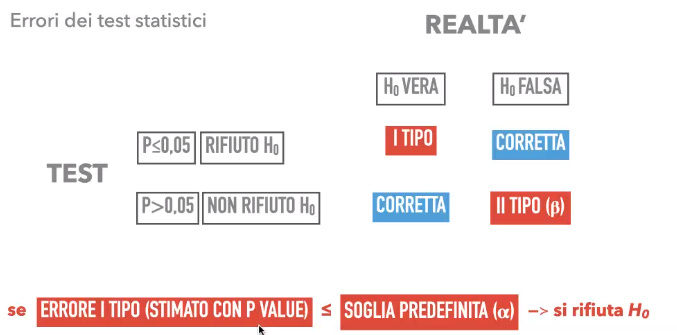
\includegraphics[width=0.6\textwidth]{erroriverificaipotesi}
    \caption{\small{}}
\end{figure}
\begin{example}[fiori sinistrorsi]
    Essere sinistrorsi o destrorsi per quanto riguarda la posizione dei pistilli di alcuni fiori è determinato da un fenomeno di dominanza genetica.
    \\
    Si è visto che:
    \begin{itemize} \tightlist
        \item da un incorcio di puri destrorsi e sinistrorsi si ottengono solo destrorsi (ds);
        \item dall'incrocio dell'F1 si ottengono 6 sinistrorsi (ss) e 21 ds.
    \end{itemize}
    Questo è coerente con quanto ci si aspetterebbe ($H_0$: 1 ss ogni 3 ds, come ci si aspetterebbe dalla teoria classica (0.25 della probabilità di ottenere ss)?
    \begin{figure}[H]\label{fig6.4-1}
    \centering
    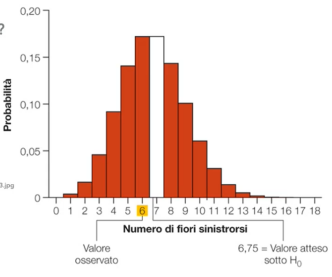
\includegraphics[width=0.6\textwidth]{fig6.4-1}
    \caption{\small{}}
    \end{figure}
In questo caso, la statistica test è la frazione di fiori ss trovata, che va confrontata con la distribuzione attesa, per vedere quanto sia frequente ottenere i valori ottenuti.
\\
Il valore atteso di fiori ss sulla base dell $H_0$ è 6.75, mentre il valore osservato è 6.
\\
Il p-value è rappresentato, nel grafico, da tutte le barre rosse, che rappresentano i valori uguali a 6 o più estremi, dunque il p-value è abbastanza coerente con la $H_0$.
\\
Dunque non si rifiuta l'ipotesi nulla.
\end{example}
\clearpage
\begin{example}[riconoscimento della paternità]
    18 prove indipendenti: soggetti diversi con foto diversi.
    Le ipotesi sono:
    \begin{itemize} \tightlist
        \item $H_0$: è impossibile attribuire ad un uomo la paternità di una figlia guardando foto dei due;
        \item $H_A$: è possibile.
    \end{itemize}
    Potrebbe essere un test ad una coda nel caso in cui la relazione padre-figlia potesse rendere sia più somiglianti che meno somiglianti, mentre nella realtà si tratta di un test ad una coda, poiché la relazione padre-figlia può rendere i due soggetti solo più somiglianti, e dunque potrebbe essere plausibile che l'osservatore riesca a riconoscere la relazione guardando le due foto, e dunque che il numero di risposte corrette sia più alto di quello che ci si aspetterebbe se l'$H_0$ fosse vera, mentre non è possibile che l'osservatore sbagli nell'indovinare la parentela significativamente di più di quanto ci si aspetti per caso.
    \begin{figure}[H]\label{fig6.5-1}
    \centering
    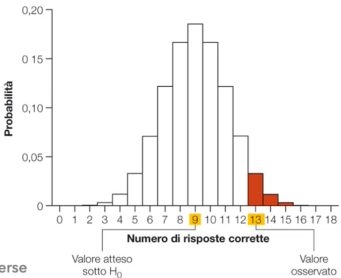
\includegraphics[width=0.6\textwidth]{fig6.5-1}
    \caption{\small{}}
    \end{figure}
    Con un P-value pari a 0.048 si rifiuta l'$H_0$, poiché il risultato ottenuto è significativamente diverso da ciò che ci si aspetterebbe se $H_0$ fosse vera, almeno prendendo in considerazione un valore di $\alpha$ pari a 0.05.
\end{example}

\part{Confronti tra gruppi}


\chapter{Analisi delle proporzioni (B5)}\footnote{Capitolo 7, Whitlock and Schluter, Analisi statistica dei dati biologici (2010)}

\section{Distribuzione binomiale}
Una misurazione effettuata su degli individui suddivide questi ultimi in due gruppi mutualmente esclusivi in base ad una certa caratteristica come, ad esempio, "successo" ed "insuccesso".
\\
Nella popolazione, una proporzione fissa "p" di individui rientra in uno dei due gruppi, mentre i restanti rientrano nell'altro gruppo.
\\
Se si estrae un campione casuale di n individui a partire dalla popolazione, la distribuzione campionaria del numero di individui che rientrano nella categoria "successo" è descritta dalla \textbf{distribuzione binomiale} (binomiale perché esistono soltanto due risultati possibili ed entrambi sono categorie con un certo nome).
\\
La distribuzione binomiale fornisce la distribuzione di probabilità di X successi in (1) un numero fisso (n) di prove (2) indipendenti (l'una dalle altre) quando (3) la probabilità di successo (p) è la stessa in ogni prova ed (4) i possibili risultati della prova sono solamente due:
\begin{equation}
P[X \ successi] = \binom{n}{X} \ p^X \ (1 - p)^{n-X}
\end{equation}
Il termine $\binom{n}{X}$ è detto \textbf{coefficiente binomiale}, e corrisponde al numero di combinazioni semplici di n elementi presi X alla volta; tale termine rappresenta il numero di sequenze ordinate uniche (diverse tra loro) di successi ed insuccessi che portano esattamente ad X successi in n prove, e sta per:
\begin{equation}
\binom{n}{X} = \frac{n!}{X!\ (n - X)!}
\end{equation}
In cui n! (n fattoriale) sta per:
\begin{equation}
n! = n\times (n-1)\times (n-3)\times ...\times 2\times 1
\end{equation}

\begin{example}[Fiori sinistrorsi]
In una popolazione di una specie floristica, p = 0.25 ha fiori sinistrorsi e 1-p = 0.75 ha fiori destrorsi. Con questa situazione si può usare la distribuzione binomiale per determinare la probabilità di ogni dato numero di successi (es. X = 6, con n = 27, ovvero con 27 fiori campionati):
\begin{equation}
P[6 \ fiori \ sinistrorsi] = \binom{27}{6} \ 0.25^6 \ (0.75)^{27-6} = 0.1719
\end{equation}
Dunque, esiste una probabilità di circa il 17\% che 6 fiori su 27 siano sinistrorsi, se la proporzione di fiori sinistrorsi nella popolazione è pari a 0.25.
\\
Si possono calcolare le probabilità associate ad ogni possibile numero di successi (in questo caso, da 0 a 27), e la distribuzione di probabilità così ottenuta si può riportare graficamente:
    \begin{figure}[H]\label{fig7.1-1}
    \centering
    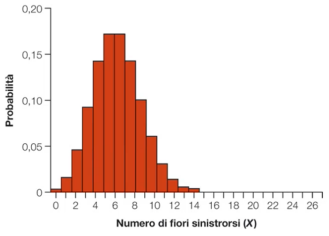
\includegraphics[width=0.6\textwidth]{fig7.1-1}
    \caption{\small{}}
    \end{figure}
Una distribuzione estremamente simile si può ottenere estraendo un gran numero di campioni casuali di n fisso (27, in questo caso), anche se la distribuzione binomiale fornisce probabilità più esatte, mentre le simulazioni ne forniscono di approssimate, sopratutto per n insufficienti; per verificare le ipotesi nulle si possono quindi utilizzare le distribuzioni binomiali.
\end{example}

\subsection{Distribuzione campionaria di una proporzione}
La proporzione di successi in una popolazione (X/n, X su n) si indica con p, mentre la proporzione di successi in un campione, ovvero la \textbf{proporzione campionaria}, si indica con $\hat{p}$ (p hat).
\\
La proporzione di successi in campioni casuali è uguale \textit{in media} alla proporzione di successi nella popolazione: $\hat{p}$ è quindi una stima non distorta della proporzione nella popolazione perché fornisce, in media, la risposta corretta.
\\
\\
Come si nota in Figura \ref*{fig7.1-2}, la dimensione campionaria influisce sulla larghezza della distribuzione campionaria di $\hat{p}$.\\
Quando n è grande, la distribuzione campionaria è stretta. Questo effetto è quantificato dall'\textbf{errore standard di $\hat{p}$}:
\begin{equation}
\sigma_{\hat{p}} = \sqrt{\frac{p(1-p)}{n}}
\end{equation}
\label{devstphat}
Campioni di grandi dimensioni ottenuti campionando più volte una stessa popolazione avranno proporzioni stimate più vicine tra loro e più vicine alla proporzione nella popolazione, rispetto ai campioni piccoli: i campioni più grandi forniscono dunque stime più precise (\textbf{legge dei grandi numeri}).
\clearpage
\begin{figure}[h]\label{fig7.1-2}
    \centering
    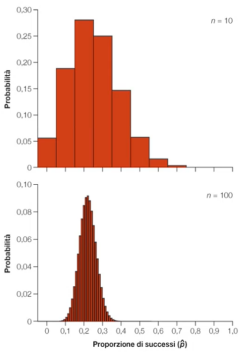
\includegraphics[width=0.6\textwidth]{fig7.1-2}
    \caption{\small{}}
\end{figure}

\section{Studio di una proporzione: il test binomiale}

Il \textbf{test binomiale} viene usato nella verifica delle ipotesi quando una variabile in una popolazione ha due stati possibili (successo, insuccesso) e si vuole verificare se la frequenza relativa di successi nella popolazione (p) sia pari al valore atteso assumendo vera l'ipotesi nulla ($p_0$).
\\
Le ipotesi nulla ed alternativa assumono particolari forme:
\begin{itemize} \tightlist
\item $H_0$: la frequenza relativa di successi nella popolazione è $p_0$;
\item $H_A$: la frequenza relativa di successi nella popolazione è diversa da $p_=$.
\end{itemize}
Il valore atteso sotto l'ipotesi nulla può essere dato da una qualsiasi proporzione compresa tra 0 ed 1, estremi inclusi.

\begin{example}[sesso e cromosoma X]
    Si vuole provare che i geni legati alla spermatogenesi si trovino preferenzialmente sul cromosoma X.
    \\
    Su 25 geni campionati, 10 (40\%) risiedono effettivamente sul cromosoma X.
    \\
    Se i geni per la spermatogenesi fossero distribuiti casualmente nel genoma, solo il 6.1\% di essi risiederebbe sul cromosoma X, poiché su tale cromosoma è presente solo il 6.1\% del genoma.
    \\
    Definiamo le ipotesi:
    \begin{itemize} \tightlist
    \item $H_0$: la probabilità che un gene per la spermatogenesi risieda sul cromosoma X è pari a 0.061 ($p_0 = 0.061$);
    \item $H_A$: la probabilità che un gene per la spermatogenesi risieda sul cromosoma X è diversa da 0.061 ($p\ne 0.061$).
    \end{itemize}
    In questo caso, dato che è teoricamente possibile che i geni per la spermatogenesi risiedano meno sul cromosoma X che su altre parti del genoma, l'ipotesi alternativa prevede tutti i casi in cui la probabilità è diversa da 0.061, sia quelli in cui la probabilità eccede tale valore, sia quelli in cui essa ne è minore; pertanto, in questo caso, il test è a due code.
    \\
    Nel caso del test binomiale, la statistica test utile per confrontare il risultato osservato con quello atteso sotto l'ipotesi nulla è il numero di successi osservato; in questo caso, dunque, la statistica test assume il valore di 10 (10 geni per la spermatogenesi osservati sul cromosoma X). Il valore atteso sotto l'ipotesi nulla è invece $0.061 x 25 = 1.525$. Dunque, nel campione, il numero di geni per la spermatogenesi osservati sul cromosoma X è maggiore di quello atteso sotto l'ipotesi nulla.
    \\
    Ciò che è necessario stabilire è quanto sarebbe improbabile osservare un eccesso di geni per la spermatogenesi sul cromosoma X come quello osservato se la distribuzione di tali geni fosse casuale. Per stabilire ciò, si deve ottenere la distribuzione nulla, ovvero la distribuzione campionaria della statistica test assumendo che l'ipotesi nulla sia vera; tale distribuzione è descritta dalla distribuzione binomiale:
    \begin{equation}
    Pr[X \ successi] = \binom{25}{X}\ 0.061^X \ (1-0.061)^{25 - X}
    \end{equation}
    La distribuzione nulla permette di calcolare il P-value. ovvero la probabilità di ottenere un risultato che sia altrettanto o più estremo di $X = 10$ quando il valore atteso sotto l'ipotesi nulla è 1.525.
    \\
    Dal momento che il test è a due code, P è la probabilità di ottenere 10 o più geni per la spermatogenesi sul cromosoma X, più la probabilità di risultati altrettanto o più estremi nell'altra coda della distribuzione nulla, corrispondenti a troppo pochi geni d'interesse sul cromosoma X. Il modo più semplice per includere tutti i risultati estremi è moltiplicare per due la probbailità di ottenere 10 o più geni.
    \\
    La probabilità di ottenere 10 o più geni per la spermatogenesi sul cromosoma X, assumendo che l'ipotesi nulla sia vera, è pari alla somma di tutte le singole probabilità corrispondenti ad un numero esatto di successi, da 10 a 25, calcolate con la formula della distribuzione binomiale e mutualmente esclusive. Moltiplicando tale valore per 2 (per includere l'altra coda) si ottiene un P-value pari a $1.98 x 10^{-6}$, che è inferiore al livello convenzionale di significatività $\alpha = 0.05$. Dunque, si rifiuta l'ipotesi nulla e si conclude che sul cromosoma X è presente un numero sproporzionatamente elevato di geni per la spermatogenesi.
    \\
    La migliore stima della proporzione di geni per la spermatogenesi localizzati sul cromosoma X è, quindi:
    \begin{equation}
    \hat{p} = \frac{10}{25} = 0.40
    \end{equation}
\end{example}

\subsection{Approssimazioni del test binomiale}
Il test binomiale fornisce un P-value esatto e può essere applicato a dati di qualsiasi tipo classificabili in due categorie; tuttavia, per \textit{n} elevati, esistono alternative più rapide che permettono di giungere a valori di P non esatti ma, se sono soddisfatte determinate condizioni, approssimati molto bene; tali alternative sono il test del $\chi^2$ di bontà dell'adattamento (sezione 9.2) ed il test dell'approssimazione normale alla distribuzione binomiale (SEZIONE?).

\section{Stima delle proporzioni}

\begin{example}[figli dei radiologi]
    Si vuole calcolare la proporzione di maschi tra i discendenti dei radiologi maschi.
    \\
    In un campione di 87 figli (da assumere casuale), 30 sono maschi.
    \\
    La migliore stima della proporzione di figli maschi nella popolazione è:
    \begin{equation}
    \hat{p} = \frac{X}{n} = \frac{30}{87} = 0.345
    \end{equation}

    \subsection{Stima dell'errore standard per una proporzione}
    Come visto nella sezione \ref{errst}, la deviazione standard della distribuzione campionaria di una stima costituisce il suo errore standard. Nella sottosezione \ref{devstphat} si è visto che la deviazione standard di $\hat{p}$ (e quindi il suo errore standard) è:
    \begin{equation}
    \sigma_{\hat{p}} = \sqrt{\frac{p \ (1-p)}{n}}
    \end{equation}
    Tale valore solitamente non si può calcolare, perché non si conosce $p$; tuttavia, si può ottenere l'errore standard, usando la stima della proporzione:
    \begin{equation}
    ES_{\hat{p}} = \sqrt{\frac{\hat{p} \ (1-\hat{p})}{n-1}}
    \end{equation}
    Nel caso dell'esempio corrente:
    \begin{equation}
    ES_{\hat{p}} = \sqrt{\frac{\hat{p} \ (1-\hat{p})}{n-1}} = \sqrt{\frac{0.345 \ (1-0.345)}{87-1}} = 0.051
    \end{equation}
    Tale valore indica quando la stima campionaria $\hat{p}$ sia verosimilmente vicina, in media, alla proporzoione della popolazione $p$.

    \subsection{Intervallo di confidenza di una proporzione: metodo Agresti-Coull}
    Come visto (RIFERIMENTO! libro 4.3), l'intervallo di confidenza comprende i valori più plausibili del parametro da stimare in base ai dati. L'intervallo di confidenza al 95\% di una proporzione comprende il valoe vero della proporzione il 95\% delle volte che lo si calcola sulla base dei nuovi dati.
    \\
    Con il \textbf{metodo Agresti-Coull} per calcolare un intervallo di confidenza approssimato per una proporzione si deve inizialmente calcolare una quantità detta $p'$:
    \begin{equation}
    p' = \frac{X+2}{n+4}
    \end{equation}
    L'intervallo di confidenza per una proporzione è quindi dato da:
    \begin{equation}
    p' - Z\sqrt{\frac{p' \ (1-p')}{n+4}} \ < \ p \ < \ p' + Z\sqrt{\frac{p' \ (1-p')}{n+4}}
    \end{equation}
    In cui Z è una variabile normale standardizzata che dipende dall'intervallo di confidenza da calcolare (i valori sono tabulati, es. per un intervallo al 95\%, Z = 1.96).
    Tornando all'esempio, l'intervallo di confidenza al 95\% di $\hat{p}$ usando $X = 30$ ed $n = 87$ con il metodo Agresti-Coull si ottiene calcolando:
    \begin{equation}
    p' = \frac{30+2}{87+4} = 0.352
    \end{equation}
    \begin{align*}
    0.352 - 1.96\sqrt{\frac{0.352 \ (1-0.352)}{87+4}} < \ &p \ < 0.352 + 1.96\sqrt{\frac{0.352 \ (1-0.352)}{87+4}}
    \\ \\
    \Rightarrow \quad 0.254 < \ &p \ <0.450
    \end{align*}
    Tale intervallo non include il valore 0.512, che è la proporzione di figli maschi che si osserva tipicamente nella popolazione umana, dunque si può supportare l'idea che la proporzione di figli maschi dei radiologi sia molto più bassa della media della popolazione, se i dati appartengono effettivamente ad un campione casuale.

    \subsection{Intervallo di confidenza di una proporzione: metodo Wald}
    Un metodo molto usato per il calcolo degli intervalli di confidenza delle proporzioni è il \textbf{metodo di Wald}, che tuttavia presenta dei limiti: il metodo, infatti, è preciso solo quando $n$ è grande e la proporzione della popolazione $p$ non è vicina a 0 o 1; un intervallo di confidenza al 95\%, però, dovrebbe comprendere il parametro della popolazione nel 95\% dei campioni e, purtroppo, quando $n$ è piccolo o quando p è vicina a 0 o 1, l'intervallo di confidenza determinato dal metodo di Wald contiene il valore vero meno del 95\% delle volte.
    \\
    In ogni caso, il metodo di Wald delimita un intervallo intorno alla stima della popolazione $\hat{p}$ attraverso un multiplo del suo errore standard:
    \begin{equation}
    \hat{p} - Z \ ES_{\hat{p}} \ < \ p \ < \ \hat{p} + Z \ ES_{\hat{p}}
    \end{equation}
    L'intervallo di confidenza al 95\% per i dati relativi all'esempio corrente calcolato con il metodo di Wald corrisponde a $0.244 < \ p \ < 0.445$.
\end{example}

\section{Ricavare la distribuzione binomiale}

\begin{example}[sesso di tot individui]
    Si estrae un campione casuale di $n$ individui da una popolazione e si considerano in ordine, uno alla volta, da 1 ad $n$.Si vuole calcolare la probabilità di ottenere $X$ successi. Per prima cosa, si deve determinare il numero di sequenze di successi ed insuccessi che conducono ad $X$ successi in totale.
    Si campionano 5 persone e si vuole conoscere la probabilità di ottenere 3 maschi e 2 femmine; in questo caso, tutte le possibili sequenze con $n = 5$ prove che contengono 3 maschi sono 10:

    \begin{center}
    MMMFF MMFMF MMFFM MFMMF MFMFM
    \\
    MFFMM FMMMF FMMFM FMFMM FFMMM
    \end{center}
    In generale, il numero di sequenze che danno esattamente $X$ successi è dato dal coefficiente binomiale $\binom{n}{X}$.
    Assumendo che le prove siano indipendenti si può procedere.
    \\
    In questo caso, ogni successo si verifica con stessa probabilità $p$, ed ogni insuccesso si verifica con la stessa probabilità $1-p$; dunque, la probabilità di ogni sequenza di successi ed insuccessi è il prodotto di queste probabilità oer ciascun evento (regola del prodotto RIFERIMENTO! libro cap5). Quindi, una singola sequenza che ha $X$ successi ed $n-X$ insuccessi ha probabilità pari a:
    \begin{equation}
    p^X \ (1-p)^{n-X}
    \end{equation}
    In ultimo, si somma la probabilità di tutte le sequenze che che danno esattamente $X$ successi (regola della somma RIFERIMENTO! libro cap5). Dato che ciascuna delle sequenze è mutualmente esclusiva e ciascuna ha la stessa probabilità, per trovare la probabilità complessiva di $X$ successi in $n$ prove si moltiplica la probabilità di ogni sequenza per il numero delle sequenze possibili:
    \begin{equation}
    Pr[X \ successi] = \binom{5}{3}\ p^X \ (1-p)^{n-X}
    \end{equation}
    Questa è la formula della distribuzione binomiale introdotta ad inizio capitolo.
\end{example}

\chapter{Modelli probabilistici per dati di frequenza (B5)}\footnote{Capitolo 8, Whitlock and Schluter, Analisi statistica dei dati biologici (2010)}

\section{Modello proporzionale}

Un modello proporzionale è un modello probabilistico in cui la frequenza cuon cui si verificano i diversi eventi è proporzionale al numero di volte che essi hanno la possibilità di verificarsi.

\begin{example}[borse di studio]
LEZIONE 15/11
    \\
    Definiamo le ipotesi:
    \begin{itemize} \tightlist
    \item $H_0$:
    \item $H_A$:
    \end{itemize}
\end{example}

\begin{example}[nascite nei weekend\label{esnasciteneiweekend}]
    Sotto il modello proporzionale, ci si aspetta che i bambini nascano con la stessa frequenza tutti i giorni della settimana.
    \\
    La tabella sottostante elenca il numero di nascite in ciascun giorno in un campione casuale di 350 nati nel 1999.
    \begin{table}[H]
        \centering
        \renewcommand\arraystretch{1.2}
        \begin{tabular}{c|c}
        \hline
        \textbf{Giorno} & \textbf{Numero di nati} \\
        \hline
        domenica & 33 \\
        lunedì & 41 \\
        martedì & 63 \\
        mercoledì & 63 \\
        giovedì & 47 \\
        venerdì & 56 \\
        sabato & 47 \\
        \hline
        \textbf{Totale} & 350 \\
        \hline
        \end{tabular}
        \caption{}
        \label{}
    \end{table}\noindent
    I dati mostrano una grande variazione di nascite riespetto ai giorni della settimana.
    \\
    Sotto il modello proporzionale, il numero di nascite in un giorno dovrebbe essere direttamente proporzionale al numero di volte in cui tale giorno c'è stato nel 1999, eccettuate le differenze dovute al caso.
    \\
    L'adattamento del modello proporzionale ai dati può essere verificato con il test fel $\chi^2$.
\end{example}

\section{Test del \texorpdfstring{$\chi^2$}{Lg} di bontà dell'adattamento}

Il test del $\chi^2$ di bontà dell'adattamento impiega un indice chiamato $\chi^2$ per misurare la discrepanza tra una distribuzione di frequenza osservata e le frequenze previste da un modello casuale che rappresenta l'ipotesi nulla. Il modello casuale viene rifiutato se la discrepanza è troppo grande.
\\
Secondo il modello proporzionale, la probabilità di una nascita dovrebbe essere la stessa per ogni giorno della settimana; dato che quello proporzionale è il modello più semplice possibile, esso coincide con l'ipotesi nulla:
\begin{itemize} \tightlist
\item $H_0$: la probabilità di una nascita è la stessa per ogni giorno della settimana;
\item $H_A$: la probabilità di una nascita non è la stessa per ogni giorno della settimana.
\end{itemize}
Dato che il modello proporzionale è l'ipotesi nulla, lo si usa per calcolare le frequenze attese sotto l'ipotesi nulla: nel 1999, ogni giorno della settimana è occorso 52 volte, eccetto il venerdì, che è occorso 53 volte; dividendo questi numeri per 365, il numero di giorni nel 1999, si ottengono le proporzioni corrispondenti ad ogni giorno della settimana nell'anno di interesse, che si possono usare per calcolare le frequenze attese delle nascite per ogni giorno della settimana, assumendo vero il modello proporzionale:
\begin{equation}
frequenza \ attesa \ per \ giorno \ X = n_{nati} \frac{n_X}{365}
\end{equation}
Le frequenze attese possono avere componenti frazionarie, anche se nei dati il numero di individui per categoria è ovviamente un intero; ciò avviene perché le frequenze attese sono i valori attesi medi, assumendo il modello nullo. La somma dei valori attesi deve essere uguale alla somma dei valori osservati (350 nell'esempio corrente), fatta eccezione dell'errore per arrotondamento.
\begin{example}[covid-19\label{escovid}]
    LEZIONE 15/11
    Definiamo le ipotesi:
    \begin{itemize} \tightlist
    \item $H_0$:
    \item $H_A$:
    \end{itemize}
\end{example}
La statistica $\chi^2$ misura la discrepanza tra frequenza osservata ed attesa:
\begin{equation}
\chi^2 = \sum_i \frac{(osservato_i - atteso_i)^2}{atteso_i}
\end{equation}
In cui $osservato_i$ è la frequenza di individui osservata nella i-esima categoria ed $atteso_i$ è la frequenza attesa in quella categoria sotto l'ipotesi nulla.
\\
Il numeratore dell'espressione è una differenza elevata al quadreato affinché le deviazioni positive e negative siano trattate allo stesso modo.
\\
La statistica $\chi^2$ impiega le frequenze assolute osservate ed attese, e non le proporzioni, che sono frequenze relative.
\\
Riprendendo l'esempio \ref{esnasciteneiweekend}, $i$ può assumere solo valori da 1 a 7. Se le frequenze osservate in tutte le categorie corrispondessero a quelle attese, $\chi^2$ sarebbe pari a 0. Maggiore è il valore del $\chi^2$, maggiore è la discrepanza tra osservato ed atteso.
\\
Nell'esempio:
\begin{equation}
\chi^2_{domenica} = \frac{(33 - 49.863)^2}{49.863} = 5.70
\end{equation}
Ripetendo il calcolo per i giorni restanti e sommando i risultati si ottiene un $\chi^2$ pari a 15.05.
\\
Per stabilire se il valore di $\chi^2$ ottenuto è sufficiente per rifiutare l'ipotesi nulla è necessario ottenere la distribuzione campionaria della statistica test $\chi^2$ sotto l'ipotesi nulla.
\\
Tale distribuzione si può ottenere mediante simulazioni al computer, oppure attraverso la distribuzione teorica del $\chi^2$, che ha una forma matematica nota e che approssima bene la distribuzione nulla.
\clearpage
    \begin{figure}[h]\label{fig8.2-1}
    \centering
    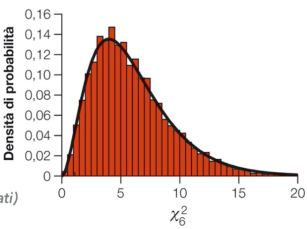
\includegraphics[width=0.6\textwidth]{fig8.2-1}
    \caption{\small{}}
    \end{figure}

Le caratteristiche essenziali della distribuzione teorica del $\chi^2$ (d'ora in avanti semplicemente "distribuzione $\chi^2$") sono state tabulate in tavole statistiche. %\TODO(UTILIZZO?)
\\
La distribuzione $\chi^2$ è in realtà una famiglia di distribuzioni, e quella particolare che serve per analizzare i dati sulle nascite è specificata dal numero di \textbf{gradi di libertà} (df, degrees of freedom):
\begin{equation}
df = (numero\ di\ categorie) -1 - (numero\ di\ parametri\ stimato\ in\ base\ ai\ dati)
\end{equation}
Nell'esempio corrente, l'ultimo termine dell'equazione è pari a zero (successivamente si capirà a cosa si riferisce). I dati sulle nascite hanno 7 categorie, una per giorno della settimana, quindi i gradi di libertà sono $7-1 = 6$, quindi il valore di $\chi^2$ calcolato in base ai dati osservati ($\chi^2 = 15.05$) deve essere confrontato con la distribuzione $\chi^2_6$.
\\
Tale distribuzione è rappresentata dalla curva nera nella figura \ref{fig8.2-1}

\subsection{Calcolo del P-value}
Per il test $\chi^2$ di bontà dell'adattamento, il P-value è la probabilità di ottenere un valore del $\chi^2$ maggiore del valore osservato, ovvero calcolato in base ai dati.
\\
Se i dati rispecchiassero esattamente quanto previsto dall'ipotesi nulla, $\chi^2$ sarebbe 0, mentre più è marcata la differenza dai valori attesi, maggiore è il valore di $\chi^2$, per cui per calcolare il P-value si usa solo la coda destra della distribuzione $\chi^2$.
\\
La distribuzione $\chi^2$ è una distribuzione di probabilità continua, quindi la probabilità è data dall'area della regione sottesa dalla curva. La probabilità di ottenere un valore del $\chi^2$ maggiore di un singolo valore specificato, necessario per calcolare il P-value, è uguale all'area sotto la curva a destra di tale valore fino all'infinito.
\\
Nell'esempio, la probabilità di ottenere un valore uguale o superiore a 15.05 è uguale all'area sottesa dalla curva $\chi^2_6$ oltre 15.05:
\clearpage
    \begin{figure}[h]\label{fig8.2-2}
    \centering
    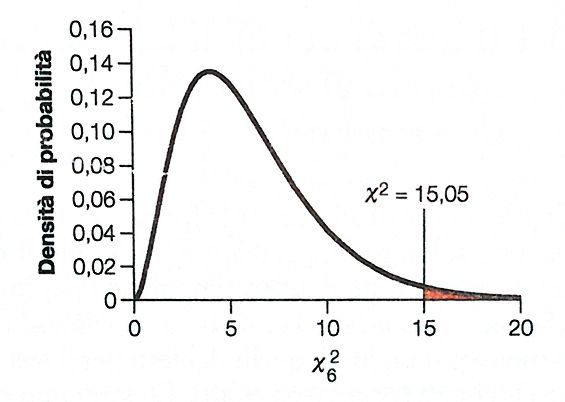
\includegraphics[width=0.6\textwidth]{fig8.2-2}
    \caption{\small{}}
    \end{figure}
Per calcolare l'area a destra del valore di $\chi^2$ calcolato a partire dai dati si hanno due opzioni:
\begin{itemize} \tightlist
    \item Utilizzare un programma statistico al computer.
    \\
    Il P-value che si ottiene in tale modo è $P = 0.0199$ che, al livello si sigificatività standard $\alpha = 0.05$ induce a rifiutare l'ipotesi nulla. I dati forniscono quindi evidenze del fatto che le nascite non sono distribuite casualmente nei giorni della settimana.
    \item Utilizzare dei valori critici.
    \\
    Un \textbf{valore critico} è il valore di una statistica test che identifica il confine di un'area specificata nella coda (o nelle code) della distribuzione campionaria sotto l'ipotesi nulla; ad esempio, con un $\alpha = 0.05$, il valore di $\chi^2$ per il quale l'area sottesa dalla curva alla sua destra è pari a 0.05 è detto "valore critico corrispondente ad $\alpha = 0.05$".
    \\
    I valori critici della distribuzione $\chi^2$ sono tabulati nella Tavola statistica A (\ref{tavA}).
    %Come usare la tabella: individuare la colonna corrispondente al livello di significatività desiderato ($\alpha&); individuare la riga corrispondente al numero di gradi di libertà ($df$) per la statistica test. Il numero nella casella corrispondente è il valore critico.
    \\
    Nell'esempio, il valore critico è pari a 12.59, quindi, sotto l'ipotesi nulla, la probabilità di ottenere un valore di $\chi^2$ altrettanto o più estremo di 12.59 è pari a 0.05:
    \begin{equation}
    Pr[\chi^2_6 \ge 15.05] = 0.05
    \end{equation}
    e si rifiuta quindi l'ipotesi nulla.
\end{itemize}

\subsection{Assunzioni del test \texorpdfstring{$\chi^2$}{Lg} di bontà dell'adattamento}

Il test $\chi^2$ di bontà dell'adattamento assume che gli individui nell'insieme dei dati siano un campione casuale estratto dall'intera popolazione, ovvero che ogni individuo sia stato scelto indipendentemente da tutti gli altrie che ogni individuo della popolazione ha avuto la stessa probabilità di essere incluso.
\\
La distribuzione campionaria della statistica $\chi^2$ segue una distribuzione $\chi^2$ solo approssimativamente, anche se l'approssimaizone è molto buona quando si seguono due regole:
\begin{itemize} \tightlist
    \item nessuna delle categorie deve avere una frequenza attesa minore di 1;
    \item non più del 20\% delle categorie deve avere frequenze attese minori di 5.
\end{itemize}
Queste restrizioni si riferiscono alle frequenze attese e non a quelle osservate; se tali condizioni non sono soddisfatte, il test diventa inaffidabile.
\\
Se una delle condizioni non è soddisfatta, si hanno due opzioni:
\begin{itemize} \tightlist
    \item raggruppare, se possibilie, alcune delle categorie con frequenze attese piccole, per ottenere meno categorie, che abiano però frequenze attese maggiori (si devono cambiare di conseguenza i gradi di libertà);
    \item trovare un alternativa al test del $\chi^2$ (es. simulaizoni al computer).
\end{itemize}

\subsection{Test del \texorpdfstring{$\chi^2$}{Lg} con due sole categorie}

Il test del $\chi^2$ funziona anche quando vi sono solo due categorie, per cui si può usare anche in sostituzione del test binomiale, purché siano soddisfatte le relative assunzioni. I calcoli sono più rapidi ma meno esatti di quelli di un test binomiale.

\begin{example}[contenuto genico del cromosoma X umano]
    Ad ora sappiamo che il cromosoma X dell'uomo contiene 781 dei 20290 geni trovati finora, e che il cromosoma X contiene circa il 5.2\% del DNA totale.
    \\
    Assumendo il modello proporzionale, ci si aspetterebbe che il 5.2\% dei geni fosse localizzato su tale cromosoma. È così?
    \\
    Definiamo le ipotesi:
    \begin{itemize} \tightlist
        \item $H_0$: la percentuale dei geni umani sul cromosoma X è 5.2\%;
        \item $H_A$: la percentuale dei geni umani sul cromosoma X non è 5.2\%
    \end{itemize}
    Il numero atteso di geni sul cromosoma X umano è $20290 x 0.052 = 1055$, quindi un numero molto maggiore rispetto a quello dei geni osservati (781).
    \\
    Si vuole stabilire qual è la probabilità di un risultato altrettanto o più estremo di quello osservato se fosse vera l'ipotesi nulla.
    \\
    Calcolare il P-value con il test binomiale sarebbe impegnativo, poiché il numero di prove (geni) è $n = 20290$ e la probabilità che un gene sia presente sul cromosoma X  è $p = 0.052$. Quindi, il valore di P si calcolerebbe come:
    \begin{equation}
    P =\ 2\ x\ Pr[X\le781]\ =\ 2\ x\ (Pr[X=0] + Pr[X=1] + Pr[X = 2] +\ ...\ + Pr[X = 781])
    \end{equation}
    Usando il test $\chi^2$, invece:
    \begin{equation}
    \chi^2 = \frac{(781-1055)^2}{1055}+\frac{(19509-19235)^2}{19235} = 75.1
    \end{equation}
    Questa statistica ha due categorie, e quindi un solo grado di libertà ($df = 2-1 = 1$).
    Dall'appendice %\ref{appvaloricritici}
    si vede che il valore critico per $\chi^2_1$ per un $\alpha=0.05$ è pari a 3.84 e, poiché il $\chi^2$ osservato, 75.1, è maggiore di 3.84, si può dire che $P\ <\ 0.05$ e rifiutare l'ipotesi nulla.
    \\
    In realtà, dal momento che il $\chi^2$ calcolato è maggiore anche del più grande valore critico tabulato per un $df[\chi^2_{1,(0.001)} = 10.83]$, si può dire che $P\ <\ 0.001$, e dunque che, nella specie umana, il numero di geni sul cromosoma X è significativamente minore di quello che ci si aspetterebbe in base alle dimensioni di tale cromosoma.
\end{example}
Dunque, nel caso di due sole categorie, il test binomiale è l'opzione migliore per $n$ piccoli e quando le frequenze attese sono troppo basse per soddisfare le assunzioni del test $\chi^2$; inoltre, tale test è preferibile anche per $n$ grandi quando si dispone di un computer, poiché fornisce un P-value esatto.

\section{Adattamento della distribuzione binomiale}

La distribuzione binomiale descrive la probabilità di ottenere $X$ successi in $n$ prove indipendenti.

\begin{example}[famiglie pianificate]
Ci si aspetta che il numero di maschi e di femmine nati in famiglie con 2 figli siano conformi ad una distribuzione binomiale, con $n =2$ e $p$ uguale alla probabilità di avere un maschio in ogni singola prova.
\\
È questo ciò che si osserva?
\\
Per le famiglie con 2 figli sono possibili 3 risultati: 0, 1 o 2 maschi; la tabella \ref{tabmaschi} riporta i dati raccolti per 2444 famiglie:
    \begin{table}[H]
        \centering
        \renewcommand\arraystretch{1.2}
        \begin{tabular}{c|c}
        \hline
        \textbf{Numero maschi} & \textbf{Numero osservato di famiglie} \\
        \hline
        0 & 530 \\
        1 & 1332 \\
        2 & 582 \\
        \hline
        \textbf{Totale} & 2444 \\
        \hline
        \end{tabular}
        \caption{}
        \label{tabmaschi}
    \end{table}\noindent
    L'adattamento della distribuzione binomiale ai dati si può verificare con il test del $\chi^2$.
    \\
Definiamo le ipotesi:
    \begin{itemize} \tightlist
    \item $H_0$: il numero di maschi nella famiglie con 2 figli ha una distribuzione binomiale;
    \item $H_A$: il numero di maschi nella famiglie con 2 figli non ha una distribuzione binomiale.
    \end{itemize}
    Si sta quindi verificando l'adattamento di una distribuzione ai dati osservati in più famiglie, non un'ipotesi sulla proporzione media di maschi.
    \\
    Quando si testa l'adattamento ad una distribuzione binomiale, si studiano i risultati ottenuti in più set di prove, confrontando un set di frequenze con i corrispondenti valori previsti dalla distribuzione. Tale procedura è diversa dall'impiego della distribuzione binomiale per verificare un'ipotesi nulla su una singola proporzione: in un test binomiale si ha un solo set di prove.
    \\
    In questo caso, l'ipotesi nulla non specifica $p$, la probabilità che un singolo figlio sia maschio, quindi si deve stimare $p$ in base ai dati prima di poter calcolare le frequenze attese.
    \\
    Nello studio ci sono 4888 figli; il numero totale di maschi è $(2 x 582) + 1332 = 2496$, perciò, la probabilità che un figlio sia maschio è:
    \begin{equation}
    \hat{p} = \frac{2496}{4888} = 0.5106
    \end{equation}
    Tale stima, assieme alla distribuzione binomiale con $n = 2$, si usano per calcolare le frequenze attese sott l'ipotesi nulla; ad esempio, la frazione attesa di famiglie con 2 figli che hanno 1 solo maschio è:
    \begin{equation}
    Pr[1\ maschio] = \binom{2}{1}\ (0.5106)^1\ (1-0.5106)^1 = 0.49977
    \end{equation}
    Quindi, la frequenza attesa di 2444 famiglie con 2 figli ed 1 solo maschio è:
    \begin{equation}
    Atteso\ (1\ maschio) = 2444 < 0.49977 = 1221.4
    \end{equation}
    Le frequenze attese per tutti i risultati possibili sono riportate in tabella \ref{tabmaschi2}:
    \begin{table}[H]
        \centering
        \renewcommand\arraystretch{1.2}
        \begin{tabular}{c|c|c}
        \hline
        \textbf{Numero maschi} & \textbf{Numero osservato di famiglie} & \textbf{Numero atteso di famiglie}\\
        \hline
        0 & 530 & 585.3\\
        1 & 1332 & 1221.4\\
        2 & 582 & 637.3\\
        \hline
        \textbf{Totale} & 2444 & 2444.0\\
        \hline
        \end{tabular}
        \caption{}
        \label{tabmaschi2}
    \end{table}\noindent
    E i valori attesi assieme ai dati osservati sono rappresentati nella Figura \ref{fig8.5-1}:
    \begin{figure}[H]\label{fig8.5-1}
    \centering
    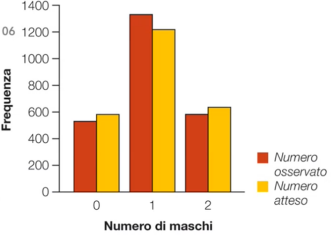
\includegraphics[width=0.6\textwidth]{fig8.5-1}
    \caption{\small{}}
    \end{figure}
    Nell'esempio corrente, le frequenze osservate non sono uguali a quelle attese; esiste infatti un eccesso di famiglie con 2 figli ed 1 solo figlio maschio, rispetto alle altre due tipologie.
    \\
    Si vuole stabilire se tale differenza sia attribuibile al caso o se sia motivo di rifiuto dell'ipotesi nulla.
    \\
    Si calcola il $\chi^2$:
    \begin{equation}
    \chi^2 = \frac{(530-585.3)^2}{585.3}+\frac{(1332-1221.4)^2}{1221.4}+\frac{(582-637.3)^2}{637.3}
    \end{equation}
    Per calcolare il numero di gradi di libertà si considera che si hanno 3 categorie; di norma, dunque, i gradi sarebber 2; tuttavia, in questo caso si è dovuto stimare un parametro a partire dai dati per calcolare le frequenze attese ($p$), quindi:
    \begin{equation}
    df = 3-1-1 = 1
    \end{equation}
    Il valore critico per la distribuzione $\chi^2_1$ con un grado di libertà ed $\alpha= 0.05$ è pari a 3.84. Poiché 20.04 è localizzato verso destra nella coda della distribuzione rispetto a 3.84, $P < 0.05$, quindi si rifiuta l'ipotesi nulla.
    \\
    Dunque, la distribuzione di frequenza del numero di maschi e femmine nelle famiglie con 2 figli non è governata dalla distribuzione binomiale, quindi in questi dati una delle assunzioni della distribuzione binomiale deve essere rifiutata: la probabilità di avere un maschio varia da famiglia a famiglia e/o gli individui nella stessa famiglia non sono indipendenti l'uno dall'altro.
    \\
    Una probabile spiegazione è che le famiglie con 2 senza maschi o senza femmine siano insoddisfatte e decidano di avere un terzo figlio, rimuovendosi dall'insieme di famiglie con 2 soli figli.
\end{example}

\subsection{Test binomiale per \textit{n} grandi}\footnote{da spiegazione del prof. Massolo, fine della lezione 20211115}
\\
Una distribuzione di casi con $p$ vicini allo 0.5 ed $n$ vicini al 40 tende ad assumere la forma di una curva normale; quindi quando si hanno distribuzioni più o meno binomiali, invece di usare la distribuzione binomiale si può, usando i parametri:
\begin{itemize} \tightlist
    \item $\mu = np$;
    \item $\sigma = \sqrt{np\ (1-p)}$.
\end{itemize}
stimare il valore $z$:
\begin{equation}
z = \frac{x_i-\mu}{\sigma}
\end{equation}
Se il valore di $z$ che si ottiene è superiore ad 1.96, si può rifiutare l'ipotesi nulla.

\section{Distribuzione di Poisson}

La \textbf{distribuzione di Poisson} indica la probabilità di ottenere $X$ successi in un certo intervallo di tempo o in una certa porzione di spazio, quando ogni successo si verifica indipendentemente e con uguale probabilità in ogni punto del tempo e dello spazio.

\begin{example}[Esempio: ragni dopo l'eruzione]
Dopo un'eruzione, i ragni sono i primi animali a ricolonizzare il territorio, trasportati dai venti.
\\
Come sarebbe la distribuzione dei ragni, se l'atterraggio fosse casuale nello spazio?
\\
Si fanno due assunzioni:
\begin{itemize} \tightlist
    \item la probabilità che un ragno atterri in un dato punto è la stessa in ogni punto del territorio considerato;
    \item il fatto che un ragno atterri in un dato punto è indipendente dagli atterraggi in ogni altro punto (quindi i ragni non si raggruppano né si respingono tra loro).
\end{itemize}
Per contare i ragni, si suddivide il territorio d'interesse in tante porzioni di uguale dimensione, grandi a sufficienza da contenere molti potenziali siti di atterraggio.
\\
Se entrambi gli assunti sono soddisfatti, la distribuzione di frequenza del numero di ragni che atterrano nelle porzioni di suolo seguirà una distribuzione di Poisson.
\end{example}
È lecito aspettarsi una distribuzione di Poisson per certi conteggi in biologia (es. numero di mutazioni in ogni individuo di una popolazione, numero di salmoni catturati inun giorno da un predatore, numero di semi germinanti per ogni pianta). Un fenomeno diventa interessante quando non segue il modello semplice di partenza, perché in tal caso si scopre che alcune delle assunzioni fatte sono false, il che suggerisce l'esistenza di processi particolari (es. alcuni individui possono essere effettivamente più inclini alle mutazioni di altri, alcuni predatori più bravi nella cattura di altri, alcune piante produrre semi di maggior successo).
\\
Dunque, mentre la distribuzione di poisson prevede una distribuzione \textbf{casuale} dei successi, le alternative ad essa prevedono distribuzioni non casuali nel tempo e nello spazio; i successi, ad esempio, possono essere:
\begin{itemize} \tightlist
    \item \textbf{raggruppati} (o agglomerati), ovvero possono avvenire più vicini l'uno a l'altro di quanto ci si aspetterebbe per effetto del caso, come potrebbe succedere, ad esempio, quando la presenza di un successo aumenta la probabilità che si verifichino altri successi in prossimità (es. epidemie di malattie contagiiose);
    \item \textbf{dispersi}, ovvero possono avere una distribuzione più uniforme di quella attesa per effetto del caso, come può accedere quando la presenza di un successo diminuisce la probabilità che ci siano altri successi in prossimità (es. distribuzione degli animali territoriali).
\end{itemize}
    \begin{figure}[h]\label{fig8.6-1}
    \centering
    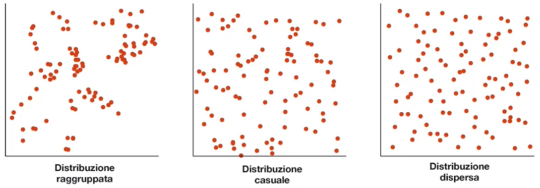
\includegraphics[width=0.6\textwidth]{fig8.6-1}
    \caption{\small{}}
    \end{figure}
Le deviazioni da pattern casuali possono quindi evidenziare processi biologici interessanti.
\\
La formula matematica della distribuzione di Poisson descrive la probabilità che si verifichino $X$ successi in qualsiasi intervallo di tempo o porzioni di spazio:
\begin{equation}
Pr[X\ successi] = \frac{e^{-\mu}\mu^X}{X!}
\end{equation}
In cui:
\begin{itemize} \tightlist
    \item \textbf{$\mu$} è il numero medio di successi indipendenti nello spazio e nel tempo, espressi come conteggio riferito all'unità di tempo o di spazio;
    \item \textbf{$e$} è la base dei logaritmi naturali (2.718...).
\end{itemize}
Se si immagina di dividere un intervallo di tempo in moltissimi intervalli più brevi (stesso ragionamento si potrebbe applicare alla dimensione spaziale), la probabilità che ha un evento di verificarsi in ognuno di essi sarà prossima a zero, quindi per ciascuno di tali intervalli potranno esserci due possibili situazioni:
\begin{itemize} \tightlist
    \item l'evento di verifica una volta, con probabilità molto piccola;
    \item l'evento non si verifica, con probabilità molto grande.
\end{itemize}
Non potranno quindi esistere intervalli in cui un evento si verifica più di una volta. In questo modo, si riconduce la distribuzione di Poisson del numero di eventi che possono avvenire in un certo intervallo di tempo (o in una certa area) ad una distribuzione binomiale; ci sono infatti due soli eventi possibili nella singola prova, successo o insuccesso, ma in questo caso il numero di prove (numero di potenziali successi, es. potenziali siti di atterraggio dei ragni in ogni plot) è enorme, e la probabilità di successo della singola prova (un ragno che atterra in un punto specifico) tende a zero. Si può in effetti dimostrare che la distribuzione di Poisson si può ottenere come limite della distribuzione binomiale per $p$ che tende a zero ed $n$ che tende ad infinito. Il prodotto $np$ corrisponde al numero medio di eventi per intervallo (o area), ovvero al parametro $\mu$ della distribuzione di Poisson.

\subsection{Verifica della casualità con la distribuzione di Poisson}
In biologia, la distribuzione di Poisson si impiega principalmente per formulare ipotesi nulle e verificare se i successi siano distribuiti casualmente nel tempo e nello spazio.
\\
Di solito nnon si conosce il tasso esatto con cui si verificano i successi, quindi per poter fare previsioni sulla probabilità di diversi risultati in base ad una distribuzione di Poisson si deve prima stimare il tasso di successi in base ai dati.
\begin{example}[estinzioni di massa\label{esestinzioni}]
La tabella \ref{tabestinzioni} riporta il numero di estinzioni di famiglie di invertebrati marini registrate in 76 intervalli di tempo di durata simile, stimate sulla base di testimonianze fossili.
\begin{table}[H]
        \centering
        \renewcommand\arraystretch{1.2}
        \begin{tabular}{c|c}
        \hline
        \textbf{Numero estinzioni ($X$)} & \textbf{Frequenza}\\
        \hline
        0 & 0 \\
        1 & 13 \\
        2 & 15 \\
        3 & 16 \\
        4 & 7 \\
        5 & 10 \\
        6 & 4 \\
        7 & 2 \\
        8 & 1 \\
        9 & 2 \\
        10 & 1 \\
        11 & 1 \\
        12 & 0 \\
        13 & 0 \\
        14 & 1 \\
        15 & 0 \\
        16 & 2 \\
        17 & 0 \\
        18 & 0 \\
        19 & 0 \\
        20 & 1 \\
        >20 & 0 \\
        \hline
        \textbf{Totale} & 76 \\
        \hline
        \end{tabular}
        \caption{}
        \label{tabestinzioni}
\end{table}\noindent
Le estinzioni si verificano casualmente, o ci sono periodi in cui i tassi di estinzione sono insolitamente elevati (estinzioni di massa)?
\\
Se l'estinzione delle famiglie fosse casuale nel tempo, il numero di estinzioni in ogni intervallo dovrebbe seguire una distribuzione di Poisson; le alternative sono (1) che le estinzioni siano raggruppate nel tempo e che avvengano dunque delle estinzioni di massa, oppure (2) che le estinzioni avvengano più uniformemente nel tempo di quanto ci si aspetterebbe casualmente.
\\
Per capire quale dei tre sia il caso, si confronta la distribuzione di frequenza delle estinzioni delle famiglie con quella prevista da una distribuzione di Poisson usando il test del $\chi^2$.
\\
Le ipotesi sono:
\begin{itemize} \tightlist
    \item $H_0$: il numero di estinzioni per ogni intervallo di tempo ha una distribuzione di Poisson;
    \item $H_A$: il numero di estinzioni per ogni intervallo di tempo non ha una distribuzione di Poisson.
\end{itemize}
Prima di effettuare il test, si calcola $\mu$, che in questo caso corrisponde al numero medio di di estinzioni per ogni intervallo di tempo, attraverso la media campionaria:
\begin{equation}
\overline{X} = \frac{(0x0)+(13x1)+(15x2)+...}{76} = 4.21
\end{equation}
Tale media campionaria è usata al posto di $\mu$ nella formula per la distribuzione di Poisson per generare le frequenze attese.
\\
L'istogramma in figura \ref{fig8.6-2} rappresenta la distribuzione di frequenza osservata del numero di estinzioni per intervallo di tempo, mentre il diagramma a segmenti congiunge le frequenze previste dell'ipotesi nulla (distribuzione di Poisson).
    \begin{figure}[H]\label{fig8.6-2}
    \centering
    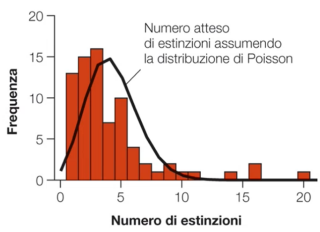
\includegraphics[width=0.6\textwidth]{fig8.6-2}
    \caption{\small{}}
    \end{figure}
Si nota una discrepanza: rispetto alla distribuzione di Poisson, le testimonianze fossili presentano troppi intervalli di tempo con moltissime estinzioni e troppi intervalli di tempo con pochissime estinzioni.
\\
Il divario che si osserva è maggiore di quello che ci si aspetterebbe per effetto del caso? Per stabilirlo si usa il test del $\chi^2$.
\\
Per calcolare le frequenze attese nelle diverse categorie di estinzioni, tranne l'ultima, si applica la formula della distribuzione di Poisson per il calcolo delle probabilità attese, che poi vanno moltiplicate per il numero totale di intervalli di tempo (76); ad esempio, la probabilità attesa e poi la frequenza attesa degli intervalli di tempo con tre estinzioni sono:
\begin{equation}
Pr[3\ estinzioni] = \frac{e^{-\mu}\mu^3}{3!} = \frac{e^{-4.21}4.21^3}{3!} = 0.1846
\end{equation}
\begin{equation}
Frequenza\ attesa[3\ estinzioni] = 76 x 0.1846 = 14.03
\end{equation}
Nell'ultima categoria si raggruppano tutte le $X \ge 10$ estinzioni perché la frequenza attesa dei numeri più grandi diventa molto piccola; per calcolarla, si sottrae la somma di tutti i valori attesi precedenti da 76, ovvero il numero totale di intervalli di tempo.
\\
Le frequenze attese non soddisfano gli assunti del test del $\chi^2$, dato che una di esse è minore di 1 e più del 20\% sono minori di 5; in questi casi, si possono raggruppare le categorie e tentare nuovamente, ad esempio, si possono riunire in un'unica categoria $X = 0$ ed $X = 1$, ed in un'altre tutte le categorie con $X \ge 8$, dato che le categorie raggruppate sono simili. I dati che si ottengono hanno 8 categorie, riportate nella tabella \ref{tabestinzioni2}:
\begin{table}[H]
        \centering
        \renewcommand\arraystretch{1.2}
        \begin{tabular}{c|c|c}
        \hline
        \textbf{Numero estinzioni ($X$)} & \textbf{\makecell{Frequenza osservata\\di intervalli di tempo}} & \textbf{\makecell{Frequenza attesa\\di intervalli di tempo}}\\
        \hline
        0 o 1 & 13 & 5.88 \\
        2 & 15 & 10.00\\
        3 & 16 & 14.03\\
        4 & 7 & 14.77\\
        5 & 10 & 12.44\\
        6 & 4 & 8.72\\
        7 & 2 & 5.24 \\
        >8 & 9&4.91 \\
        \hline
        \textbf{Totale} & 76 & 76\\
        \hline
        \end{tabular}
        \caption{}
        \label{tabestinzioni2}
\end{table}\noindent
Usando la formula standard per la statistica $\chi^2$ si ottiene:
\begin{equation}
\chi^2 = \frac{(13-5,88)^2}{5.88}+\frac{(15-10)^2}{10}+\frac{(16-14.03)^2}{14.03}+... = 23.93
\end{equation}
Per il test si hanno 6 gradi di libertà, dato che si deve tener conto del parametro $\mu$ che è stato calcolato a partire dai dati, e quindi $df = 8-1-1=6$.
\\
Il valore critico per la $\chi^2_{6,(0.05)}$ è 12.59. Dato che la statistica $\chi^2$ è interna alla coda della distribuzione rispetto al valore critico, il P-value è minore di 0.05 (ed anche di 0.001, dato che 23.93 è anche maggiore di 22.46, che è il valore critico per $\alpha = 0.001$). Si rifiuta quindi l'ipotesi nulla e si conclude che le estinzioni d'interesse non si adattano ad una distribuzione di Poisson.
\end{example}

%%%%%LIBRO FINE CAPITOLO 8, CONTROINTUITIVO E OPPOSTO A QUELLO CHE DICE IL PROF, NELLA PROSSIMA SOTTOSEZIONE
% \subsection{Confronto tra media e varianza per descrivere il discostamento dalla distribuzione di Poisson}
% Una proprietà della distribuzione di Poisson è che la varianza del numero di successi per ogni intervallo di tempo (il quadrato della deviazione standard) è uguale alla media ($\mu$). Se la varianza è maggiore della media, allora la distribuzione è raggruppata, mentre, se è minore, la distribuzione è dispersa.
% \\
% Nell'esempio \ref{esestinzioni}, la media campionaria di estinzioni è 4.21. La varianza campionaria del numero di estinzioni è:
% \begin{equation}
% s^2 = \frac{(0-4.21)^2(0)+(1-4.21)^2(13)+(2-4.21)^2(15)+...}{76-1} = 13.72
% \end{equation}
% Quindi, dato che la varianza è molto maggiore della media, la distribuzione degli eventi di estinzione nel tempo è molto raggruppata.

\subsection{Indice di dispersione per descrivere il discostamento dalla distribuzione di Poisson}\footnote{da spiegazione del prof. Massolo, lezione 20211117 (1:17:00)}
\\
L'\textbf{indice di dispersione} ($D$, o variance to mean ratio, $VMR$) esprime il rapporto tra varianza e media:
\begin{equation}
VMR = \frac{\sigma^2}{\mu}
\end{equation}
Nella distribuzione di Poisson, varianza e media sono uguali, quindi il $VMR$ è pari ad 1.
\\
Se i due valori differiscono si possono avere due casi:
\begin{itemize} \tightlist
    \item $VMR > 1$ ($\sigma^2 > \mu$): la distribuzione è dispersa (come nella distribuzione binomiale negativa);
    \item $VMR < 1$ ($\sigma^2 < \mu$): la distribuzione è sotto-dispersa, quindi raggruppata (nella distribuzione è binomiale $0 < VMR < 1$).
\end{itemize}

\chapter{Analisi dell'associazione tra variabili categoriche (B5)}\footnote{Capitolo 9, Whitlock and Schluter, Analisi statistica dei dati biologici (2010)}

\section{Associazione tra due variabili categoriche}
L'esistenza di un'associazione tra due variabili categoriche implica che esse non siano indipendenti.
\\
Se le due variabili fossero indipendenti, la probabilità attesa di osservare una combinazione qualsiasi delle categorie appartenenti alle due variabili (es. categoria A per la variabile 1 e categoria C per la variabile 2) sarebbe:
\begin{equation}
Pr[A\ e C] = Pr[A] Pr[C]
\end{equation}
Se invece non sono indipendenti, la probabilità di ottenere la combinazione è diversa dal semplice prodotto.
\begin{example}[naufragio del Titanic\label{estitanic}]
    Durante in naufragio del Titanic, sono morte meno donne che uomini, anche tenendo conto delle abbondanze relative delle due categorie.
    \\
    Per stabilire se la differenza osservata può essere attribuibile al caso o se ci sia stata un'associazione tra sesso e mortalità si può ricorrere al test del $\chi^2$, dal momento che si vogliono confrontare frequenze assolute.
    \\
    Nel caso dell'esempio corrente, sesso e mortalità non sono indipendenti.
    \\
    I dati sono riportati nella tabella \ref{tabtitanic}, mentre i mosaic plots \ref{fig9.1-1} mostrano la relazione tra sesso e mortalità osservata (a sinistra) ed attesa nel caso di variabili indipendenti (destra).
\begin{table}[H]
        \centering
        \renewcommand\arraystretch{1.2}
        \begin{tabular}{c|c|c|c}
        \hline
         & \textbf{Deceduti (D)} & \textbf{Sopravvissuti (S)} & \\
        \hline
        \textbf{M} & 1364 & 367 & 1731 \\
        \hline
        \textbf{F} & 126 & 344 & 470\\
        \hline
         & 1490 & 711 & \textbf{2201}\\
        \hline
        \end{tabular}
        \caption{}
        \label{tabtitanic}
\end{table}\noindent
    \begin{figure}[H]\label{fig9.1-1}
    \centering
    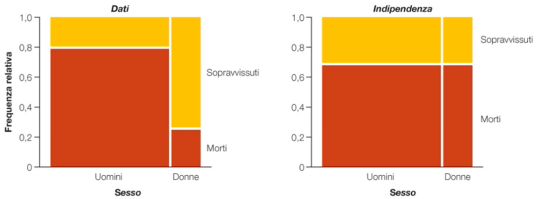
\includegraphics[width=0.6\textwidth]{fig9.1-1}
    \caption{\small{}}
    \end{figure}
\end{example}

\section{Stima dell'associazione in tabelle \texorpdfstring{$2 x 2$}{Lg}: odds ratio}

L'\textbf{odds ratio} misura l'entità dell'associazione tra due variabili categoriche quando ciascuna di esse ha solo due categorie; una delle due variabili è la \textbf{variabile risposta}, che ha le due categorie "successo" ed "insuccesso", mentre l'altra è la \textbf{variabile esplicativa}, le cui due categorie identificano i due gruppi all'interno dei quali le probabilità di successo vengono calcolate e confrontate.
\\
Nell'esempio \ref{estitanic}, la categoria variabile è "morte", con categorie "successo" ed "insuccesso", mentre la variabile esplicativa è "sesso", che può assumere i valori "maschio" e "femmina".
\\
L'odds ratio confronta la proporzione di successi ed insuccessi tra i due gruppi.
\\
L'\textbf{odds} ($O$) di un successo è dato da:
\begin{equation}
O = \frac{p}{1-p}
\end{equation}
In cui $p$ è la probabilità di successo, e $1-p$ è la probabilità di insuccesso.
\\
Se $O = 1$, si verifica un successo per ogni insuccesso.
\\
Nell'esempio \ref{estitanic}, la probabilità di morire se si è maschi o femmine è data da:
\begin{equation}
O_M = \frac{p_{D|M}}{1-p_{D|M}}
\end{equation}
\begin{equation}
O_F = \frac{p_{D|F}}{1-p_{D|F}}
\end{equation}
In cui $p_{D|M}$ e $p_{D|F}$ corrispondono al rapporto tra deceduti maschi o femmine ed il totale di maschi o femmine.
\\
L'odds ratio è il rapporto tra i due odds (conviene mettere al denominatore la categoria della variabile esplicativa che si pensa possa avere più successo):
\begin{equation}
OR = \frac{\frac{p_{D|M}}{1-p_{D|M}}}{\frac{p_{D|F}}{1-p_{D|F}}}
\end{equation}
Le situazioni possono essere due:
\begin{itemize} \tightlist
    \item odds ratio = 1 (quindi odds dei maschi ed odds delle femmine sono uguali), quindi tra le due variabili considerate non c'è nessuna associazione;
    \item odds ratio $\neq$ 1, quindi tra le due variabili considerate c'è un'associazione.
\end{itemize}
Ovviamente, la differenza da 1 dev'essere statisticamente significativa.

\subsection{Errore associato all'odds ratio}
Quando l'odds ratio si calcola a partire da proporzioni osservate di successi in base ad un campione, sia le proporzioni che l'odds ratio sono stime (e dunque si indicano come $\hat{p}$ e $\hat{OR}$). In tali casi, alla stima dell'odds ratio va accompagnata anche una stima dell'errore ad esso associato, e questo si fa calcolando l'\textbf{intervallo di confidenza dell'odds ratio}.
\\
Per ottenere l'intervallo di confidenza dell'odds ratio è necessario calcolare il logaritmo naturale dell'odds ratio ($ln(\hat{OR})$), poiché l'odds ratio ha una distribuzione non normale.
\\
L'errore standard del logaritmo naturale dell'odds ratio si calcola come:
\begin{equation}
ES[ln(\hat{OR})] = \sqrt{\frac{1}{a}+\frac{1}{b}+\frac{1}{c}+\frac{1}{d}}
\end{equation}
In cui $a$, $b$, $c$ e $d$ si riferiscono alle frequenze osservate nelle celle della tabella di ocntingenza (nell'esempio \ref{estitanic}, i quattro valori principali nella tabella \ref{tabtitanic}).
\\
L'intervallo di confidenza viene quindi calcolato come:
\begin{align*}
    ln(\hat{OR})\ -\ Z\ ES[ln(\hat{OR})]\ <\ ln(\hat{OR})\ <\ ln(\hat{OR})\ +\ Z\ ES[ln(\hat{OR})]
    \\ \\
    \Rightarrow e^{ln(\hat{OR})\ -\ Z\ ES[ln(\hat{OR})]}\ <\ \hat{OR}\ <\ e^{ln(\hat{OR})\ +\ Z\ ES[ln(\hat{OR})]}
\end{align*}
In cui il valore di $Z$ dipende dal tipo di intervallo di confidenza che si vuole calcolare (es. per un intervallo di confidenza al 95\% $Z = 1.96$).
\\


\begin{example}[Esempio: aspirina]
29876 donne sono state sottoposte casualmente a due trattamenti diversi: 19934 hanno ricevuto 100 mg di aspirina a giorni alterni, 19942 hanno ricevuto un placebo.
\\
Tali donne, ignare riguardo il tipo di trattamento ricevuto, sono state monitorate per 10 anni, durante i quali 1438 che ricevevano aspirina e 1427 che ricevevano il placebo hanno avuto una diagnosi di cancro invasivo.
\\
La tabella \ref{tabaspirina} riporta i dati, che sono rappresentati nel mosaic plot nella Figura \ref{fig9.2-1}.
\begin{table}[H]
        \centering
        \renewcommand\arraystretch{1.2}
        \begin{tabular}{c|c|c}
        \hline
         & \textbf{Aspirina (A)} & \textbf{Placebo (P)}\\
        \hline
        \textbf{Cancro (C)} & a = 1438 & b = 1427 \\
        \hline
        \textbf{No cancro (N)} & c = 18496 & d = 18515\\
        \hline
        \end{tabular}
        \caption{}
        \label{tabaspirina}
\end{table}\noindent
    \begin{figure}[H]\label{fig9.2-1}
    \centering
    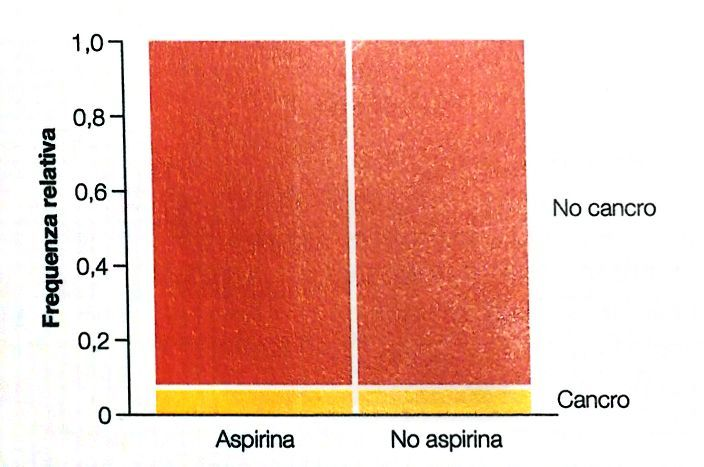
\includegraphics[width=0.6\textwidth]{fig9.2-1.png}
    \caption{\small{}}
    \end{figure}
    Il rischio di sviluppare cancro invasivo nelle donne è più elevato nelle pazienti che ricevono aspirina?
    \\
    RISOLVI QUESITO!
\end{example}

\begin{example}[covid-19\label{escovid2}]
LEZIONE 20211124
\end{example}

\section{Test del \texorpdfstring{$\chi^2$}{Lg} per stabilire la significatività dell'associazione tra due variabili categoriche}

Il test del $\chi^2$ è il test statistico più usato per verificare lì'associazione tra due variabili categoriche; tale test verifica la bontà di adattamento ai dati osservati di un modello nullo che assume l'indipendenza delle variabili.

\begin{example}[parassitosi e predazione\label{esparassitosi}]
Un trematode parassitizza un pesce, presumibilmente modificandone il comportamento ed inducendolo a nuotare a profondità minori, il che rende il pesce più vulnerabile alla predazione da parte di un uccello, che è un altro ospite del parassita.
\\
In una vasca all'aperto vengono posti tre diversi gruppi di pesci: non infestati, lievemente infestati e fortemente infestati; nella tabella \ref{tabparassitosi} è riportato il numero di pesci predati dagli uccelli a seconda del loro livello di infestazione:
\begin{table}[H]
        \centering
        \renewcommand\arraystretch{1.2}
        \begin{tabular}{c|c|c|c|c}
        \hline
         & \textbf{\makecell{Non\\infestati}} & \textbf{\makecell{Lievemente\\infestati}} & \textbf{\makecell{Fortemente\\infestati}} & \textbf{\makecell{Totali\\righe}}\\
        \hline
        \textbf{Predati} & 1 & 10 & 37 & 48\\
        \hline
        \textbf{Non predati} & 49 & 35 & 9 & 93\\
        \hline
        \textbf{Totali colonne} & 50 & 45 & 46 & 141\\
        \hline
        \end{tabular}
        \caption{}
        \label{tabparassitosi}
\end{table}\noindent
I dati sono rappresentati nel mosaic plot \ref{fig9.3-1}:
    \begin{figure}[H]\label{fig9.3-1}
    \centering
    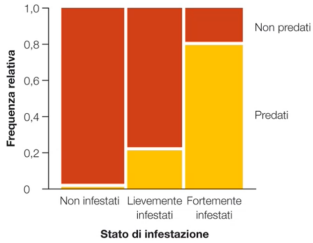
\includegraphics[width=0.6\textwidth]{fig9.3-1}
    \caption{\small{}}
    \end{figure}
Dai dati ottenuti risulta che solo il 2\% dei pesci non infestati viene predato, mentre il 22\% e l'80\% dei pesci lievemente e fortemente infestati viene predato.
\\
Si vuole verificare se la probabilità che i pesci vengano predati dipenda dal loro stato di infestazione parassitaria.
\\
Le ipotesi sono:
\begin{itemize} \tightlist
    \item $H_0$: parassitosi ed essere/non essere predati sono indipendenti;
    \item $H_A$: parassitosi ed essere/non essere predati non sono indipendenti.
\end{itemize}
Per effettuare il test del $\chi^2$ sulla tabella di contingenza si devono calcolare le frequenze attese per ciascuna cella nella tabella \ref{tabparassitosi}, assumendo che sia vera l'ipotesi nulla di indipendenza.

Seconod la regola del prodotto (\ref{secprodottodiprobabilità}), se due eventi sono indipendenti, la probabilità che si verifichino entrambi è pari alla probabilità che si verifichi un evento per la probabilità che si verifichi l'altro; tale regola può essere impiegata per calcolare le proporzioni attese di pesci in ciascuna categoria, e poi le frequenze attese sotto l'ipotesi nulla.
\\
Dunque, se l'infestazione e la predazione sono indipendenti, la probabilità che un pesce non infestato venga predato è:
\begin{equation}\label{for10.7}
    Pr[non\ infestato\ e\ predato] = Pr[non\ infestato]\ Pr[predato] 
\end{equation}
Per calcolare la frequenza attesa di pesci non infestati e predati si deve prima stimare la probabilità che un pesce sia non infestato e la probabilità che un pesce venga predato, valori che si possono stimare in base ai dati della tabella \ref{tabparassitosi}; dunque, la probabilità stimata che un pesce non sia infestato è data dal numero totale di pesci non infestati nel campione (50), diviso il numero totale di pesci (141), e quindi è pari a 0.3546.
\\
Stesso ragionamento vale per la probabilità stimata di essere predati, che quindi risulta essere 0.3404.
\\
Perciò, assumendo vera lìipotesi nulla di indipendenza, la probabilità stimata che un pesce sia non infestato e predato è pari a 0.1207, calcolata con la formula \ref{for10.7}.
Dunque, la frequenza attesa di pesci non infestati e predati sotto l'ipotesi nulla è data da tale probabilità (0.1207), moltiplicata per il numero totale di individui dell'insieme di dati (141), ed è quindi pari a 17.
\\
Ripetendo tale procedura per tutte le altre celle della tabella \ref{tabparassitosi} si ottengono e frequenze attese per tutte le possibili combinazioni di casi, riportate nella tabella \ref{tabparassitosi2}:
\begin{table}[H]
    \centering
    \renewcommand\arraystretch{1.2}
    \begin{tabular}{c|c|c|c|c}
    \hline
     & \textbf{\makecell{Non\\infestati}} & \textbf{\makecell{Lievemente\\infestati}} & \textbf{\makecell{Fortemente\\infestati}} & \textbf{\makecell{Totali\\righe}}\\
    \hline
    \textbf{Predati} & 17.0 & 15.3 & 15.7 & 48\\
    \hline
    \textbf{Non predati} & 33.0 & 29.7 & 30.3 & 93\\
    \hline
    \textbf{Totali colonne} & 50 & 45 & 46 & 141\\
    \hline
    \end{tabular}
    \caption{\small{Frequenze attese di pesci predati e non, in base allo stato di infestazione.}}
    \label{tabparassitosi2}
\end{table}\noindent
I totali di righe e colonne ottenuti sono uguali ai corrispondenti osservati, dal momento che sono state usate le proporzioni relative ai dati per calcolare le frequenze attese.

\subsection{Calcolo del \texorpdfstring{$\chi^2$}{Lg}}
Per verificare se le discrepanze tra i valori osservati e quelli attesi siano maggiori di quelle che ci si aspetterebbe per effetto del caso, si calcola il $\chi^2$.
\\
Indicando con "c" il numero di colonne e con "r" il numero di righe:
\begin{equation}
    \chi^2 = \sum^c_1 \sum^r_1 \frac{[osservato(colonna,\ riga)- atteso(colonna,\ riga)]^2}{atteso(colonna,\ riga)}
\end{equation}
Inserendo i dati:
\begin{equation}
    \chi^2 = \frac{(1-17)^2}{17}+\frac{(49-33)^2}{33}+\frac{(10-15.3)^2}{15.3}+\frac{(35-29.7)^2}{29.7}+\frac{(37-15.7)^2}{15.7}+\frac{(9-30.3)^2}{30.3} = 69.5
\end{equation}
La distribuzione del $\chi^2$ sotto l'ipotesi nulla è approssimata dalla distribuzione teorica del $\chi^2$. Per calcolare i gradi di libertà per la distribuzione del $\chi^2$ di interesse, si contano il numero di righe e di colonne nella tabella; il numero di gradi di libertà è dato da:
\begin{equation}
    df = (r-1)(c-1)
\end{equation}
Nell'esempio corrente, dunque, i gradi di libertà sono (2-1)(3-1) = 2.

\subsection{P-value}

Il valore critico per la distribuzione $\chi^2$ con $df = 2$ ed $\alpha = 0.05$ è pari a 5.99. Il valore osservato (69.5) si colloca verso l'esterno nella coda della distribuzione, essendo molto maggiore del valore critico; si rifiuta quindi l'ipotesi nulla: lo stato di infezione dei pesci influenza la probabilità che questi vengano predati.
\end{example}
Esiste anche una formula rapida per il calcolo delle frequenze attese (valore atteso nella cella di una tabella, corrispondente ad una certa riga e ad una certa colonna):
\begin{equation}
    atteso[riga\ i,\ colonna\ j] = \frac{(totale\ riga\ i)(totale\ colonna\ i)}{totale\ generale}
\end{equation}
Si può calcolare l'ultima cella in una riga o in una colonna anche per sottrazione, perché la somma delle frequenze attese per una data riga o colonna è uguale alla somma dei valori osservati.
\\
In una tabella di contingenza, il numero di celle in cui le frequenze non possono essere calcolate per differenza a partire dai totali di riga o colonna corrisponde anche ai gradi di libertà della distribuzione $\chi^2$ che dovrà essere utilizzata nel test; infatti, i gradi di libertà in un test del $\chi^2$ possono essere anche interpretati come il numero di categorie indipendenti, ovvero il numero di categorie sufficiente a calcolare, noti i totali di riga e colonna, tutti i valori nelle altre celle.
\\
\\
Il test del $\chi^2$ che si usa per l'analisi delle tabelle di contingenza è un'applicazione particolare del più generale test di bontà dell'adattamento; in questo caso, il modello probabilistico il cui possibile adattamento ai dati osservati viene verificato con il test è il modello che assume l'indipendenza delle variabili.

\subsection{Assunzioni del test \texorpdfstring{$\chi^2$}{Lg} per l'analisi delle tabelle di contingenza}
Le assunzioni del test del $\chi^2$ per l'analisi delle tabelle di contingenza sono le stesse del test del $\chi^2$ di bontà dell'adattamento.
\\
Se tali assunzioni non sono rispettate, sono disponibili almeno tre soluzioni:
\begin{itemize} \tightlist
    \item se la tabella è più grande di una $2x2$, allora due o più categorie nelle righe (o nelle colonne) possono essere combinate per ottenere frequenze attese maggiori; in tal caso si deve comunque evitare di ottenere categorie prive di significato;
    \item se la tabella è una $2x2$, si può impiegare il \textbf{test esatto di Fisher} (\ref{secfisher});
    \item si utilizza un test di randomizzazione. %TODO \ref{sec}
\end{itemize}

\section{Test esatto di Fisher}\label{secfisher}\footnote{non integrato con il libro, che ne parla a pagina 132.}
Il \textbf{test esatto di Fisher} si applica solo alle tabelle $2x2$ (teoricamente anche di dimensioni maggiori, ma molto complesso).
\begin{equation}
    p = \frac{}{}
\end{equation}
\begin{example}[cancro]\label{escancro}
    Si hanno 15 casi
    \begin{table}[H]
        \centering
        \renewcommand\arraystretch{1.2}
        \begin{tabular}{c|c|c|c|c}
        \hline
         & \textbf{Trattamento} & \textbf{No trattamento}\\
        \hline
        \textbf{Cancro} & a = 2 & b = 4 & \textbf{6} & 720 \\
        \hline
        \textbf{No cancro} & c = 8 & d = 1 & \textbf{9} & 362880\\
        \hline
        & \textbf{10} & \textbf{5} & \textbf{15} & \\
        \hline
        & 362880 & 120 &  & \\
        \hline
        \end{tabular}
        \caption{}
        \label{tabcancro}
    \end{table}\noindent
    Le frequenze attese corrispondenti sono riportate nella tabella \ref{tabcancro2}(es. calcolo per cella "a": (6*10)/15):
    \begin{table}[H]
        \centering
        \renewcommand\arraystretch{1.2}
        \begin{tabular}{c|c|c}
        \hline
        & \textbf{Trattamento} & \textbf{No trattamento}\\
        \hline
        \textbf{Cancro} & 4 & 2\\
        \hline
        \textbf{No cancro} & 6 & 3\\
        \hline
        \end{tabular}
        \caption{\small{Frequenze attese }}
        \label{tabcancro2}
    \end{table}\noindent
    Se non ci fossero violazioni delle assunzioni del test del $\chi^2$ si potrebbe proseguire con tale statistica; tuttavia, nell'esempio corrente, tre delle quattro celle hanno dei valori attesi inferiori a 5. Si usa dunque il test di Fisher.
    \\
    La formulazione del test di Fisher con quattro celle è:
    \begin{equation}
        p = \frac{(a+b)!(c+d)!(a+c)!(b+d)!}{n!a!b!c!d!}
    \end{equation}
    Il test calcola direttamente la probabilità \colorbox{lyellow}{(QUALE?)}.
    \\
    Applicando tale formula al caso d'interesse, si ottiene una probabilità di ottenere per caso la distribuzione osservata par a $1.032 \cdot 10^{-8}$, un valore estremamente basso, per cui si rifiuta l'ipotesi nulla; le due variabili (trattamento e cancro), quindi, non sono indipendenti.
\end{example}
Il test di Fisher è uno strumento molto potente, dal momento che non assume nessuna distribuzione (invece con il $\chi^2$ si confronta la distribuzione con quella del $\chi^2$). La probabilità calcolata con Fisher è la reale probabilità di ottenere la combinazione osservata date tutte le combinazioni possibili.
\\
L'unica assunzione del test di Fisher è che i campioni siano casuali.

\chapter{Inferenza in una popolazione con distribuzione normale}

\section{Riepilogo sulle relazioni tra variabili e statistiche}
Una variabile può essere:
\begin{itemize} \tightlist
    \item \textbf{nominale}: può assumere valori che sono categorie;
    \item \textbf{ordinale}: può assumere valori che sono categorie che non possono essere in un ordine diverso da quello definito;
    \item \textbf{numerica}.
\end{itemize}
I \textbf{conteggi} sono tipo di misura che si può fare sulle variabili di tipo categoriale (nominale ed ordinale); potrebbero essere definiti variabili numeriche discrete.
\\
Le variabili si possono studiare in diversi modi: si possono confrontare i valori che una variabile assume in un gruppo, con quelli che assume in un altro, oppure si può valutare l'associazione tra variabili diverse.
Nella tabella sono riportati i test utilizzabili per fare ciò, in base al tipo di variabili d'interesse:
\begin{table}[H]
    \centering
    \renewcommand\arraystretch{1.2}
    \begin{tabular}{c|c|c}
    \hline
    & \textbf{Confronto} & \textbf{Associazione}\\
    \hline
    \textbf{Nominali} & binomiale, $\chi^2$, Z & $\chi^2$\\
    \hline
    \textbf{Ordinali} & $\chi^2$, ? & ?\\
    \hline
    \textbf{Conteggi} & binomiale e poisson e $\chi^2$, ? & ?\\
    \hline
    \textbf{Numeriche} & IC, ? & ?\\
    \hline
    \end{tabular}
    \caption{\small{}}
    \label{tabstrumentivariabili}
\end{table}\noindent

\section{Distribuzione \texorpdfstring{$t$}{Lg} di Student}
Per fare affermazioni riguardo la precisione di una stima della media di deve descrivere la distribuzione di probabilità campionaria (di $\overline{Y}$), che è la distribuzione di probabilità di tutti i valori di una stima che si potrebbero ottenere campionando più volte la popolazione.
\\
Come visto nella sezione \ref{sec}, la distribuzione campionaria di $\overline{Y}$ è normale se $Y$ è distribuita normalmente; in tal caso, si può usare la variabile standardizzata $Z$ per calcolare le probabilità di $\overline{Y}$:
\begin{equation}
    Z = \frac{\overline{Y}-\mu}{\sigma_{\overline{Y}}}
\end{equation}
In cui $\sigma_{\overline{Y}}$ è la deviazione standard della distribuzione campionaria di $\overline{Y}$; generalmente, tuttavia, tale valore non è quasi mai noto, per cui, al posto di $Z$, si può usare la statistica $t$ di Student, ovvero lo scarto tra media osservata (campionaria) e media teorica, rapportato all'errore standard della media campionaria:
\begin{equation}
    t_{df} = \frac{\overline{Y}-\mu}{ES_{\overline{Y}}}
\end{equation}
Nella quale, al posto del parametro $\sigma_{\overline{Y}}$ (spesso sconosciuto), si utilizza la stima dell'errore standard della distribuzione campionaria:
\begin{equation}
    ES_{\overline{Y}} = \frac{s}{\sqrt{n}}
\end{equation}
In cui $s$ è la deviazione standard osservata nel campione.
\\
Dalla formula si nota come, man mano che $n$ aumenta, la deviazione standard della media campionaria diminuisce, poiché essa è l'errore standard, ovvero l'errore dovuto al campionamento, e più $n$ è elevato, più tale errore si riduce.
\\
Utilizzando $t$, lo scarto tra medie non viene più messo in relazione con una deviazione standard che non è nota, ma ad un errore standard noto, calcolabile , che permette di includere l'incertezza campionaria nel ragionamento.
\\
\\
La distribuzione campionaria di $t$ non è la distribuzione normale; $ES_{\overline{Y}}$, infatti, non è una costante, come $\sigma_{\overline{Y}}$, ma una variabile che cambia per effetto del caso da campione a campione. Per tale motivo, la distribuzione di $t$ non coincide con quella di $Z$; in particolare, la distribuzione di $t$ è più ampia della distribuzione normale standard.
\\
La statistica $t$ ha dei gradi di libertà che $Z$ non ha; tali gradi di libertà specificano quale distribuzione di $t$ si debba utilizzare. Poiché, prima di calcolare $t$, si deve stimare la deviazione standard a partire dai dati, il numero di gradi di libertà (quando le inferenze sono su un solo campione) corrisponde a:
\begin{equation}
    df = n-1
\end{equation}
Un esempio di una serie di curve di $t$ (più la curva normale, quella tratteggiata) è riportato nella Figura \ref{figdistribuzionit}:
\begin{figure}[H]\label{figdistribuzionit}
    \centering
    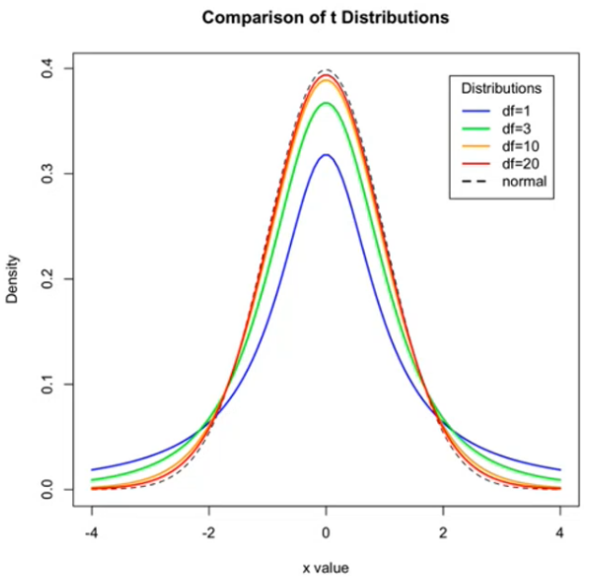
\includegraphics[width=0.6\textwidth]{figdistribuzionit}
    \caption{\small{}}
    \end{figure}
Il $t$ è quindi una famiglia di curve che variano al variare dei gradi di libertà, ovvero alla numerosità del campione.
\\
Quando, con variabili normali, la numerosità del campione aumenta a sufficienza (attorno alle 40-50 unità), il $t$ e la $Z$ restituiscono gli stessi risultati, ovvero il $t$ soglia e la $Z$ soglia tendono a convergere per $n$ elevati (cioè all'aumentare di $n$, $t$ tenderà ad 1.96, per tot gradi di libertà, con un $\alpha$ di 0.05, dato che con $Z$ 1.96 è il valore soglia di $Z$ che taglia a destra e sinistra della curva il 2.5\% della curva sottesa, per un totale del 5\%.).
\\
Al diminuire di $n$, il $t$ soglia è più elevato della $Z$ soglia. Ciò si può intuire a partire dalla figura \ref{fig11.1-1}, nella quale è evidente come, pur essendo simili, la distribuzione di $t$ abbia delle code più alte rispetto alla distribuzione standardizzata:
\begin{figure}[H]\label{fig11.1-1}
    \centering
    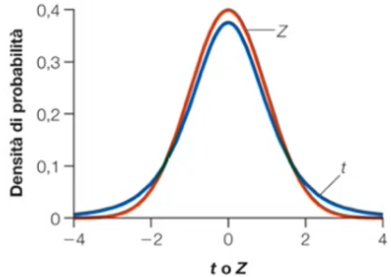
\includegraphics[width=0.6\textwidth]{fig11.1-1}
    \caption{\small{}}
    \end{figure}
Questa differenza è importante, poiché le code sono cruciali nel calcolo degli intervalli di confidenza e nella verifica delle ipotesi.
\\
Ad esempio, il $95\%$ dell'area sottesa dalla curva della distribuzione $t$ con 4 gradi di libertà è compreso tra -2.78 e +2.78 (quindi, estraendo più volte un campione casuale di $n = 5$ da una popolazione normale, nel $95\%$ dei casi la $\overline{Y}$ che si ottiene sarà compresa entro 2.78 errori standard stimati a partire dalla vera media della popolazione, $\mu$).
\\
Rispetto alla distribuzione normale standardizzata ($Z$), invece, il $95\%$ dei casi è compreso tra -1.96 e +1.96; il più ampio intervallo di valori di $t$, rispetto a $Z$, è determinato dal fatto che non si conosce il valore vero dell'errore standard, ma solo una sua stima.
\\
Il valore 2.78 è il valore critico al $5\%$ della distribuzione $t$ con $df = 4$. La percentuale $5\%$ si riferisce all'area sottesa dalle code della distribuzione $t$ (\ref{fig11.1-2}):
\begin{figure}[H]\label{fig11.1-2}
    \centering
    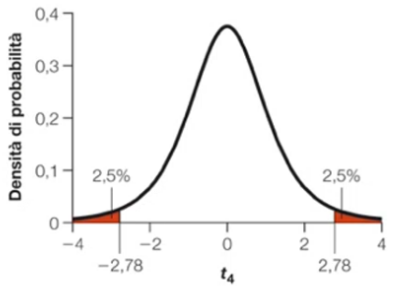
\includegraphics[width=0.6\textwidth]{fig11.1-2}
    \caption{\small{}}
    \end{figure}
Ogni distribuzione di $t$ ha un suo valore critico al $5\%$, che dipende dal numero di gradi di libertà; conoscendo questi, il valore si può rintracciare nella Tavola statistica C (\ref{tavC}).
% come usare la tavola: si identifica la cella che corrisponde alla riga corrispondente al numero di gradi di libertà ed alla colonna corrispondente ad $\alpha(code)=valore\ \alpha$.
\\
Per indicare un valore critico di $t$ si impiega la notazione:
\begin{equation}
    t_{\alpha(code),df}
\end{equation}
Nel caso del valore critico dell'esempio, dunque $t_{0.05(2),4}$.
\\
\\
Il $t$ si basa sulla stima di una media e di una deviazione standard ed assume che vi sia una distribuzione normale (e quindi che la media sia un valore rappresentativo).
\\
Dunque, quello del $t$ di Student è un approccio migliore di quello che utilizza $Z$ quando i parametri sono ignoti ed $n$ è relativamente basso ($<$40-50).

\section{Intervalli di confidenza e \texorpdfstring{$t$}{Lg}}
Lo stesso problema che si riscontra nel confronto tra valori attesi ed osservati si ha nella definizione degli intervalli di confidenza: utilizzare $Z$ non permette di tenere conto del fatto che si sta utlizzando un campione e che quindi non si conosce la variabilità teorica.
\\
Per cacolare gli intervalli di confidenza si utilizza dunque la $t$, e non la $Z$, che comunque corrispondono per $n$ elevati ($>$40-50, quindi usare $t$ per il calcolo degli IC solo per $n$ inferiori). Dunque, quando opportuno, l'\textbf{intervallo di confidenza della media campionaria} si calcola come:
\begin{equation}
    \overline{Y}-t_{\alpha(2),df}ES_{\overline{Y}}\ < \mu <\ \overline{Y}+t_{\alpha(2),df}ES_{\overline{Y}} 
\end{equation}
In questo caso, il parametro di riferimento è la media ($\mu$), ed i gradi di libertà sono $n-1$.
\subsection{\texorpdfstring{$t$}{Lg} test per un campione}
Per verificare le ipotesi sulle medie delle popolazioni è stata sviluppata una serie di $t$ test, tra cui il \textbf{$t$ test per un campione}, utile per confrontare la media di un singolo campione con uno specifico valore della media della popolazione definito dall'ipotesi nulla.
\\
Dunque, le ipotesi sono:
\begin{itemize} \tightlist
    \item $H_O$: la media campionaria ($\overline{Y}$) non differisce da una media ipotetica ($\mu_0$);
    \item $H_A$: la media campionaria ($\overline{Y}$) differisce da una media ipotetica ($\mu_0$).
\end{itemize}
Il test è a due code, poiché l'ipotesi alternativa prevede sia i casi in cui la media campionaria è più grande, sia quelli in cui essa è più piccola della media ipotetica.
\\
Se si dovesse verificare l'ipotesi nulla, si potrebbe impiegare il $t$ test per un campione per determinare se la $\overline{Y}$ calcolata a partire da un campione sia sufficientemente diversa da zero per poter giustificare il rifiuto dell'ipotesi nulla.
\\
Si può poi calcolare il P-value per il test confrontando la $t$ osservata con la distribuzione $t$ di Student.
\begin{example}[temperatura corporea]
    La temperatura corporea dell'uomo è pari a 98.6\textdegree F.
    Le ipotesi sono:
    \begin{itemize} \tightlist
        \item $H_O$: la temperatura corporea dell'uomo è di 98.6\textdegree F;
        \item $H_A$: la temperatura corporea dell'uomo non è di 98.6\textdegree F.
    \end{itemize}
    Si analizzano 25 soggetti sani e si ottengono $\overline{Y} = 98.524$ ed $s = 0.678$.
    \\
    Per prima cosa si dovrebbe plottare la distribuzione di frequenza della temperatura dei 25 soggetti e vedere se questa è grossomodo normale:
    \begin{figure}[H]\label{fig11.3-1}
        \centering
        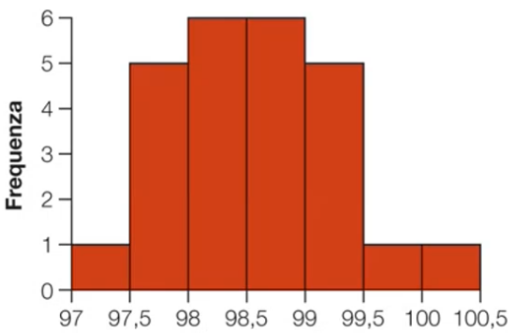
\includegraphics[width=0.6\textwidth]{fig11.3-1}
        \caption{\small{Frquenza assoluta, dato che sull'asse delle y è riportato il conteggio}}
    \end{figure}
    La media della temperatura osservata differisce significativamente dalla media attesa?
    \\
    Per poter ottenere $t$, si calcola $ES_{\overline{Y}}$:
    \begin{equation}
        ES_{\overline{Y}} = \frac{s}{\sqrt{n}} = \frac{0.678}{\sqrt{25}} = 0.1356
    \end{equation}
    Dunque:
    \begin{equation}
        t = \frac{\overline{Y}-\mu_0}{ES_{\overline{Y}}} = \frac{98.524-98.6}{0.1356} = -0.56
    \end{equation}
    Un accordo perfetto tra dati ed ipotesi nulla implicherebbe una media campionaria pari a quella teorica, e $t=0$. Ci si deve chiedere, dunque, se il valore $t=-0.56$ ottenuto è sufficientemente diverso da zero da poter rifiutare l'ipotesi nulla.
    \\
    Alla domanda si può rispondere calcolando il P-value al computer, oppure utilizzando la Tavola statistica C (\ref{tavC}).
    \\
    \\
    \underline{\textit{Con software}}
    \\
    Il P-value rappresenta la probabilità di ottenere un risultato altrettanto o più estremo di $t=-0.56$, assumendo vera l'ipotesi nulla; tale probabilità è rappresentata dall'area sottesa dalla curva della distribuzione $t$ in figura \ref{fig11.3-2}:
    \begin{figure}[H]\label{fig11.3-2}
        \centering
        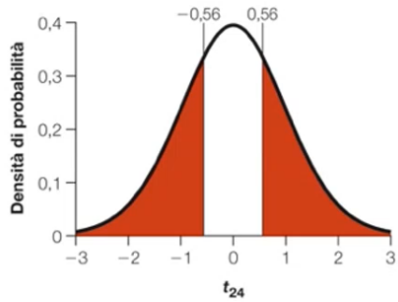
\includegraphics[width=0.6\textwidth]{fig11.3-2}
        \caption{\small{}}
    \end{figure}
    Nella probabilità sono incluse entrambe le code della distribuzione $t$, essendo il test a due code.
    \\
    Il P-value è dato da:
    \begin{equation}
        P = Pr[t<-0.56]+Pr[t>0.56]
    \end{equation}
    E, data la simmetria della distribuzione:
    \begin{equation}
        P = 2Pr[t>0.56]
    \end{equation}
    Con un programma si calcola che $P = 0.58$ e, poiché tale valore è maggiore di 0.05, non si rifiuta l'ipotesi nulla.
    \\
    \\
    \underline{\textit{Con la tavola statistica}}
    \\
    La probabilità che serve, Pr[t<-0.56 o t>0.56], non è riportata direttamente, ma si possono ricavare i valori critici di $t$ per diversi valori di $\alpha$. 
    \\
    Il valore critico di una statistica test identifica il punto o i punti nella sua distribuzione che hanno una certa probabilità $\alpha$ nelle sue code.
    \\
    I valori della statistica test più estremi nelle code hanno P-value minori di $\alpha$, quindi, se il valore di $t$ dista da zero più di quanto non disti il valore critico, allora si può rifiutare l'ipotesi nulla, mentre se il valore calcolato di $t$ è più vicino a zero del valore critico, l'ipotesi nulla non si può rifiutare.
    \\
    Il valore critico di $t$ corrispondente ad $\alpha(2) = 0.05$ ed a 24 gradi di libertà (dato che $df = n-1$) è:
    \begin{equation}
        t_{0,05(2),24} = 2.06
    \end{equation}
    Tale valore definisce il 5\% delle probabilità nelle code della distribuzione $t$, con il 2.5\% in ciascuna di esse per un test a due code. Dunque, il 5\% dell'area sottesa dalla curva $t$ con 24 gradi di libertà si trova all'esterno degli estremi -2.06 e 2.06; mentre il valore di $t$ calcolato, 0.56, è interno a tale intervallo, perciò non ricade in una delle due code, e l'ipotesi nulla non può essere rifiutata.
    \\
    \\
    L'intervallo di valori della temperatura corporea media più plausibile in base ai dati si può ottenere calcolando l'intervallo di confidenza al 95\%:
    \begin{align}
        \overline{Y}-t_{\alpha(2),df}ES_{\overline{Y}}\ < &\mu_0 <\ \overline{Y}+t_{\alpha(2),df}ES_{\overline{Y}}
        \\
        \Rightarrow \quad 98.524-2.06(0.1356)<&\mu_0<98.524+2.06(0.1356)
        \\
        \Rightarrow \quad 98.24<&\mu_0<98.80
    \end{align}
    Se si avesse a disposizione una dimensione campionaria maggiore, l'errore di campionamento diminuirebbe; quindi, con campioni più grandi, la probabilità di rifiutare un'ipotesi nulla quando essa è falsa è maggiore, e campioni più piccoli potrebbero portare ad errori di tipo II.
\end{example}
\begin{example}[guida distratta]\label{esguida}
    Dieci persone vengono osservate alla guida in due casi, con il cellulare e dopo aver bevuto due birre. La media teorica è 73.8 ($\mu_0$). Nella tabella \ref{tabguida} sono riportati l'identificativo di ogni soggetto (il soggetto uno per il cellulare e quello per la birra sono persone diverse, e così via) ed il numero di birilli fatto cadere in entrambi i casi:
    \begin{table}[H]
        \centering
        \renewcommand\arraystretch{1.2}
        \begin{tabular}{c|c|c}
        \hline
        \textbf{ID}& \textbf{Cellulare} & \textbf{Birra}\\
        \hline
        \textbf{1} & 14 & 28\\
        \hline
        \textbf{2} & 44 & 36\\
        \hline
        \textbf{3} & 17 & 38\\
        \hline
        \textbf{4} & 69 & 42\\
        \hline
        \textbf{5} & 77 & 57\\
        \hline
        \textbf{6} & 80 & 60\\
        \hline
        \textbf{7} & 82 & 80\\
        \hline
        \textbf{8} & 86 & 81\\
        \hline
        \textbf{9} & 99 & 83\\
        \hline
        \textbf{10} & 99 & 91\\
        \hline
        \end{tabular}
        \caption{\small{}}
        \label{tabguida}
    \end{table}\noindent
    Da fare:
    \begin{itemize} \tightlist
        \item confrontare le medie ottenute con quelle attese (usando i valori attesi di $t$);
        \item calcolare IC95\% per i due risultati dei test;
        \item se $n = 20$ invece di 10, cambierebbe qualcosa?
    \end{itemize}
    Si calcolano i valori delle medie campionarie rispettive ai due casi (cellulare e birra):
    \begin{equation}
        \overline{Y}_{cell} = \frac{14+44+17+69+77+80+82+86+99+99}{10} = 66.7
    \end{equation}
    \begin{equation}
        \overline{Y}_{birra} = \frac{28+36+38+42+57+60+80+81+83+91}{10} = 59.6
    \end{equation}
    Si calcolano le deviazioni standard campionarie, necessarie per ottenere gli errori standard, che servono per il calcolo della $t$:
    \begin{equation}
        s_{cell} = \sqrt{\frac{\sum\limits_1^n{(Y_i - \overline{Y})^2}}{n-1}} = 
    \end{equation}
    \begin{equation}
        s_{birra} = \sqrt{\frac{\sum\limits_1^n{(Y_i - \overline{Y})^2}}{n-1}} = 
    \end{equation}
    Dunque:
    \begin{equation}
        ES_{\overline{Y}_{cell}} = \frac{s}{\sqrt{n}} = \frac{}{\sqrt{10}} = 
    \end{equation}
    \begin{equation}
        ES_{\overline{Y}_{birra}} = \frac{s}{\sqrt{n}} = \frac{}{\sqrt{10}} = 
    \end{equation}
    Dunque:
    \begin{equation}
        t_{cell} = \frac{\overline{Y}-\mu_0}{ES_{\overline{Y}}} = 
    \end{equation}
    \begin{equation}
        t_{birra} = \frac{\overline{Y}-\mu_0}{ES_{\overline{Y}}} = 
    \end{equation}
    I risultati dei calcoli prececdenti sono riportati nella tabella \ref{tabguida2}:
    \begin{table}[H]
        \centering
        \renewcommand\arraystretch{1.2}
        \begin{tabular}{c|c|c}
        \hline
        & \textbf{Cellulare} & \textbf{Birra}\\
        \hline
        \textbf{$\overline{Y}$} & 66.70 & 59.60\\
        \hline
        \textbf{$s$} & 31.17 & 22.96\\
        \hline
        \textbf{$ES$} & 9.86 & 7.26\\
        \hline
        \textbf{$t$} & -0.720 & -1.955\\
        \hline
        \end{tabular}
        \caption{\small{}}
        \label{tabguida2}
    \end{table}\noindent
    A questo punto, solitamente, si dovrebbe ricavare il valore critico di $t$ per $\alpha(2) = 0.05$ e confrontarlo con i valori di $t$ calcolati; tuttavia, dal momento che il valore minimo che $t$ può assumere con $\alpha = 0.05$ è 1.96, e dato che entrambi i valori di $t$ ottenuti sono inferiori a tale numero, si può direttamente affermare che le differenze tra le medie osservate e quella teorica non sono significative, e quindi non si rifiuta l'ipotesi nulla.
    \\
    Gli intervalli di confidenza per i due casi sono:
    \begin{align}
        \overline{Y}_{cell}-t_{\alpha(2),df}ES_{\overline{Y}_{cell}}\ < &\mu_0 <\ \overline{Y}_{cell}+t_{\alpha(2),df}ES_{\overline{Y}_{cell}}
        \\
        \Rightarrow \quad 66.7-0.720(9.86)<&\mu_0<66.7+0.720(9.86)
        \\
        \Rightarrow \quad 59.6<&\mu_0<73.8
    \end{align}
    \begin{align}
        \overline{Y}_{birra}-t_{\alpha(2),df}ES_{\overline{Y}_{birra}}\ < &\mu_0 <\ \overline{Y}_{birra}+t_{\alpha(2),df}ES_{\overline{Y}_{birra}}
        \\
        \Rightarrow \quad 59.6-1.955(7.26)<&\mu_0<59.6+1.955(7.26)
        \\
        \Rightarrow \quad 45.41<&\mu_0<73.79
    \end{align}
    Nel caso in cui $n$ \colorbox{lyellow}{fosse 20}
\end{example}

\chapter{Confronto tra due medie}
Si riprende l'esempio \ref{esguida}. Se entrambi i test (cellulare e birra) venissero svolti da una stessa persona (ovvero se ciascun ID facesse riferimento ad un unico individuo, che ha svolto il test di guida in entrambe le condizioni), ci si potrebbe chiedere se, nonostante le medie osservate non differiscano significativamente dalla media teorica, ciascun individuo mostri una differenza significativa tra le performance rispettive alle due diverse condizioni.
\\
Alle due tabelle precedenti si aggiunge il campo "Delta" (tabella \ref{tabguida3}):
\begin{table}[H]
    \centering
    \renewcommand\arraystretch{1.2}
    \begin{tabular}{c|c|c||c}
    \hline
    \textbf{ID}& \textbf{Cellulare} & \textbf{Birra} & \textbf{Delta}\\
    \hline
    \textbf{1} & 14 & 28 & 14\\
    \hline
    \textbf{2} & 44 & 36 & -8\\
    \hline
    \textbf{3} & 17 & 38 & 21\\
    \hline
    \textbf{4} & 69 & 42 & -27\\
    \hline
    \textbf{5} & 77 & 57 & -20\\
    \hline
    \textbf{6} & 80 & 60 & -20\\
    \hline
    \textbf{7} & 82 & 80 & -2\\
    \hline
    \textbf{8} & 86 & 81 & -5\\
    \hline
    \textbf{9} & 99 & 83 & -16\\
    \hline
    \textbf{10} & 99 & 91 & -8\\
    \hline
    \hline
    \textbf{$\overline{Y}$} & 66.70 & 59.60 & -7.10\\
    \hline
    \textbf{$s$} & 31.17 & 22.96 & 15.18\\
    \hline
    \textbf{$ES$} & 9.86 & 7.26 & 4.80\\
    \hline
    \textbf{$\mu_0$} & 73.8 & 73.8 & 0\\
    \hline
    \textbf{$t$} & -0.720 & -1.955 & -1.479\\
    \hline
    \end{tabular}
    \caption{\small{}}
    \label{tabguida3}
\end{table}\noindent
I valori delta corrispondono alla differenza tra i valori corrispondenti alle due condizioni.
\\
Se la performance con il cellulare e quella con la birra fossero uguali, la differenza tra i due valori dovrebbe essere pari a zero, quindi la media teorica è pari a zero.
\\
Per rispondere alla domanda si devono quindi confrontare la media osservata ($\overline{Y}_{delta}$), con la media attesa ($\mu_{delta}$), seguendo lo stesso procedimento dell'esempio di riferimento.
\\
Il valore di $t$ che si ottiene è nuovamente inferiore ad 1.96, quindi le performance sotto le due possibili condizioni non sono significativamente differenti; questo, almeno, se si considera il test come avente due code. Tuttavia, in questo caso, è ragionevole supporre che il test sia ad una coda, dato che è improbabile che stando al cellulare o bevendo birra la guida addirittura migliori; \colorbox{lyellow}{\parbox{0.98\textwidth}{per questo, l'$\alpha$ da considerare è 0.1 (ovvero 0.05 per ciascuna coda); il $t$ di riferimento sarà dunque più basso rispetto al caso che prevede due code, il che vuol dire che il test è in grado di rilevare anche differenze più piccole tra le due medie che si mettono a confronto, il che è dovuto al fatto che c'è un vincolo in meno imposto dal disegno sperimentale.
\\
lezione 20211201}}

\section{Disegno sperimentale per dati appaiati o indipendenti}

Quando si confrontano due gruppi si può organizzare il disegno sperimentale in due modi:
\begin{itemize} \tightlist
    \item \textbf{per dati indipendenti}: ogni gruppo di trattamento è costituito da un campione casuale indipendente di unità (si hanno due gruppi di dati indipendenti);
    \item \textbf{per dati appaiati} (o dipendenti): si applicano entrambi i trattamenti a ciascuna unità campionaria (si ha un gruppo di dati appaiati, si ha uno stesso numero nei due gruppi ed esiste una univocità tra ciascun valore del primo gruppo ed i corrispondenti del secondo).
\end{itemize}
Un disegno sperimentale per dati appaiati è più robusto, poiché permette di controllare gli effetti della variabilità tra le unità campionarie che non hanno a che fare con il trattamento d'interesse.
\\
In alcuni casi, comunque, è impossibile disporre di dati appaiati.
\\
In caso di disegno sperimentale per dati appaiati, da applicare su un campione in cui ogni unità campionaria è un individuo, e ciò che si misura è la performance di ciscuno in una task prima e dopo un trattamento, è necessario evitare bias da apprendimento, misurando le performance dopo diverse prove di allenamento.

\section{Confronto appaiato di medie}

In tal caso, pur essendo appaiati i dati, le unità campionarie che si mettono a confronto sono differenti; l'appaiamento, dunque, non impone che si misuri sulle stesse unità campionarie.
\begin{example}[merlo alirosse]\label{esmerlo}
    C'è un'associazione positiva tra livelli di testosterone e fitness riproduttiva, ma il testosterone riduce la risposta immunitaria.
    \\
    Questo è vero anche nel merlo alirosse (ovvero, i merli alirosse maschi che hanno più fitness hanno anche una ridotta risposta immunitaria)?
    \\
    A 13 maschi si somministra testosterone e se ne controllano gli anticorpi prima e dopo la somministrazione.
    \\
    Le ipotesi sono:
    \begin{itemize} \tightlist
        \item $H_0$: la produzione di anticorpi non cambia dopo la somministrazione di testosterone;
        \item $H_A$: la produzione di anticorpi cambia dopo la somministrazione di testosterone.
    \end{itemize}
    Nell'esempio, i dati sono appaiati, e si effettuano misure sulle stesse unità campionarie (stesso individuo, prima e dopo la somministrazione).
    \\
    I risultati sono rappresentati nello scatterplot in Figura \ref{fig12.2-1}:
    \begin{figure}[H]\label{fig12.2-1}
        \centering
        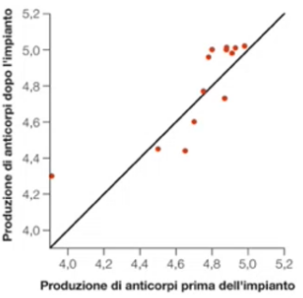
\includegraphics[width=0.6\textwidth]{fig12.2-1}
        \caption{\small{}}
    \end{figure}
    Si devono calcolare le differenze tra le coppie di dati, stimare media e varianza delle differenze e stimare l'IC 95\%.
    \\
    Gli intervalli di confidenza per le differenze medie tra dati appaiati si calcolano come:
    \begin{equation}
        \overline{d}-t_{\alpha(2),df}ES_{\overline{d}}<\mu_d<\overline{d}+t_{\alpha(2),df}ES_{\overline{d}}
    \end{equation}
    In cui:
    \begin{equation}
        ES_{\overline{d}} = \frac{s_{\overline{d}}}{\sqrt{n}}
    \end{equation}
    È l'errore standard della differenza della media.
    \\
    Ciò che bisogna stabilire è se tale intervallo include o meno lo zero; se lo include, l'ipotesi nulla non può essere rifiutata.
    \\
    Nell'ipotesi corrente, l'intervallo include lo zero, e dunque non è possibile rifiutare l'ipotesi nulla. I dati disponibili, quindi, non permettono di evidenziare una differenza tra i dati confrontati.
    \\
    In alternativa all'impiego dell'IC 95\%, si può effettuare un $t$ test:
    \begin{equation}
        t_{df} = \frac{\overline{d}-\mu_{d0}}{ES_{\overline{d}}}
    \end{equation}
    In questo caso, il test è a due code e, con un $t$ calcolato pari a -1.27, non si può rifiutare l'ipotesi nulla.
\end{example}
\clearpage
\begin{example}[amputazione dei pedipalpi]\label{esamputazione}
    I dati sulla velocità di ragni prima e dopo l'amputazione dei pedipalpi sono riportati nella tabella \ref{tabamputazione}:
    \begin{table}[H]
        \centering
        \renewcommand\arraystretch{1.2}
        \begin{tabular}{c|c|c}
        \hline
        \textbf{ID} & \textbf{prima} & \textbf{dopo}\\ 
        \hline
        \textbf{1} & 1.25 & 2.40\\
        \hline
        \textbf{2} & 1.64 & 5.06\\
        \hline
        \textbf{3} & 1.91 & 3.40\\
        \hline
        \textbf{4} & 2.31 & 2.32\\
        \hline
        \textbf{5} & 2.37 & 5.45\\
        \hline
        \textbf{6} & 2.38 & 4.49\\
        \hline
        \textbf{7} & 2.84 & 4.94\\
        \hline
        \textbf{8} & 2.87 & 3.52\\
        \hline
        \textbf{9} & 2.93 & 3.31\\
        \hline
        \textbf{10} & 2.94 & 3.50\\
        \hline
        \textbf{11} & 2.98 & 3.70\\
        \hline
        \textbf{12} & 3.00 & 3.22\\
        \hline
        \textbf{13} & 3.09 & 3.17\\
        \hline
        \textbf{14} & 3.22 & 3.22\\
        \hline
        \textbf{15} & 3.41 & 5.26\\
        \hline
        \textbf{16} & 3.55 & 4.70\\
        \hline
        \end{tabular}
        \caption{\small{}}
        \label{tabamputazione}
    \end{table}\noindent
    Da fare:
    \begin{itemize} \tightlist
        \item calcolare IC 95\% della differenza tra prima e dopo;
        \item calcolare $t$ e livello di significatività.
    \end{itemize}
    Le ipotesi sono:
    \begin{itemize} \tightlist
        \item $H_0$: l'amputazione dei pedipalpi non influisce sulla velocità dei ragni;
        \item $H_A$: l'amputazione dei pedipalpi influisce sulla velocità dei ragni.
    \end{itemize}
    Per poter ottenere i valori di $t$, si calcolano la media campionaria, la deviazione standard campionaria e l'errore standard campionario relativi ai due casi, prima e dopo, e alla differenza tra essi, delta, che si ottiene sottraendo i valori relativi alla colonna "prima" a quelli della colonna "dopo"; i risultati ottenuti sono riportati nella tabella \ref{tabamputazione2}:
    \begin{table}[H]
        \centering
        \renewcommand\arraystretch{1.2}
        \begin{tabular}{c|c|c||c}
        \hline
        \textbf{ID} & \textbf{prima} & \textbf{dopo} & \textbf{delta}\\ 
        \hline
        \textbf{1} & 1.25 & 2.40 & 1.15\\
        \hline
        \textbf{2} & 1.64 & 5.06 & 3.42\\
        \hline
        \textbf{3} & 1.91 & 3.40 & 1.49\\
        \hline
        \textbf{4} & 2.31 & 2.32 & 0.01\\
        \hline
        \textbf{5} & 2.37 & 5.45 & 3.08\\
        \hline
        \textbf{6} & 2.38 & 4.49 & 2.11\\
        \hline
        \textbf{7} & 2.84 & 4.94 & 2.1\\
        \hline
        \textbf{8} & 2.87 & 3.52 & 0.65\\
        \hline
        \textbf{9} & 2.93 & 3.31 & 0.38\\
        \hline
        \textbf{10} & 2.94 & 3.50 & 0.56\\
        \hline
        \textbf{11} & 2.98 & 3.70 & 0.72\\
        \hline
        \textbf{12} & 3.00 & 3.22 & 0.22\\
        \hline
        \textbf{13} & 3.09 & 3.17 & 0.08\\
        \hline
        \textbf{14} & 3.22 & 3.22 & 0\\
        \hline
        \textbf{15} & 3.41 & 5.26 & 1.85\\
        \hline
        \textbf{16} & 3.55 & 4.70 & 1.15\\
        \hline
        \hline
        \textbf{$\overline{Y}$} & 2.67 & 3.85 & 1.19\\
        \hline
        \textbf{$s$} & 0.64 & 0.99 & 1.07\\
        \hline
        \textbf{$ES$} & 0.160 & 0.248 & 0.268\\
        \hline
        \textbf{$\mu_0$} & ? & ? & 0\\
        \hline
        \textbf{$t$} & ? & ? & 4.44\\
        \hline
        \end{tabular}
        \caption{\small{}}
        \label{tabamputazione2}
    \end{table}\noindent
    Per determinare il livello di significatività si ricorre alla Tavola statistica C (\ref{tavC}); a partire da essa, si ricava il valore critico di $t$ per $\alpha = 0.05$:
    \begin{equation}
        t_{0.05(2),15} = 2.13
    \end{equation}
    Siccome il $t$ calcolato non ricade nell'intervallo tra -2.13 e 2.13, $P>0.05$, e si può rifiutare l'ipotesi nulla.
    \\
    Per quanto riguarda l'intervallo di confidenza, questo si definisce utilizzando il valore $t_{0.05(2),15}$:
    \begin{align*}
        \overline{d}-t_{\alpha(2),df}ES_{\overline{d}}<\ &\mu_d<\overline{d}+t_{\alpha(2),df}ES_{\overline{d}}
        \\
        \Rightarrow \quad 0.62<\ &\mu_d<1.76
    \end{align*}
    Dato che tale intervallo non include il valore calcolato di $t$, si può affermare che la differenza tra le medie delle velocità misurate prima e dopo l'amputazione risulta significativa, e dunque si può rifiutare l'ipotesi nulla.
    Tutte le formule utilizzate nell'esercizio sono le stesse impiegate nell'esercizio \ref{esmerlo}.
\end{example}

\section{Confronto tra medie di dati indipendenti}
\subsection{Per due gruppi indipendenti con varianze omogenee}
Si hanno due gruppi ma nessun modo di appaiare il valore relativo ad un caso di un gruppo con un valore di un caso dell'altro gruppo.
\begin{example}[funzione delle spine cefaliche dei frinosomi]\label{esfrinosomi}
    I frinosomi sono rettili con spine cutanee. Tali spine hanno una funzione che riguarda la dimensione intraspecifica o quella interspecifica?
    \\
    Le averle sono uccelli che predano anche i frinosomi, impalandoli su spine di piante.
    \\
    Nell'area di studio, dei ricercatori hanno raccolto tutte le teste di frinosomi che erano state impalate dalle averle, poi hanno catturato dei frinosomi in vita ed hanno misurato la lunghezza delle spine degli individui vivi e di quelli morti.
    \\
    Le ipotesi sono:
    \begin{itemize} \tightlist
        \item $H_0$: le spine degli animali predati e di quelli vivi hanno eguali lunghezze;
        \item $H_0$: le spine degli animali predati e di quelli vivi non hanno eguali lunghezze;
    \end{itemize}
    Sono stati campionati 30 animali predati e 154 vivi; i dati raccolti sono rappresentati nei grafici in Figura \ref{fig12.3-1}:
    \begin{figure}[H]\label{fig12.3-1}
        \centering
        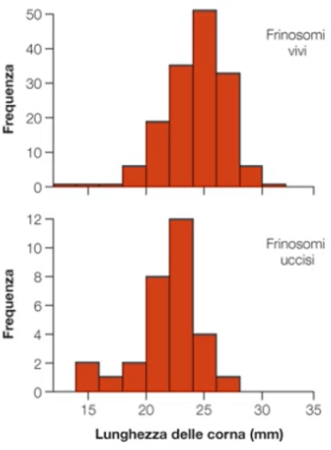
\includegraphics[width=0.6\textwidth]{fig12.3-1}
        \caption{\small{}}
    \end{figure}
    Dai grafici, i soggetti vivi sembrano avere spine cefaliche leggermete più lunghe rispetto ai predati.
    \\
    Lo sbilanciamento tra $n_{vivi}$ ed $n_{predati}$ potrebbe essere problematico.
    \\
    In questo caso, si hanno due gruppi di misurazione, con dati indipendenti.
    \\
    Si calcola la statistica $t$:
    \begin{equation}
        t = \frac{\overline{Y}_1-\overline{Y}_2}{ES_{\overline{Y}_1-\overline{Y}_2}}
    \end{equation}
    In cui:
    \begin{equation}
        ES_{\overline{Y}_1-\overline{Y}_2} = \sqrt{s_p^2(\frac{1}{n_1}+\frac{1}{n_2})}
    \end{equation}
    La grandezza $s_p^2$ è detta \textbf{varianza campionaria comune} (pooled, in inglese, da cui la p); si tratta della media pesata (o ponderata) delle varianze campionarie nei due gruppi, $s_1^2$ e $s_2^2$:
    \begin{equation}
        s_p^2 = \frac{df_1 s_1^2+df_2 s_2^2}{df_1+df_2}
    \end{equation}
    In cui:
    \begin{equation}
        df_1 = n_1-1
    \end{equation}
    E:
    \begin{equation}
        df_2 = n_2-1
    \end{equation}
    Nell'esempio, il $t$ calcolato è pari a 4.35; dato che il valore critico è $t_{0.05(2),182} = 1.97$, si rifiuta l'ipotesi nulla.
    \\
    Il test è a due code perché non si può escludere che gli animali con le spine più grandi vengano predati più degli altri.
    \\
    L'intervallo di confidenza relativo alla differenza tra le medie campionarie è:
    \begin{align*}
        \overline{Y}_1-\overline{Y}_2-t_{\alpha(2),df}ES_{\overline{Y}_1-\overline{Y}_2}<\ &\mu_1-\mu_2<\overline{Y}_1-\overline{Y}_2+t_{\alpha(2),df}ES_{\overline{Y}_1-\overline{Y}_2}
        \\
        \Rightarrow \quad 1.25<\ &\mu_1-\mu_2<3.33
    \end{align*}
    Dunque, anche in questo caso si possono usare gli IC, anche se il $t$ test è più potente e preciso.
\end{example}

\subsection{Per due gruppi indipendenti con varianze non omogenee}

Un'assunzione importante del test $t$ per due campioni è che le deviazioni standard delle due popolazioni siano uguali. Se questa assunzione non è soddisfatta, allora si dovrebbe usare il \textbf{test $t$ approssimato di Welch}. Il test di Welch è simile al test t per due campioni, ad eccezione del fatto che l'errore standard e i gradi di libertà vengono calcolati in modo diverso.
\\
Il test di Welch può essere usato anche quando le varianze nei due gruppi sono diverse.
\\
La distribuzione della $t$ di Welch sotto l'ipotesi nulla corrisponde con la distribuzione $t$, ma il numero di gradi di libertà è minore, rispetto a quello del test $t$ per due campioni:
\begin{equation}
    df = \frac{(\frac{s_1^2}{n_1}+\frac{s_2^2}{n_2})^2}{\frac{(\frac{s_1^2}{n_1})^2}{n_1-1}+\frac{(\frac{s_2^2}{n_2})^2}{n_2-1}}
\end{equation}
La $t$ approssimata di Welch è pari a:
\begin{equation}
    t = \frac{(\overline{Y_1}-\overline{Y_2})-(\mu_1-\mu_2)_0}{\sqrt{\frac{s_1^2}{n_1}+\frac{s_2^2}{n_2}}}
\end{equation}
\begin{example}[specie alloctone]\label{essalmoni}
In uno studio è stata analizzata la sopravvivenza di una specie autoctona, il salmone reale, in una serie di corsi d'acqua, in alcuni dei quali era stato introdotto il salmerino di Fonte, una specie alloctona, con l'obiettivo di determinare se la presenza di quest'ultimo potesse influenzare la sopravvivenza del salmone.
\\
I dati sono riassunti nella tabella \ref{tabsalmoni}:
\begin{table}[H]
    \centering
    \renewcommand\arraystretch{1.2}
    \begin{tabular}{c|c|c|c}
    \hline
    \textbf{Salmerino} & \textbf{\makecell{Numero di salmoni\\liberati}} & \textbf{\makecell{Numero di salmoni\\sopravvissuti}} & \textbf{\makecell{Proporzione di salmoni\\sopravvissuti}}\\ 
    \hline
    presente & 820 & 166 & 0.202\\
    \hline
    presente & 960 & 136 & 0.142\\
    \hline
    presente & 700 & 153 & 0.219\\
    \hline
    presente & 545 & 103 & 0.189\\
    \hline
    presente & 769 & 173 & 0.225\\
    \hline
    presente & 1001 & 188 & 0.188\\
    \hline
    assente & 467 & 180 & 0.385\\
    \hline
    assente & 959 & 178 & 0.186\\
    \hline
    assente & 1029 & 326 & 0.317\\
    \hline
    assente & 27 & 7 & 0.259\\
    \hline
    assente & 998 & 120 & 0.120\\
    \hline
    assente & 936 & 135 & 0.120\\
    \hline
    \textbf{Totale} & 9211 & 1865 & \\
    \hline
    \end{tabular}
    \caption{\small{}}
    \label{tabsalmoni}
\end{table}\noindent
Il conteggio dei pesci per trattamento è riportato nella tabella 2x2 \ref{tabsalmoni2}:
\begin{table}[H]
    \centering
    \renewcommand\arraystretch{1.2}
    \begin{tabular}{c|c|c}
    \hline
    & \textbf{\makecell{Salmierino assente}} & \textbf{\makecell{Salmierino presente}}\\ 
    \hline
    \textbf{Sopravvissuti} & 0.194 & 0.0297\\
    \hline
    \textbf{Non sopravvissuti} & 0.235 & 0.1036\\
    \hline
    \end{tabular}
    \caption{\small{}}
    \label{tabsalmoni2}
\end{table}\noindent
Per raggiungere l'obiettivo si potrebbe pensare di utilizzare un test $\chi^2$ di contingenza per valutare l'associazione fra trattamento e sopravvivenza; tuttavia, i salmoni analizzati non sono un campione casuale; infatti, questi sono divisi in gruppi corrispondenti ai corsi d'acqua in cui sono stati liberati. se esiste qualche differenza intrinseca tra i corsi d'acqua per quanto riguarda la sopravvivenza dei salmoni, anche senza considerare gli eventuali effetti della presenza del salmerino, allora due salmoni immessi nello stesso corso d'acqua avranno una probabilità di sopravvivenza simile rispetto a due salmoni presi a caso. considerare tutti i salmoni e condurre l'analisi con una tabella di contingenza porterebbe a commettere un errore di pseudoreplicazione.
\\
Ciò si evita considerando che le unità campionarie indipendenti non sono i salmoni, ma i fiumi; le unità campionarie sono quindi i 12 corsi d'acqua, sei per ogni trattamento. Quindi, i destini di tutti i salmoni in un corso d'acqua vengono riassunti in un'unica misura, la frazione di salmoni sopravvissuti.
\\
Non si confrontano più frequenze assolute in categorie, ma differenze tra le medie di una variabile numerica. Bisogna dunque utilizzare un test per due campioni sulla differenza tra le medie.
\\
I corsi d'acqua in cui sono presenti i salmerini vengono chiama ti gruppo 1, mentre quelli in cui sono assenti vengono chiamati gruppo 2.
\\
Le ipotesi sono:
\begin{itemize} \tightlist
\item $H_0$: la proporzione media di salmoni sopravvissuti è la stessa nei corsi d'acqua con e senza salmerini ($\mu_1 = \mu_2$);
\item $H_A$: la proporzione media di salmoni sopravvissuti è diversa nei corsi d'acqua con e senza salmerini ($\mu_1 \neq \mu_2$)
\end{itemize}
le medie campionarie e le deviazioni standard sono riportate nella tabella \ref{tabsalmoni3}:
\begin{table}[H]
    \centering
    \renewcommand\arraystretch{1.2}
    \begin{tabular}{c|c|c|c}
    \textbf{Gruppo} & \textbf{\makecell{Media campionaria}} & \textbf{\makecell{Deviazione standard\\campionaria ($s_i$)}} & \textbf{\makecell{Dimensione\\campionaria ($n_i$)}}\\ 
    \hline
    salmierini presenti & 0.194 & 0.0297 & 6\\
    \hline
    salmierini assenti & 0.235 & 0.1036 & 6\\
    \hline
    \end{tabular}
    \caption{\small{}}
    \label{tabsalmoni3}
\end{table}\noindent
Gli intervalli di confidenza al 95\% sono presentati accanto ai dati nella figura \ref{fig12.4-1}:
\begin{figure}[H]\label{fig12.4-1}
    \centering
    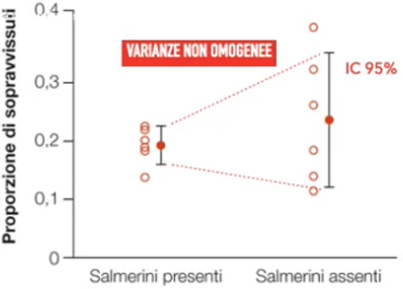
\includegraphics[width=0.6\textwidth]{fig12.4-1}
    \caption{\small{}}
\end{figure}
Tale figura, assieme alle statistiche descrittive riportate nella tabella precedente, mostrano che i corsi d'acqua senza salmerini hanno una deviazione standard circa 3 volte maggiore di quella dei corsi d'acqua con salmerini. Questo è un caso in cui è appropriato utilizzare il test $t$ approssimato di Welch, attraverso il quale, con l'ausilio di un computer, si può calcolare un $P-value$ pari a 0.40. Quindi, dato che $P>0.05$, non si può rifiutare l'ipotesi nulla, il che significa che i dati non dimostrano che i salmerini riducono la sopravvivenza dei salmoni.
\\
L'analisi appropriata, in cui i dati sui salmoni nei corsi d'acqua sono ridotti a un unica misura per ogni corso d'acqua, potrebbe sembrare uno spreco di dati raccolti; tuttavia, riunendo in un'unica misura riassuntiva, come una proporzione, parecchi dati correlati, si ottiene comunque una stima più affidabile del valore vero di tale misura in una data unità campionaria, in questo caso un corso d'acqua.
\end{example}

\section{Errore del confronto diretto}

Un errore che si può commettere quando si confrontano due gruppi e di confrontare la media di ciascun gruppo separatamente con uno stesso valore specificato dalle ipotesi nulla, invece di confrontare direttamente le due medie tra loro punto l'errore potrebbe portare ad una conclusione del tipo "dato che il gruppo uno è significativamente diverso da zero, ma il gruppo 2 non lo è, allora i due gruppi devono essere diversi tra loro". Tale errore è detto \textbf{errore del confronto indiretto}.

\section{Confrontare le varianze}

Spesso è necessario verificare se due popolazioni differiscono nel grado di dispersione delle misure. Due tecniche utili a tale scopo sono il test $F$ ed il test di Levene.

\subsection{Test \texorpdfstring{F}{Lg} per l'uguaglianza delle varianze}

Il \textbf{test $F$} valuta se le varianze di due popolazioni siano uguali; verifica cioè l'ipotesi nulla che $\sigma_1^2 = \sigma_2^2$, contro l'ipotesi che le due varianze siano differenti.
\\
La statistica test $F$ si calcola come rapporto tra le due varianze campionarie:
\begin{equation}
    F = \frac{\sigma_1^2}{\sigma_2^2}
\end{equation}
Se l'ipotesi nulla fosse vera, allora $F$ dovrebbe essere vicino ad 1, discostandosi da 1 soltanto per effetto del caso. Se è vera l'ipotesi nulla, la statistica $F$ ha una distribuzione $F$ con la coppia di gradi di libertà $n_1-1$ ed $n_2-1$. La distribuzione $F$ ha quindi due parametri che specificano i gradi di libertà; il primo numero si riferisce a quelli del numeratore ed il secondo a quelli del denominatore.
\\
Il test $F$ per il confronto tra due varianze assume che la variabile abbia una distribuzione normale in entrambe le popolazioni. Il test è molto sensibile a tale assunzione e dunque non è robusto quando si verifica uno scostamento dei dati dalla condizione di normalità; infatti capita spesso che il test rifiuti erroneamente l'ipotesi nulla di uguaglianza delle varianze quando la distribuzione della variabile in una delle due popolazioni non è normale.

\subsection{Test di Levene per l'omogeneità delle varianze}

Il \textbf{test di Levene} assume che la distribuzione di frequenza delle misure sia circa simmetrica in tutti i gruppi, e funziona molto meglio del test $F$ quando l'assunzione di normalità è violata. Il test di Levene ho anche il vantaggio di poter essere applicato a più di due gruppi, infatti, è in grado di verificare l'ipotesi nulla secondo cui più gruppi hanno tutti la stessa varianza.
\\
Nel test di Levenesi calcola prima il valore assoluto della differenza tra ogni misura è la media campionaria del gruppo. Tali grandezze sono chiamate scarti assoluti. il metodo testa Poi la differenza tra gruppi rispetto alle medie di questi scarti assoluti. La statistica test, $W$, ha anch'essa una distribuzione $F$ sotto l'ipotesi nulla di uguaglianza delle varianze, con la coppia di gradi di libertà $k-1$ per il numeratore e $N-k$ per il denominatore, in cui $k$ è il numero di gruppi (2, nei test a due campioni), ed N è la dimensione campionaria totale ($n_1+n_2$ nel caso di due gruppi).
\\
L'ipotesi nulla viene rifiutata se:
\begin{equation}
    W > F_{\alpha(1),k-1,N-k}
\end{equation}
In cui $F_{\alpha(1),k-1,N-k}$ rappresenta il valore critico della distribuzione $F$.
La statistica test $W$ è pari a:
\begin{equation}
    W = \dfrac{(N-k)\sum_{i=1}^k{n_i(\overline{Z_i}-\overline{Z})^2}}{(k-1)\sum_{i=1}^k\sum_{j=1}^{n_1}{(Z_{ij}-\overline{Z_i})^2}}
\end{equation}
In cui:
\begin{itemize} \tightlist
    \item $Z_{ij} = \abs{Y_{ij}-\overline{Y_i}}$ è il valore assoluto dello scarto tra la singola osservazione $Y_{ij}$ (la j-esima unità dell'i-esimo gruppo) e la media campionaria per il suo gruppo $\overline{Y}_i$ (media campionaria per il gruppo i);
    \item $\overline{Z_i}$ è la media di tutti gli $Z_ij$ per l'i-esimo gruppo;
    \item $\overline{Z}$ è la media generale per tutti gli $Z_ij$, calcolata come media di tutti gli $Z_ij$ raggruppati indipendentemente;
    \item $n_i$ è il numero di osservazioni nell'i-esimo gruppo;
    \item $k$ è il numero di gruppi (2 nel caso dei test a 2 campioni).
\end{itemize} 

\chapter{Violazioni delle assunzioni delle analisi statistiche}

\section{Identificare le violazioni della normalità}

Alcune delle tecniche utili per capire se un insieme di dati numerici sia estratto da una popolazione con una distribuzione normale sono riportati di seguito.

\subsection{Test statistici di normalità}

I test di Shapiro-Wilk (per $n$ < 50) e di Kolmogorov-Smirnoff (per $n$ > 50) possono essere problematici, in quanto con $n$ troppo bassi rischiano di non rilevare una normalità significativa, mentre con $n$ troppo alti potrebbero essere troppo restrittivi nel ritenere come normali distribuzioni che effettivamente potrebbero essere considerate tali; perciò è consigliato\footnote{Il professore consiglia} impiegare tali test solo per casi in cui $n$ è vicino a 50.

\subsubsection{Test di Shapiro-Wilk}

Il test di normalità di Shapiro-Wilk è utilizzabile nei casi in cui n < 50. Il test stima inizialmente la media e la deviazione standard della popolazione usando i dati campionari, poi valuta la bontà con cui una distribuzione normale teorica con quella media e quella deviazione standard si adatta ai dati.

\subsubsection{Test di Kolmogorov-Smirnoff}

Il test di normalità di Shapiro-Wilk è utilizzabile nei casi in cui n > 50. Si tratta di un test più potente di quello di Shapiro-Wilk, ma con esso si ottiene spesso un risultato significativo.

\subsection{Metodi grafici}

Il primo passaggio dell'analisi dei dati dovrebbe sempre essere quello si tracciare un grafico della distribuzione di frequenza ed interpretarlo, dal momento che la dimensione di $n$ può essere fuorviante (Fig. \ref{fig13.1-1}).\\
\begin{figure}[H]
    \centering
    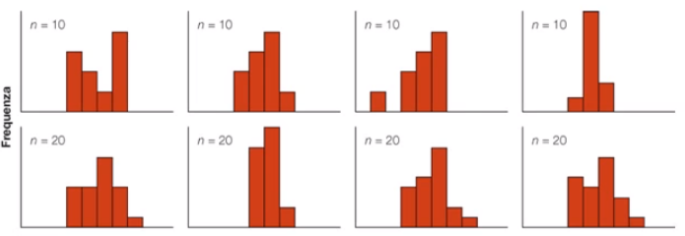
\includegraphics[width=0.6\textwidth]{fig13.1-1}
    \caption{\small{}}
    \label{fig13.1-1}
\end{figure}

Le violazioni della normalità possono presentare diversi gradi di gravità.\\
Quelle riportate in Figura \ref{fig13.1-1} sono considerate violazioni modeste della normalità, e sono tollerate dal t-test e dai test parametrici in generale.

Violazioni più severe sono quelle legate all'asimmetria delle distribuzioni d'interesse (primi tre casi in Fig. \ref{fig13.1-2}).\\
\begin{figure}[H]
    \centering
    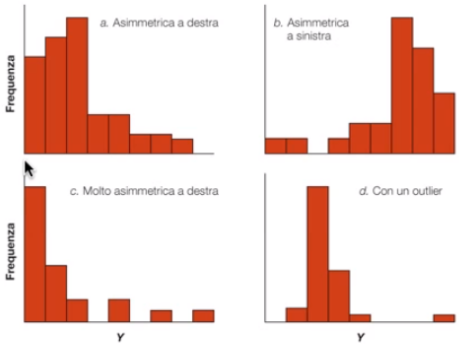
\includegraphics[width=0.6\textwidth]{fig13.1-2}
    \caption{\small{}}
    \label{fig13.1-2}
\end{figure}

Casi del genere possono presentarsi quando i dati hanno valori modesti ed ogni tanto ci sono valori molto elevati (es. carico parassitario in ospiti, spesso modesto, a volte si hanno casi di super-hosts, che determinano asimmetrie nella distribuzione), e non si possono tollerare, per cui si affrontano mediante trasformazione dei dati.

Un'altra situazione è quella di distribuzioni abbastanza simmetriche, che però presentano alcuni casi (in una delle due direzioni o entrambe) che sembrano non appartenere alla distribuzione, degli outliers (caso in basso a destra in Fig. \ref{fig13.1-2}).\\
Mentre i primi tre casi possono essere corretti, il problema degli outlier è più complicato da risolvere, e rende difficile l'impiego di test parametrici, per cui richiede l'impiego di test alternativi, con assunzioni diverse.\\
Stessa cosa quando si hanno variabili ordinali o quando, avendo due gruppi, uno presenta asimmetria a destra e l'altro a sinistra.

\section{Metodi per correggere la violazione della normalità}

\subsection{Trasformazione dei dati}

Le trasformazioni possono essere applicate per migliorare l'adattamento  della distribuzione normale ai dati o, nei casi dei metodi per due campioni (in cui l'assunzione è l'uguaglianza delle deviazioni standard), per rendere le deviazioni standard più simili in gruppi diversi.\\
Quando si applica una trasformazione ad un valore, la stessa deve essere applicata allo stesso modo a tutti i valori di tutti i campioni per quella variabile, per rendere possibile il confronto dei dati (questo è il motivo per cui i casi con due gruppi con asimmetrie opposte sono problematici: applicando una trasformazione si risolvono solo casi con stessa asimmetria).\\
Di seguito sono riportate le trasformazioni più comuni.

\subsubsection{Logaritmica}

Per convertire i dati si usa solitamente il logaritmo naturale:
\begin{equation}
    Y'= ln[Y]
\end{equation}
La trasformazione logaritmica può essere applicata ai dati solo quando tutti i dati sono maggiori di zero, poiché il logaritmo naturale non è definito per valori $\leq 0$. Se i dati comprendono lo zero, si può provare ad impiegare:
\begin{equation}
    Y'= ln[Y+1]
\end{equation}
Generalmente, la trasformazione logaritmica è utile quando:
\begin{itemize} \tightlist
    \item le misure sono rapporti o prodotti di variabili;
    \item la distribuzione di frequenza dei dati è asimmetrica a destra;
    \item il gruppo con la media maggiore (quando si confrontano due gruppi) ha anche la deviazione standard maggiore;
    \item i dati si estendono su più ordini di grandezza.
\end{itemize}

Ad esempio, confrontando le due distribuzioni di probabilità mostrate in Figura \ref{fig13.3-1}:\\
\begin{figure}[H]
    \centering
    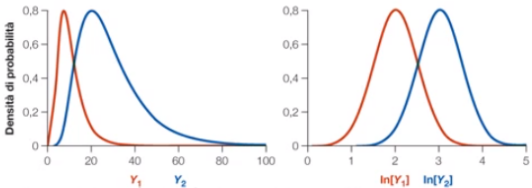
\includegraphics[width=0.6\textwidth]{fig13.3-1}
    \caption{\small{}}
    \label{fig13.3-1}
\end{figure}

Entrambe le curve sono asimmetriche a destra (asimmetria positiva), ed il gruppo con la media più alta ha anche la deviazione standard più alta. La trasformazione logaritmica risolve entrambi i problemi.\\
Una volta trasformati i valori, la media si calcola sui valori trasformati.

\subsubsection{Reciproca}

Quando i dati hanno una distribuzione asimmetrica a destra, conviene tentare la trasformazione reciproca:
\begin{equation}
    Y' = \frac{1}{Y}
\end{equation}
Che può essere usata solo se tutti i valori dei dati in tutti i campioni hanno lo stesso segno. Inoltre, se tutti i valori sono negativi, si moltiplicano tutti per -1 prima di applicare ulteriori trasformazioni.

\subsubsection{Potenza}

Quando la distribuzione è asimmetrica a sinistra (asimmetria negativa), si può tentare la trasformazione quadratica:
\begin{equation}
    Y' = Y^2
\end{equation}
Questa trasformazione, come la reciproca, va usata solo se tutti i valori dei dati in tutti i campioni hanno lo stesso segno.

\subsubsection{Antilogaritmica}

Se la quadratica non funziona, con asimmetrie negative può funzionare la trasformazione antilogaritmica:
\begin{equation}
    Y' = e^Y
\end{equation}

\subsubsection{Arcoseno}

La trasformazione arcoseno si applica quasi esclusivamente a dati che sono espressi come proporzioni:
\begin{equation}
    p' = arcsin[\sqrt{p}]
\end{equation}


\subsubsection{Radice quadrata}

La trasformazione radice quadrata si usa di frequente quando i dati corrispondono a conteggi (es. numero uova deposte, numero di colonie batteriche, conteggi su una superficie come in distribuzioni di Poisson):
\begin{equation}
    Y' = \sqrt{Y+\frac{1}{2}}
\end{equation}
Questa trasformazione, come la logaritmica, permette a volte di rendere uguali le deviazioni standard tra i gruppi, quando il gruppo con la media più alta ha anche la deviazione standard più alta.

\subsubsection{Tukey's ladder of transformations per la correzione delle simmetrie}

\begin{figure}[H]
    \centering
    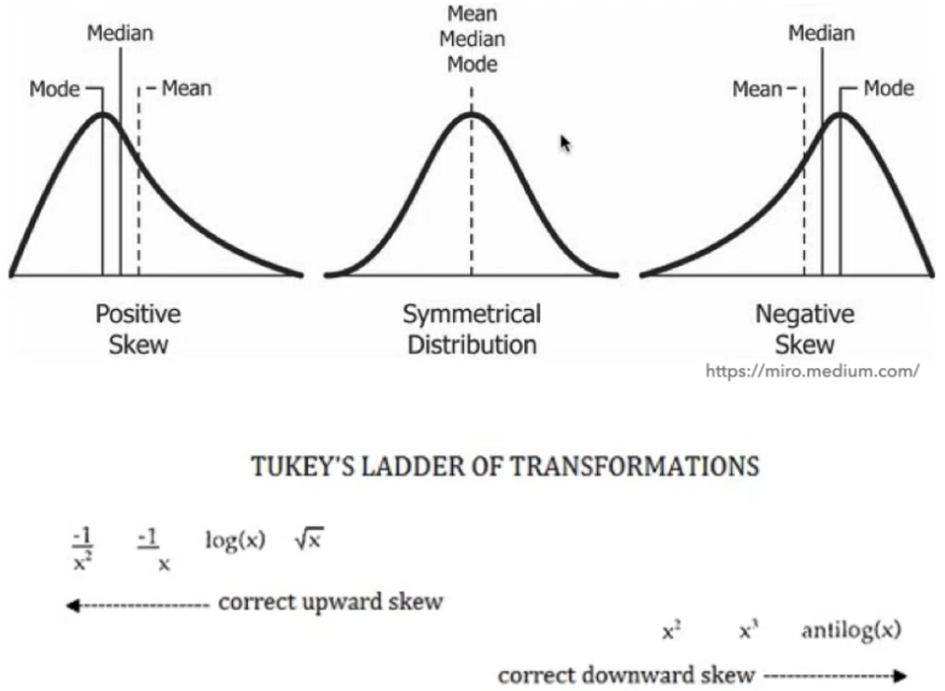
\includegraphics[width=0.6\textwidth]{figtukey}
    \caption{\small{}}
    \label{figtukey}
\end{figure}
\begin{figure}[H]
    \centering
    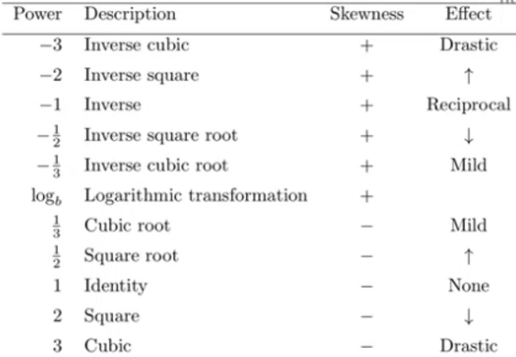
\includegraphics[width=0.6\textwidth]{figtukey2}
    \caption{\small{}}
    \label{figtukey2}
\end{figure}

\subsection{Alternative non parametriche}

Nei casi in cui non si possono usare le trasformazioni, usarle non ha senso o il loro impiego risulta inutile, si ricorre a \textbf{test non parametrici}, che necessitano di assunzioni meno restrittive riguardo la ldistribuzione di probabilità della variabile di interesse nella popolazione dalla quale sono stati estratti i dati, il che rende utili questi metodi quando la distribuzione non è normale.\\
I metodi parametrici, invece, si reggono su assunzioni relative alle distribuzioni; sono quindi parametrici tutti quelli incontrati finora, compresi quelli basati sulla distribuzione $t$.

I metodi non parametrici si basano solitamente sui \textbf{ranghi} dei dati, invece che sui loro valori effettivi. I valori osservati vengono ordinati in ordine crescente e viene registrato il rango di ciascuno, ovvero la posizione rispetto alla lista ordinata (es. primo, secondo). Se l'ipotesi nulla è vera, i diversi ranghi saranno distribuiti circa nello stesso modo nei due gruppi; se invece uno dei due gruppi include la maggior parte delle misure più piccole e l'altro la maggior parte delle più grandi, si potrà pensare che ci siano motivi per rifiutare l'ipotesi nulla.\\
L'uso dei ranghi permette di non formulare assunzioni sulla distribuzione di probabilità delle misure, perché tutte le distribuzioni fanno previsioni simili sui ranghi.\\
I test non parametrici sono particolarmente utili quando si hanno outliers, poiché questi ultimi non influenzano indebitamente i ranghi.

\subsubsection{Test dei segni}

Il test dei segni è un test non parametrico alternativo al $t$ test per un campione o per dati appaiati quando non è soddisfatta l'assunzione di normalità.\\
Il test valuta se la mediana di una popolazione sia uguale ad un valore specificato dall'ipotesi nulla. Le misure che si trovano al di sopra del valore specificato dall'ipotesi nulla vengono classificate ``+'', quelle al di sotto ``-''. Si determina se la frequenza di ``+'' e ``-'' è coerente con quella che si potrebbe trovare per caso. Se l'ipotesi nulla è vera, ci si aspetta che metà delle misure sia situata al di sopra della mediana specificata dall'ipotesi nulla, e che metà sia situata al di sotto, a meno dell'errore di campionamento. È possibile calcolare il P-value usando la distribuzione binomiale. Il test dei segni è un test binomiale in cui il numero delle unità maggiori o minori della mediana specificata dall'ipotesi nulla viene confrontato con quello atteso quando $p = 1/2$.\\
La dimensione campionaria minima necessaria per poter eseguire il test per $\alpha = 0.05$ è $n = 5$.\\
Dunque, si applica la binomiale:
\begin{equation}
    Pr\ [X\ eventi] = \binom{n}{X}\ p^x\ (1-p)^{n-X}
\end{equation}
Il test dei segni ha una potenza molto bassa rispetto al $t$ test per un campione o per dati appaiati, poiché non tiene conto della maggior parte delle informazioni contenute nei dati (es. una misura solo leggermente maggiore del valore della mediana specificato dall'ipotesi nulla o un valore molto più grande vengono conteggiati entrambi come ``+''); nonostante questo, il test è utile perché a volte è impossibile usare altri test.

\subsubsection{Test dei segni per ranghi di Wilcoxon}

Il test dei segni per ranghi di Wilcoxon è un'evoluzione di quello dei segni classico, a differenza del quale conserva le informazioni sui valori assoluti, ovvero tiene conto di quanto ogni valore si discosti dalla mediana ipotizzata; purtroppo, lo fa assumendo che la distribuzione delle misure nella popolazione sia simmetrica attorno alla mediana, e quindi assume che non vi sia asimmetria, il che limita l'utilità del test.\\
Il test ordina per ranghi le differenze assolute (tra ogni dato e la mediana o tra ogni dato e l'altro dato a seconda del tipo di coppia, es. nel caso della guida, la differenza corrisponde a $\delta$, tra il valore birra e quello cellulare), assegna loro il segno (ai positivi ``+'', ai negativi ``-''), calcola il valore assoluto delle differenze, ordina i valori assoluti ed assegna loro i ranghi (primo al valore più alto), somma i ranghi dei + e poi quelli dei - (anche i ranghi ripetuti!), in ultimo, considera il rango più alto (tra i due che risultano dalle due somme?) ($T$) e lo confronta con una statistica di riferimento.\\
???????????????????? (20211206, ca 1:27):
\begin{equation}
    m_T = \frac{n(n+1)}{4}
\end{equation}

Il rango più elevato è il primo, che ha il valore minore.\\
Se due valori della distribuzione sono uguali, questi hanno stesso rango, dunque il numero dei ranghi non sempre coincide con $n$, ma nella somma dei ranghi si deve comunque tenere conto delle ripetizioni, sommando un rango tutte le volte che appare, quindi alla fine i dati rimangono $n$.\\

\subsubsection{Confronto tra due gruppi: test \texorpdfstring{$U$}{Lg} di Mann-Whitney}

Il \textbf{test $U$ di Mann-Whitney}, un test alternativo non parametrico, può essere impiegato al posto del test $t$ per due campioni quando l'assunzione di normalità non è soddisfatta. Il test considera i ranghi delle misure per valutare se le distribuzioni di frequenza di due gruppi siano uguali. Se le distribuzioni dei due gruppi hanno la stessa forma, allora il test si può usare per confrontare le posizioni centrali (mediana o media) nei due gruppi.

\begin{example}[cannibalismo sessuale nei grilli]\label{esgrilli}
    Nella specie \textit{Cyphoderris strepitans} le femmine si accoppiano con maschi che permettono loro di mangiare parte delle proprie ali. Le femmine sono quindi più inclini all'accoppiamento quando sono affamate?\\
    In uno studio, 24 femmine sono state casualmente divise in due gruppi: uno di 11 è stato tenuto a digiuno per almeno 2 giorni, uno di 13 è stato alimentato durante lo stesso intervallo di tempo. Poi, tutte le femmine sono state poste in gabbie separate contenenti un maschio vergine ed è stato registrato il tempo trascorso fino all'accoppiamento (in ore). I dati sono riportati in Tabella \ref{tabgrilli}:
    \begin{table}[H]
        \centering
        \renewcommand\arraystretch{1.2}
        \begin{tabular}{c|c}
        \textbf{Non alimentate} & \textbf{Alimentate}\\ 
        \hline
        1.9 & 1.5\\
        \hline
        2.1 & 1.7\\
        \hline
        3.8 & 2.4\\
        \hline
        9.0 & 3.6\\
        \hline
        9.6 & 5.7\\
        \hline
        13.0 & 22.6\\
        \hline
        14.7 & 22.8\\
        \hline
        17.9 & 39.0\\
        \hline
        21.7 & 54.4\\
        \hline
        29.0 & 72.1\\
        \hline
        72.3 & 73.6\\
        \hline
         & 79.5\\
        \hline
         & 88.9\\
        \hline
        \end{tabular}
        \caption{\small{}}
        \label{tabgrilli}
    \end{table}\noindent
    Le ipotesi sono:
    \begin{itemize}\tightlist
        \item $H_0$: il tempo di attesa fino all'accoppiamento è lo stesso per femmine a digiuno e per femmine alimentate;
        \item $H_A$: il tempo di attesa fino all'accoppiamento differisce tra i due gruppi.
    \end{itemize}
    Il test è a due code. Le distribuzioni di frequenza per i due gruppi sono riportati in Figura \ref{fig13.5-1}:
    \begin{figure}[H]
        \centering
        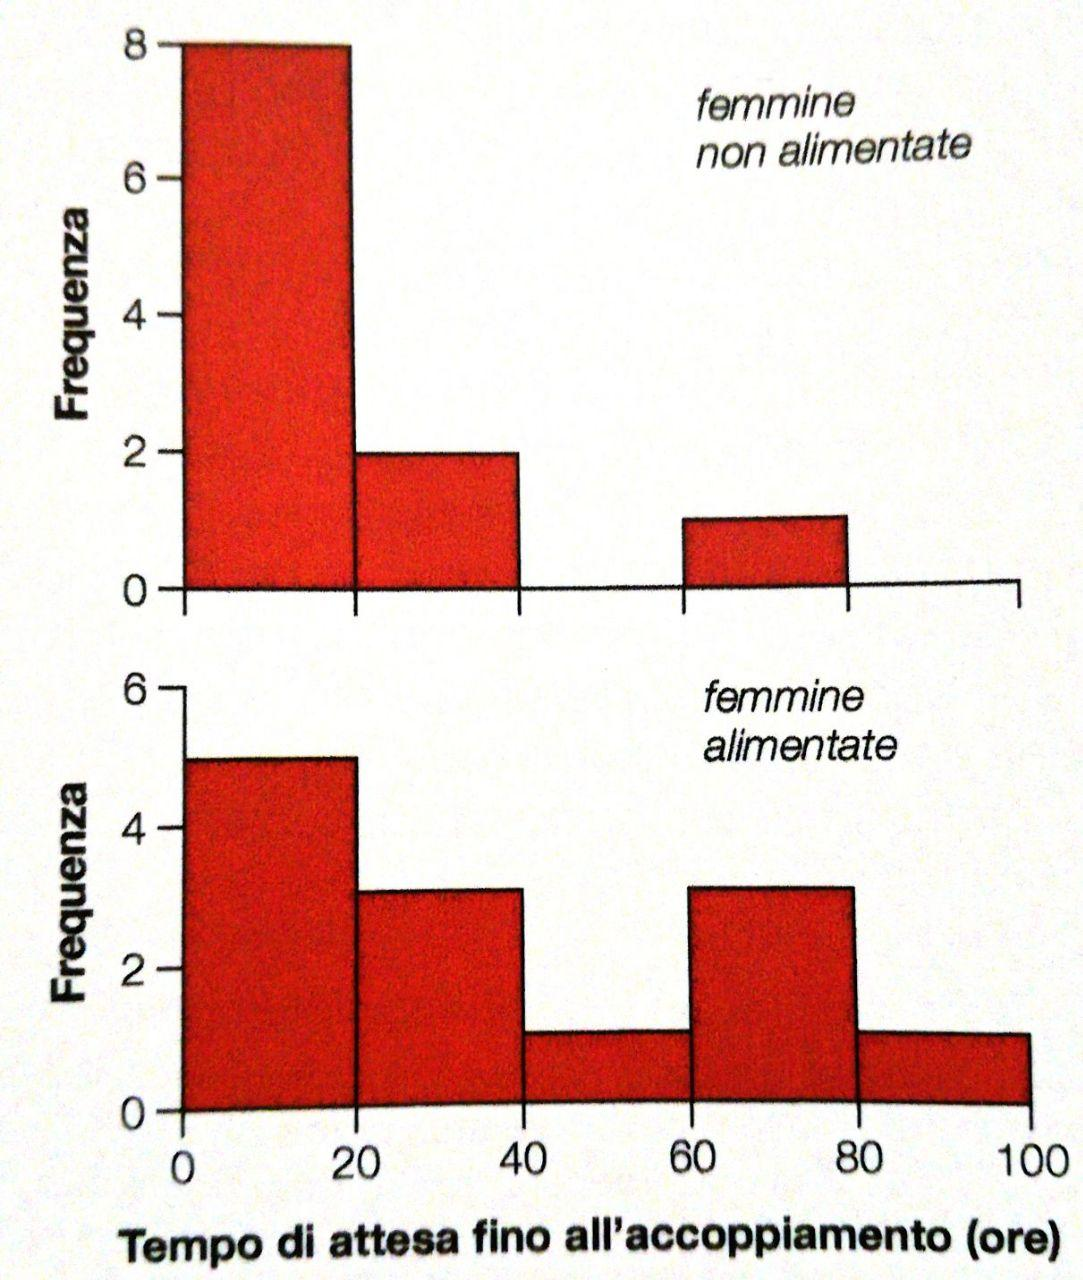
\includegraphics[width=0.6\textwidth]{fig13.5-1}
        \caption{\small{}}
        \label{fig13.5-1}
    \end{figure}
    Nessuno dei due gruppi presenta distribuzione normale, nemmeno dopo una trasformazioni logaritmica. Date le dimensioni ridotte del campione, non si può fare affidamento sul teorema del limite centrale per avere una distribuzione campionaria normale delle medie, quindi non si può impiegare il $t$ test per due campioni.\\
    \begin{figure}[H]
        \centering
        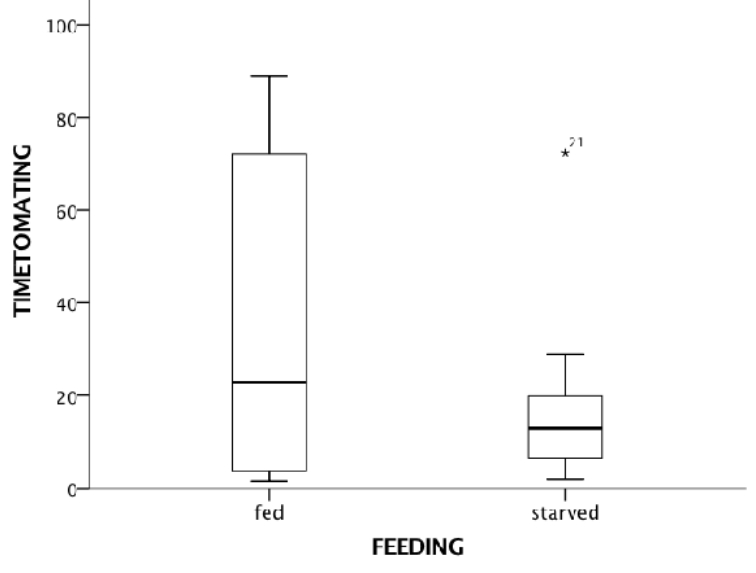
\includegraphics[width=0.4\textwidth]{grilli}
        \caption{\small{}}
        \label{grilli}
    \end{figure}

    Si applica quindi il test U di Mann-Whitney.\\
    Si hanno $n_1 = 11$ femmine non alimentate (gruppo 1) ed $n_2 = 13$ alimentate (gruppo 2).\\
    Per applicare il test U si devono ordinare tutti i valori, in ordine crescente, combinando i dati dei due gruppi, e si deve assegnare un rango a ciascuno di essi. Il rango più elevato, 1, si assegna al valore minore (Tabella \ref{tabgrilli2}):
    \begin{table}[H]
        \centering
        \renewcommand\arraystretch{1.2}
        \begin{tabular}{c|c|c}
        \textbf{Gruppo} & \textbf{Tempo} & \textbf{Rango}\\ 
        \hline
        2 & \color{red}1.5 & \color{red}1\\
        \hline
        2 & \color{red}1.7 & \color{red}2\\
        \hline
        1 & 1.9 & 3\\
        \hline
        1 & 2.1 & 4\\
        \hline
        2 & \color{red}2.4 & \color{red}5\\
        \hline
        2 & \color{red}3.6 & \color{red}6\\
        \hline
        1 & 3.8 & 7\\
        \hline
        2 & \color{red}5.7 & \color{red}8\\
        \hline
        1 & 9.0 & 9\\
        \hline
        1 & 9.6 & 10\\
        \hline
        1 & 13.0 & 11\\
        \hline
        1 & 14.7 & 12\\
        \hline
        1 & 17.9 & 13\\
        \hline
        1 & 21.7 & 14\\
        \hline
        2 & \color{red}22.6 & \color{red}15\\
        \hline
        2 & \color{red}22.8 & \color{red}16\\
        \hline
        1 & 29.0 & 17\\
        \hline
        2 & \color{red}39.0 & \color{red}18\\
        \hline
        2 & \color{red}54.4 & \color{red}19\\
        \hline
        2 & \color{red}72.1 & \color{red}20\\
        \hline
        1 & 72.3 & 21\\
        \hline
        2 & \color{red}73.6 & \color{red}22\\
        \hline
        2 & \color{red}79.5 & \color{red}23\\
        \hline
        2 & \color{red}88.9 & \color{red}24\\
        \hline
        \end{tabular}
        \caption{\small{}}
        \label{tabgrilli2}
    \end{table}\noindent
    Si calcola poi la somma dei ranghi per uno dei due gruppi (più facile usare il gruppo meno numeroso). $R_1 = 121$ è la somma dei ranghi del gruppo 1. Tale valore si usa per calcolare la grandezza $U_1$:
    \begin{equation}
        U_1 = n_1n_2 + \frac{n_1(n_1+1)}{2}-R_1
    \end{equation}
    Che risulta pari a 88, e rappresenta il numero di volte che un valore del campione 1 è minore di un valore del campione 2 se si confrontassero tutte le possibili coppie di punti prelevando in ciascuna coppia un valore da un campione ed un valore dall'altro. Nello stesso modo, $U_2$ risulta pari a 55 (ottenibile anche calcolando $n_1n_2 - U_1$).\\
    Si sceglie il valore di $U$ maggiore, quindi, in questo caso, $U_1$, che diventa la statistica test di riferimento.\\
    Infine, si determina il P-value confrontando il valore di $U$ calcolato con il valore critico della distribuzione nulla per $U$. I valori critici nei casi in cui le dimensioni campionarie sono relativamente piccole sono riportati nella Tavola statistica E (\ref{tavE}). L'ipotesi nulla nulla viene rifiutata se $U$ è maggiore o uguale al valore critico di $U$.\\
    Nell'esempio, con $\alpha = 0.05$, $n_1 = 11$ ed $n_2 = 13$, il valore critico di $U$ è $U_{0.05(2),11,13} = 106$ e, dato che $U$ è pari ad 88, $P>0.05$ e non si può rifiutare l'ipotesi nulla. I dati, quindi, non dimostrano che il tempo di attesa fino all'accoppiamento sia diverso tra i due gruppi.
\end{example}

Il test $U$ funziona bene, soprattutto se associato a permutazione.

\subsubsection{Assunzioni dei test non parametrici}

Le assunzioni dei test non parametrici sono:
\begin{itemize}\tightlist
    \item campioni indipendenti e casuali;
    \item variabili distribuite in modo continuo (assunzione non rigorosa);
    \item simmetria (per test dei segni di Wilcoxon)
    \item stessa forma rispetto alla simmetria (per test $U$);
    \item misure con una scala almeno ordinale (assunzione non rigorosa).
\end{itemize}

\chapter{Disegni sperimentali}

Il classico \textbf{disegno sperimentale} è un esperimento controllato, ovvero in cui si cerca di ottenere che i due o più gruppi osservati differiscano solo per la variabile di interesse. Questo tipo di esperimento si conduce tipicamente in laboratorio.\\
Un \textbf{disegno quasi-sperimentale} è semi-controllato, tipicamente condotto sul campo, in cui alcune condizioni non possono essere controllate; in questi casi, comunque, è necessario tenere ocnto il più possibile di tali condizioni.\\
In uno \textbf{studio osservazionale} non si ha controllo sulle condizioni dei gruppi osservati ma, attraverso dei \textbf{disegni di campionamento} adeguati, è possibile identificare le diverse unità statistiche in modo da avere un range di variazione delle variabili d'interesse.\\
Nella \textbf{discovery science} non si ha nessuna ipotesi specifica di partenza, si studiano i dati, alla ricerca di pattern, a partire dai quali si formulano poi delle ipotesi.\\

Il disegno sperimentale è necessario per:
\begin{itemize}
    \item ridurre la distorsione nella stima e nella verifica degli effetti dei trattamenti;
    \item limitare gli effetti delle variabili di confondimento;
    \item ridurre gli effetti dell'errore di campionamento.
\end{itemize}

In un disegno sperimentale:
\begin{itemize}
    \item si hanno almeno due gruppi (o due variabili, se l'obiettivo è misurare il grado di associazione tra due variabili), uno dei quali è il \textbf{gruppo di controllo}, sul quale si effettuano le stesse misurazioni portate avanti sull'altro (o gli altri), ma che non viene sottoposto al trattamento;
    \item il trattamento si assegna casualmente ai gruppi, per ridurre la distorsione;
    \item si sceglie un $n$ adeguato, per ridurre l'errore di campionamento.
\end{itemize}

\begin{example}[ridurre la trasmissione dell'HIV]\label{eshiv}
    Durante esperimenti in laboratorio, lo spermicida nonoxynol-9 ha manifestato efficacia nel combattere il virus HIV-1. In uno studio successivo, i ricercatori hanno valutato se un gel vaginale contenente lo spermicida fosse riducesse il rischio di contrarre la malattia. Sono stati raccolti dati da 765 prostitute non infette da HIV in 6 ambulatori, in ognuno dei quali è stato assegnato casualmente alle donne un trattamento: con spermicida e senza. Il trattamento dei soggetti era ignoto sia per i soggetti stessi che per i ricercatori. I dati raccolti sono riportati in Tabella \ref{tabhiv}:
    \begin{table}[H]
        \centering
        \renewcommand\arraystretch{1.2}
        \begin{tabular}{c||c|c|c|c}
        \textbf{Ambulatorio} & \textbf{\makecell{n con\\trattamento}} & \textbf{\makecell{n infetti\\con trattamento}} & \textbf{\makecell{n con\\placebo}} & \textbf{\makecell{n infetti\\con placebo}}\\ 
        \hline
        \hline
        Abidjan & 78 & 0 & 84 & 5\\
        \hline
        Bangkok & 26 & 0 & 25 & 0\\
        \hline
        Cotonou & 100 & 12 & 103 & 10\\
        \hline
        Durban & 94 & 42 & 93 & 30\\
        \hline
        Hat Yai 2 & 22 & 0 & 25 & 0\\
        \hline
        Hat Yai 3 & 56 & 5 & 59 & 0\\
        \hline
        \hline
        \textbf{Totali} & 376 & 59 & 389 & 45\\
        \end{tabular}
        \caption{\small{}}
        \label{tabhiv}
    \end{table}\noindent
    Le ipotesi sono:
    \begin{itemize} \tightlist
        \item $H_0$: i soggetti trattati con spermicida e quelli trattati con placebo contraggono il virus allo stesso modo;
        \item $H_A$: i soggetti trattati con spermicida contraggono il virus meno di quelli trattati con placebo.
    \end{itemize}
    Si può calcolare l'odds ratio (+ IC), usare la binomiale, Poisson, o il $\chi^2$.
\end{example}

\section{Riduzione della distorsione}

\subsection{Gruppo di controllo}

Il gruppo di controllo è un gruppo di soggetti trattati come tutti gli altri impiegati nell'esperimento, a eccezione del fatto che non ricevono il trattamento d'interesse.\\
L'impiego del controllo serve per accertarsi che i cambiamenti osservati nei soggetti siano dovuti al trattamento, e non ad altre condizioni, dette confondenti.

\subsection{Randomizzazione}

I trattamenti sono assegnati alle unità in modo casuale. La randomizzazione spezza l'associazione tra possibili variabili di confondimento e la variabile esplicativa, permettendo di valutare la relazione causa-effetto tra variabile esplicativa e variabile risposta. Effettuando correttamente la randomizzazione, la variabilità dovuta alle variabili di confondimento è imputabile esclusivamente al caso, e viene quindi presa automaticamente in considerazione dai metodi classici di inferenza statistica.

\subsection{Cecità}

La cecità (blinding) è il processo per cui si nascondono ai partecipanti le informazioni su quali soggetti ricevono quali trattamenti. Tale processo impedisce ai soggetti e ai ricercatori di modificare il proprio comportamento. In un \textbf{esperimento in singolo cieco}, sono solo i soggetti a non conoscere quale trattamento sia stato loro assegnato, mentre, in un \textbf{esperimento in doppio cieco}, l'informazione è sconosciuta anche ai ricercatori.

\section{Riduzione dell'errore di campionamento}

\subsection{Replicazione}

La replicazione richiede che ogni trattamento venga ripetuto in più unità sperimentali. Gli studi con grandi dimensioni campionarie presentano errori standard più piccoli ed una maggiore probabilità di ottenere una risposta corretta in fase di verifica delle ipotesi.

\subsection{Bilanciamento}

Il disegno di uno studio si dice bilanciato se tutti i trattamenti hanno la stessa dimensione campionaria. 

\subsection{Raggruppamento in blocchi}

Il raggruppamento in blocchi serve per tenere conto della variabilità non dovuta al trattamento. Le unità sperimentali vengono suddivise in gruppi, detti \textbf{blocchi} o strati, all'interno dei quali i singoli elementi condividono le condizioni generali dell'ambiente sperimentale (escluso il trattamento). Nei blocchi i trattamenti vengono assegnati casualmente ai singoli, e le differenze tra trattamenti vengono valutate solo entro i blocchi, eliminando molta della variabilità che deriva dalle differenze tra essi.\\
I disegni a blocchi randomizzati si usano molto in ecologia.\\
Il ragruppamento in blocchi è un metodo dibattuto.

\section{Disegno sperimentale fattoriale}

Un \textbf{disegno sperimentale fattoriale} prevede che si analizzino più fattori contemporaneamente (es. influenza di un trattamento su due distinte linee genetiche e sul sesso degli individui), ed eventualmente anche le relazioni tra i due o più fattori che si analizzano (es. c'è differenza a livello genetico, ma l'entità della differenza varia a seconda del sesso).
\begin{example}[sopravvivenza dei girini]\label{esgirini}
    Uno studio ha indagato se la presenza di una piccola dose di un pesticida influenzasse la sopravvivenza dei girini di Rana Toro, per valutare se l'effetto di tale pesticida dipendesse dalla presenza/assenza di una salamandra predatrice autoctona. L'esperimento è stato portato avanti in vasche con 10 girini ciascuna, e le quattro possibili combinazioni di due trattamenti con pesticida (con o senza) e due trattamenti con predatori (presenti o assenti) sono state assegnate casualmente alle vasche. Per ciascuna delle 4 combinazioni sono state previste 4 repliche (quindi 16 vasche totali). Gli effetti sulla sopravvivenza dei girini sono presentati nel diagramma in Figura \ref{fig14.5-1}:\\
    \begin{figure}[H]
        \centering
        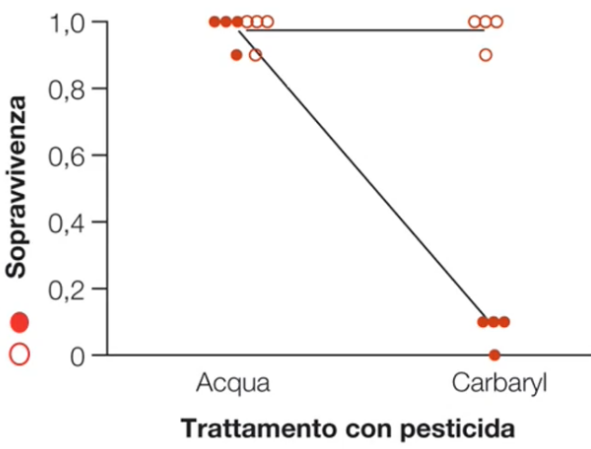
\includegraphics[width=0.5\textwidth]{fig14.5-1}
        \caption{\small{}}
        \label{fig14.5-1}
    \end{figure}

    La variabile risposta è la sopravvivenza dei girini, mentre le variabili che generano una variazione nella variabile risposta sono due, pesticida e predatore, ciascuno con due livelli (con/senza e presente/assente).\\
    In questo caso non si potrebbe utilizzare il test del $\chi^2$, poiché la variabile risposta non è nominale, ma continua.\\
    Si nota come, in assenza di predatore, non esiste evidenza sperimentale che supporti l'ipotesi che il pesticida da solo condizioni la sopravvivenza dei girini. In presenza del predatore, questo non ha effetto sulla sopravvivenza dei girini, nel caso in cui il pesticida è assente. C'è dunque un'interazione tra i due fattori.
\end{example}

\section{Impossibilità di condurre esperimenti}

Quando non è possibile condurre studi sperimentali ci si limita a studi osservazionali, molto importanti poiché permettono di identificare pattern e formulare ipotesi. L'unica tecnica volta alla riduzione della distorsione che non si può utilizzare negli studi osservazionali è la randomizzazione, poiché il ricercatore non può assegnare i trattamenti ai soggetti, ma solo osservarli allo stato naturale.\\
Per limitare gli effetti di variabili di confondimento negli studi osservazionali si usano appaiamento e aggiustamento.\\
Nell'\textbf{appaiamento}, ogni individuo che presenta la condizione d'interesse si associa ad uno che non la presenta, ma che presenta quanto più possibile tutte le altre caratteristiche del primo. In qusto modo, comunque, si possono controllare solo le variabili di confondimento misurate esplicitamente. L'appaiamento riduce anche l'errore di campionamento, raggruppando i soggetti in coppie di individui simili, analogamente al raggruppamento in blocchi negli studi sperimentali.\\
L'\textbf{aggiustamento} prevede invece di utilizzare metodi statistici, come l'analisi della covarianza, per correggere le differenze tra gruppi di trattamento e gruppi di controllo dovute a potenziali variabili di confondimento.

\section{Dimensione di un campione}

I comitati etici per gli studi sull'uomo e per la sperimentazione animale impongono ai ricercatori di giustificare le dimensioni campionarie per gli esperimenti proposti. Tale decisione viene presa considerando la precisione nella stima dell'effetto di un trattamento e la potenza predeterminata nella verifica dell'ipotesi nulla secondo cui il trattamento non ha effetto.\\
Le tecniche impiegate negli studi pianificati per confrontare le medie di due gruppi sono riportate di seguito.

\subsection{Pianificare la precisione}

Per ottenere la precisione desiderata si deve scegliere una dimensione campionaria che fornisca un intervallo di confidenza con una certa ampiezza.\\
Nel caso in cui si debba pianificare uno studio per confrontare le medie tra due trattamenti, si assume che la media incognita della variabile risposta della popolazione sia $\mu_1$, nel gruppo che ha ricevuto il trattamento di interesse e $\mu_2$ nel gruppo controllo. Una volta ottenuti i risultati si calcolano le medie campionarie $\overline{Y}_1$ e $\overline{Y}_2$ e si usano per valutare l'intervallo di confidenza al 95\% per $\mu_1 - \mu_2$, la differenza tra media nella popolazione con trattamento e media nella popolazione di controllo. Assumendo che le dimensioni campionarie per entrambi i trattamenti abbiano lo stesso valore ($n$), si assume anche le due popolazioni abbiano una distribuzione normale della variabile studiata e stessa deviazione standard ($\sigma$). In questo caso, l'intervallo di confidenza al 95\% per $\mu_1 - \mu_2$ è dato da:
\begin{equation}
    \overline{Y}_1 - \overline{Y}_2 \pm incertezza
\end{equation}
In cui ``incertezza'' e metà dell'ampiezza dell'intervallo di confidenza. per pianificare lo studio in modo da ottenere la precisione desiderata si deve decidere in anticipo l'incertezza che si può tollerare. Una volta presa questa decisione, la dimensione campionaria necessaria in ciascun gruppo è circa:
\begin{equation}
    n = 8 \left(\frac{\sigma}{incertezza}\right)^2   
\end{equation}
Formula dedotta dalla regola dei 2ES (\ref{????????}). Secondo questa relazione, è necessaria una dimensione campionaria Maggiore quando la deviazione standard nei gruppi e grande anziché piccola. Inoltre per ottenere un'elevata precisione, e quindi una ridotta incertezza, è necessaria una dimensione campionaria grande.\\
Un problema rilevante consiste nel fatto che parametri come la deviazione standard non sono noti; generalmente, questi si stabiliscono sulla base di studi pilota.\\
La Figura \ref{fig14.7-1} mostra la precisione attesa dell'intervallo di confidenza al 95\% della differenza tra le medie di due trattamenti in funzione dela dimensione compionaria $n$ in ciascun trattamento, relativamente ad un esempio.
\begin{figure}[H]
    \centering
    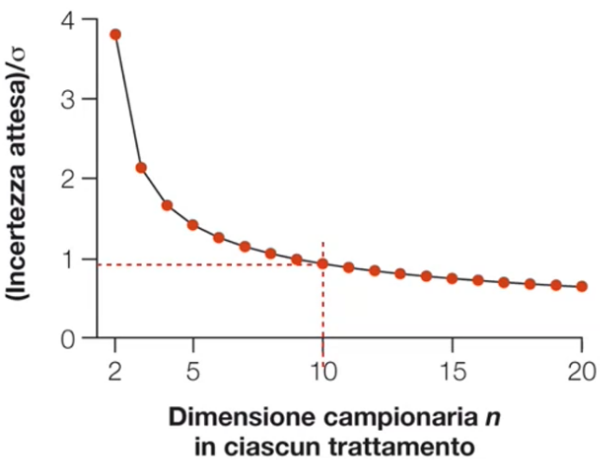
\includegraphics[width=0.5\textwidth]{fig14.7-1}
    \caption{\small{}}
    \label{fig14.7-1}
\end{figure}
Sarebbe auspicabile rimanere sotto un'incertezza minore di 1. Grafici di questo tipo aiutano anche a rendersi conto di quanto si guadagnerebbe in termini di incertezza con un aumento della dimensione campionaria.\\

\subsection{Pianificare la potenza}

L'\textbf{effect size} è la dimensione dell'effetto che si vuole essere in grado di rilevare, al della quale è irrilevante che l'effetto ci sia o meno.\\
Più piccole sono le differenze che si vuole poter distinguere, maggiore deve essere la potenza dello strumento che si utilizza. Per fare ciò si aumentano le repliche e si bilanciano i gruppi.\\
Per determinare l'$n$ adeguato al rilevamento di differenze di una voluta entità si definiscono:
\begin{itemize}\tightlist
    \item ipotesi nulla;
    \item test statistico che si usa per verificare le differenze che si vogliono rilevare;
    \item dimensione dell'effetto che si vuole essere in grado di rilevare;
    \item livelli di rischio che si accettano in termini di errori del I e II tipo.
\end{itemize}

La \textbf{potenza} è pari a:
\begin{equation}
    potenza = 1-\beta
\end{equation}
In cui $\beta$ è l'errore del II tipo (non rifiutare ipotesi nulla quando si dovrebbe).\\
Una potenza convenzionalmente auspicabile è 0.8.\\

Nel confronto tra due medie, quando l'ipotesi nulla vuole che non ci sia differenza e l'ipotesi alternativa vuole che ci sia, se l'obiettivo è una potenza di 0.80 e si assume il livello di significatività $\alpha = 0.05$, un'approssimazione della dimensione campionaria necessaria in ciascuno dei due gruppi è:
\begin{equation}
    n = 16\left(\frac{\sigma}{D}\right)^2
\end{equation}
In cui $D$ è il valore minimo della differenza tra medie che si è interessati ad evidenziare (effect size). La formula assume che le due popolazioni abbiano una distribuzione normale, con la stessa deviaizone standard ($\sigma$).\\

Quando si ottiene un risultato non significativo, una possibilità è che il test usato potrebbe non essere stato abbastanza potente (in relazione all'entità delle differenze che si volevano rilevare).\\

Il calcolo della potenza di un test dato un $n$ è complicato, e varia tra test e disegni sperimentali.\\
Sono disponibili software (es. G-Power, powerandsamplesize.com) in grado di calcolare la potenza che il proprio disegno sperimentale permette di raggiungere (in base alla quale si calcolerà la dimensione campionaria) o viceversa.\\

\subsubsection{Per il \texorpdfstring{$t$}{Lg} test}

Per il $t$ test esistono delle tabelle di valori e:
\begin{itemize}\tightlist
    \item si definiscono l'ipotesi nulla e se l'ipotesi alternativa è ad una o due code (perché in base a questo si definisce $\alpha$);
    \item si stima l'effect size come la differenza tra le due medie che si vuole rilevare;
    \item si stima la variabilità come la deviazione standard (s) di quella variabile;
    \item si calcola l'effect size standardizzato (E/s, con E = effect size);
    \item si definiscono $\alpha$ e $\beta$.
\end{itemize}

\begin{figure}[H]
    \centering
    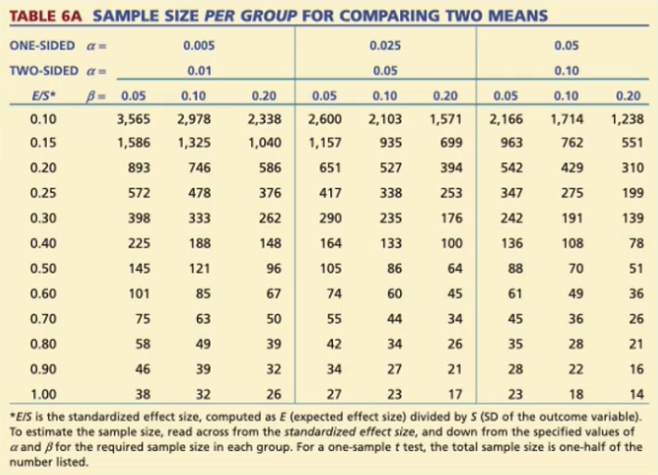
\includegraphics[width=0.6\textwidth]{samplesizet}
    \caption{\small{}}
    \label{samplesizet}
\end{figure}

\subsection{Pianificare per compensare la perdita di dati}

Le commissioni ritengono solitamente accettabile l'utilizzo di un $n$ leggermente più elevato che possa compensare eventuali perdite di dati (es. individui che rispondono in maniera anomala o muoiono, campioni che vanno persi).

\chapter{Confronto tra le medie di più di due gruppi}\footnote{In questo capitolo si affronta il metodo ANOVA ``a una via'', che confronta le medie di più gruppi che differiscono per un solo fattore, una sola variabile esplicativa.}

\section{Analisi della varianza}

L'analisi della varianza (ANOVA) è il metodo conosciuto più potente per valutare simultaneamente se le medie di $k$ gruppi siano uguali. In sostanza, l'ANOVA verifica se individui appartenenti a differenti gruppi siano in media più diversi rispetto ad individui appartenenti allo stesso gruppo.\\
Basandosi sulla varianza, l'ANOVA è un test parametrico.

\begin{example}[effeto della luce sul ritmo circadiano]\label{esluce}
    Il disturbo del jet lag si supera quando l'alternarsi della luce e del buio percepito dagli occhi del nuovo fuso orario sincronizza di nuovo e gradualmente l'orologio circadiano interno, che aveva subito uno sfasamento.\\
    Uno studio suggerisce che l'orologio circadiano umano possa essere sincronizzato di nuovo anche con l'esposizione della superficie posteriore del ginocchio alla luce. Alcuni aspetti del disegno sperimentale di tale studio sono stati messi in discussione.\\
    I dati riportati in Tabella \ref{tabluce} provengono da un secondo studio in cui è stato riesaminato il fenomeno ed in cui il ritmo circadiano è stato misurato valutando il ciclo giornaliero di produzione di melatonina in 22 soggetti assegnati casualmente a uno di tre diversi trattamenti. I soggetti sono stati svegliati dal sonno e sottoposti a un singolo episodio di tre ore di illuminazione intensa applicata soltanto agli occhi, soltanto alle ginocchia, né agli occhi né alle ginocchia (gruppo di controllo).\\
    \begin{table}[H]
        \centering
        \renewcommand\arraystretch{1.2}
        \begin{tabular}{c||c|c|c|c}
        \textbf{Trattamento} & \textbf{Dati (h)} & \textbf{$\overline{Y}$} & \textbf{s} & \textbf{n}\\ 
        \hline
        \hline
        Controllo & 0.53, 0.36, 0.20, -0.37, -0.64, -0.68, -1.27 & -0.3088 & 0.6176 & 8\\
        \hline
        Ginocchia & 0.73, 0.31, 0.03, -0.29, -0.56, -0.96, -1.61 & -0.3357 & 0.7908 & 7\\
        \hline
        Occhi & -0.78, -0.86, -1.35, -1.48, -1.52, -2.04, -2.83 & -1.5514 & 0.7063 & 7\\
        \hline
        \end{tabular}
        \caption{\small{}}
        \label{tabluce}
    \end{table}\noindent
    Gli effetti del trattamento sono stati misurati due giorni dopo valutando l'entità dello sfasamento nel ciclo giornaliero di produzione di melatonina di ciascun soggetto. I risultati sono riportati in Figura \ref{fig15.1-1}:
    \begin{figure}[H]
        \centering
        \includegraphics[width=0.5\textwidth]{fig15.1-1}
        \caption{\small{}}
        \label{fig15.1-1}
    \end{figure}
    Una misura negativa indica un ritardo nella produzione di melatonina, che è l'effetto previsto del trattamento luminoso, mentre una misura positiva indica un anticipo.\\
    L'ipotesi nula dell'ANOVA è che le medie delle popolazioni, $\mu_i$, siano uguali per tutti i trattamenti. Se l'ipotesi nulla è vera, le differenze tra le medie dei campioni $\overline{Y}_i$ sono dovute solo a errori di campionamento. L'ipotesi alternativa implica invece che lo sfasamento medio non sia uguale nelle tre popolaszioni; dunque, le ipotesi sono:
    \begin{itemize}
        \item $H_0$: $\mu_1 = \mu_2 = \mu_3$;
        \item $H_A$: almeno una delle medie è diversa dalle altre.
    \end{itemize}
    Anche nel caso in cui fosse vera l'ipotesi nulla, quindi se le popolazioni campionarie avessero medie uguali, le medie campionarie calcolate in base ai dati sarebbero diverse tra loro per effetto del caso. Il compito dell'ANOVA e determinare se la variazione tra le medie campionarie dei gruppi sia maggiore di quella attesa per effetto del caso, il che indicherebbe che almeno una delle medie delle popolazioni è diversa dalle altre e che l'ipotesi nulla deve essere rifiutata.\\
    L'ANOVA permette di ottenere tale risultato confrontando due fonti di variabilità nei dati, illustrate in Figura 15.1-2 per i dati sul ritmo circadiano:
    \begin{figure}[H]
        \centering
        \includegraphics[width=0.7\textwidth]{fig15.1-2}
        \caption{\small{}}
        \label{fig15.1-2}
    \end{figure}
    I dati sono stati dispersi orizzontalmente per consentire di vederli meglio. La prima parte della figura presenta tutta la variabilità nei dati. Un segmento verticale rappresenta lo scarto totale di ogni dato dalla media generale di tutti i dati. Se si elevassero al quadrato tali scarti e si calcolasse la loro media, si otterrebbe la varianza campionaria di tutti i dati considerati assieme.\\
\end{example}

L'ANOVA suddivide lo scarto totale di ogni osservazione in due parti, che rappresentano le due fonti di variabilità nei dati: 
    \begin{itemize}\tightlist
        \item lo scarto di ogni osservazione dalla media del suo gruppo, detto \textbf{errore}, o residuo (grafico a destra);
        \item lo scarto della media del gruppo a cui l'osservazione appartiene rispetto alla media generale (grafico centrale).
    \end{itemize}
Si possono quindi ottenere due tipi di varianza:
    \begin{itemize}\tightlist
        \item \textbf{media dei quadrati entro gruppi} (o varianza entro gruppi o media dei quadrati degli errori o varianza campionaria comune), che rappresenta la variabilità tra gli individui appartenenti allo stesso gruppo, e si ottiene elevando al quadrato gli errori e calcolando la media dei risultati (le barre verticali nel terzo grafico sono gli scarti di ciascuna unità rispetto alla media del proprio gruppo);
        \item \textbf{media dei quadrati tra gruppi}, una specie di media dei quadrati degli scarti nel grafico centrale, che rappresenta la variabilità tra individui appartenenti a differenti gruppi (le barre verticali nel secondo grafico sono tutte uguali entro uno stesso gruppo, e rappresentano lo scarto medio dalla media totale di ciascun gruppo, ripetuto il numero di unità in ogni gruppo, come per fare una specie di media ponderata).
    \end{itemize}
Se l'ipotesi nulla fosse vera e le medie delle popolazioni nei gruppi fossero 
quindi uguali, le due medie dei quadrati dovrebbero essere circa uguali, e la variabilità tra individui appartenenti a differenti gruppi non sarebbe diversa da quella tra individui appartenenti allo stesso gruppo, eccezion fatta per l'effetto del caso. Se invece la media dei quadrati tra gruppi è significativamente maggiore della media dei quadrati degli errori, esistono differenze reali tra le medie delle popolazioni; il risultato finale dell'ANOVA è un testo che confronta queste due medie di quadrati.

\subsection{Calcolo delle medie dei quadrati}

\subsubsection{Media dei quadrati entro gruppi}

La media dei quadrati entro gruppi ($MS_{entro}$, o $MS_{errore}$, Mean Square dell'errore, Quadrato Medio, QM in italiano) misura la varianza nei gruppi.\\
L'ANOVA assume che la varianza ($\sigma^2$) sia la stessa in ogni popolazione. La migliore stima di tale varianza entro gruppi è la varianza campionaria comune, come nel $t$ test per due campioni (\ref{??????}).\\
Nell'ANOVA:
\begin{equation}
    MS_{entro} = \frac{\sum{s_i^2(n_i-1)}}{N-k}
\end{equation}
In cui:
\begin{itemize}\tightlist
    \item $s_i$ sono le deviazioni standard campionarie ottenute da ciascun gruppo;
    \item $n_i$ sono le dimensioni campionarie dei gruppi;
    \item $n_i - 1$ è il numero di gradi di libertà del gruppo $i$-esimo;
    \item il denominatore è la somma dei gradi di libertà per i diversi gruppi ($\sum{n_i - 1} = N-k$);
    \item $N$ è il numero totale delle osservazioni nell'insieme dei gruppi ($\sum{n_i = N}$);
    \item il numeratore è la Sum of Squares (SS), la somma di tutti i quadrati degli scarti, corrisponde alla devianza.
\end{itemize}

\subsubsection{Media dei quadrati tra gruppi}

La media dei quadrati tra gruppi ($MS_{tra}$, o $MS_{gruppi}$) si calcola sulla abse degli scarti delle medie campionarie di ciascun gruppo ($\overline{Y}_i$) rispetto alla media generale di tutte le misure ($\overline{Y}$):
\begin{equation}
    MS_{tra} = \frac{\sum{n_i(\overline{Y}_i-\overline{Y})^2}}{k-1}
\end{equation}
In cui:
\begin{itemize}\tightlist
    \item $k$ è il numero totale di gruppi;
    \item il denominatore, $k-1$, è il numero di gradi di libertà per i gruppi;
    \item la media generale $\overline{Y}$ è la media di tutti i dati di tutti i gruppi nel loro insieme, che non è uguale alla media delle medie campionarie di ciascun gruppo se la dimensione campionaria non è la stessa in ogni gruppo, e si calcola con la formula:
    \begin{equation}
        \overline{Y} = \frac{\sum{n_i\ \overline{Y}_i}}{N}
    \end{equation}
    che equivale a sommare tutte le misure provenienti da tutti i gruppi e dividere le somma ottenuta per il numero totale di osservazioni.
\end{itemize}

\subsection{Rapporto tra varianze}

Assumendo vera l'ipotesi nulla che le medie delle popolazioni di tutti i gruppi sono uguali, la variabilità tra gli individui appartenenti a diversi gruppi ($MS_{tra}$) dovrebbe essere uguale alla varianza tra gli individui appartenenti allo stesso gruppo ($MS_{entro}$). Nell'ANOVA si valuta un'eventuale differenza tra le due, calcolando il \textbf{rapporto tra varianze} ($F$):
\begin{equation}
    F = \frac{MS_{tra}}{MS_{entro}}
\end{equation}
che è la statistica test dell'ANOVA. Sotto l'ipotesi nulla, F è vicino ad 1, mentre se l'ipotesi nulla è falsa, F è maggiore di 1.\\
Per calcolare il P-value è necessaria la distribuzione campionaria di $F$ sotto l'ipotesi nulla, che è la distribuzione $F$, che ha una coppia di gradi di libertà, uno per il numeratore ed uno per il denominatore del rapporto (rispettivamente, $k-1$ e $N-k$). Il numero di gradi di libertà del numeratore viene presentato per primo quando si specifica la distribuzione $F$.\\
La Figura \ref{fig15.1-3} illustra la distribuzione $F$ dell'esempio sul jet lag (\ref{esluce}), che si estende da 0 a + infinito, con 2 e 19 gradi di libertà (da calcolare sulla base dei dati dell'esempio):\\
\begin{figure}[H]
    \centering
    \includegraphics[width=0.5\textwidth]{fig15.1-3}
    \caption{\small{}}
    \label{fig15.1-3}
\end{figure}

Se l'ipotesi nulla fosse falsa, $MS_{tra}$ sarebbe maggiore di $MS_{entro}$, ed il rapporto $F$ si troverebbe nella coda destra della distribuzione. Rapporti minori di 1 potrebbero presentarsi solo per effetto del caso.\\
Il valore critico corrispondente all'area di 0.05 nella coda destra della distribuzione ($F_{0.05(1),dfnum,dfden}$, (1) perché solo coda destra) si trova nella Tavola statistica D (\ref{tavD}).\\
Il valore critico per l'esempio è $F_{0.05(1),2,19} = 3.52$, quindi l'area sottesa dalla curva a destra di 3.52 è pari a 0.05. Dato che, nell'esempio, il valore osservato di $F$ (7.29) è maggiore di 3.52, esso si trova a destra, oltre il valore critico, quindi $P<0.05$ e si rifiuta l'ipotesi nulla.

\subsection{Valore \texorpdfstring{$R^2$}{Lg}}

I nominatori delle formule delle medie dei quadrati sono Sum of Squares, ovvero devianze. Le devianze hanno una proprietà additiva, quindi la devianza totale corrisponde alla somma della devianza tra gruppi e di quella entro gruppi:
\begin{equation}
    SS_{totale} = SS_{tra}+SS_{entro}
\end{equation}
Il \textbf{valore $R^2$} è usato nell'ANOVA per riassumere il contributo delle differenze tra gruppi alla variabilità nei dati, ed è la porzione della variabilità dovuta ai gruppi/raggruppamenti, espressa come frazione del totale:
\begin{equation}
    R^2 = \frac{SS_{tra}}{SS_{entro}}
\end{equation}
$R^2$ può assumere valori da 0 ad 1:
\begin{itemize}\tightlist
    \item quando è prossimo a 0, le medie dei gruppi sono tutte molto simili, e la maggior parte della variabilità sussiste all'interno dei gruppi. In questi casi, quindi, la variabile esplicativa che definisce i gruppi spiega molto poco la variabilità di $Y$;
    \item quando è prossimo ad 1, resta poca variazione in $Y$ dopo che si è tenuto conto delle diverse medie dei gruppi, quindi la variabile esplicativa spiega la maggior parte della variabilità di $Y$.
\end{itemize}
Nell'esempio, $R^2 = 0.43$, quindi il 43\% della somma dei quadrati totale nel valore dello sfasamento è spiegato dadifferenze tra individui sottoposti a diversi trattamenti luminosi. Il diverso trattamento non spiega il restante 57\% della variabilità tra individui, che è semplicemente ``errore''.

\subsection{Assunzioni dell'ANOVA}

Le assunzioni dell'ANOVA sono uguali a quelle del $t$ test per due campioni, ma devono essere vere per tutti i $k$ gruppi:
\begin{itemize}\tightlist
    \item le misure in ogni gruppo sono un campione casuale estratto dalla corrispondente popolazione;
    \item la variabile è distribuita normalmentein ciascuna delle $k$ popolazioni;
    \item la variabile è la stessa nelle $k$ popolazioni;
    \item le varianze nella risposta sono comparabili.
\end{itemize}
Esistono delle formulazioni modificate per calcolare le varianze che resistono alla violazione dell'omogeneità delle varianze.\\

L'ANOVA è robusta rispetto alle deviazioni dall'assunzione di normalità, soprattutto per grandi dimensioni campionarie. Tale robustezza deriva da una proprietà delle medie campionarie che è descritta dal teorema del limite centrale: entro ogni gruppo la distribuzione campionaria delle medie è approssimativamente normale quando la dimensione del campione è grande, anche se la variabile stessa non ha distribuzione normale.\\
L'ANOVA è robusta anche rispetto agli scostamenti dall'assunzione di uguale varianza nelle $k$ popolazioni, ma solo se i campioni hanno tutti circa la stessa dimensione.\\

Se i dati non sono conformi alle assunzioni dell'ANOVA, essi possono essere trasformati mediante tutte le trasformazioni viste nel capitolo \ref{?????}.

\section{Alternative non parametriche all'ANOVA: test di Kruskal-Wallis}

Se l'assunzione di normalità dell'ANOVA non è soddisfatta e le trasformazioni non funzionano, un'alternativa non parametrica all'ANOVA ad un fattore è il test di Kruskal-Wallis, o analisi della varianza basata sui ranghi, basato sui ranghi, equivalente del test $U$ di Mann-Whitney quando i gruppi sono più di due; le assunzioni di partenza sono infatti le stesse, anche se applicate a più di due gruppi:
\begin{itemize}\tightlist
    \item i campioni di tutti i gruppi sono casuali, estratti dalle corrispondenti popolazioni;
    \item la distribuzione della variabile deve avere la stessa forma in ogni popolazione.
\end{itemize}
Il test prevede di:
\begin{itemize}\tightlist
    \item i dati considerati nel loro insieme vengono ordinati in modo crescente;
    \item si assegna loro un rango;
    \item la somma dei ranghi in ciascun gruppo, $R_i$, viene usata per calcolare la statistica test del test, $H$:
    \begin{equation}
        H = \frac{12}{N(N+1)}\sum{\frac{R_i^2}{N_i}}-3(N+1)
    \end{equation}
    In cui:
    \begin{itemize}\tightlist
        \item $N$ è la dimensione campionaria totale;
        \item $R_i$ è la somma dei ranghi per il gruppo $i$.
    \end{itemize}
    \item si confronta l'H ottenuta con quella attesa sotto l'ipotesi nulla.
\end{itemize}
SOtto l'ipotesi nulla di nessuna differenza tra le popolazioni, la distribuzione campionaria di $H$ è approssimativamente quella del $\chi^2$ con $k-1$ gradi di libertà, in cui $k$ è il numero di gruppi.\\
L'ipotesi nulla viene rifiutata se H è superiore o pari al valore critico ottenuto dalla distribuzione $\chi^2$ appropriata, $\chi^2_{k-1,\alpha(1)}$.\\
Il test di Kruskal-Wallis ha una potenza limitata quando le dimensioni campionarie sono molto piccole. Con dimensioni campionarie adeguate, il test ha circa la stessa potenza dell'ANOVA.

\section{Confronti pianificati e non pianificati}

In alcuni studi, i risultati dell'ANOVA non bastano, ma si vuole sapere anche, ad esempio, quali medie siano diverse, o quale sia l'entità delle differenze riscontrate. Per determinare questi due aspetti sono disponibili due approcci: i confronti pianificati e quelli non pianificati.\\
Un \textbf{confronto pianificato} è un confronto tra medie ritenute d'interesse durante il disegno dello studio, prima della raccolta dei dati, e deve avere una giustificazione valida a priori (es. previsione suggerita da studi precedenti). Per ridurre al minimo gli errori di tipo I, è permesso solo un numero limitato di confronti pianificati.\\
Un \textbf{confronto non pianificato} è uno dei confronti multipli possibili tra tutte le coppie di medie, svolti per identificare a posteriori le medie diverse.

\subsection{Confronti pianificati}

Riprendendo l'esempio \ref{esluce}, l'esperimento si proponeva principalmente di confrontare lo sfasamento medio della produzione di melatonina tra il gruppo sottoposto a trattamento luminoso alle ginocchia ed il gruppo di controllo. Poiché l'esperimento è stato costruito attorno a tale confronto, si possono usare i metodi del confronto pianificato per capire quanto sia grande la differenza tra i due gruppi e se tale differenza sia statisticamente significativa.\\
Il metodo da utilizzare è quasi lo stesso usato nel confronto tra due campioni basato sulla distribuzione $t$, solo che l'errore standard si calcola in modo diverso, usando la varianza campionaria comune (la media dei quadrati degli errori) basata su tutti i $k$ gruppi (ed i corrispondenti gradi di libertà dell'errore), invece di quella basata solo sui due gruppi che vengono confrontati:
\begin{equation}
    ES_{\overline{Y}_i-\overline{Y}_j} = \sqrt{MS_{entro}\ (\frac{1}{n_i}-\frac{1}{n_j})}
\end{equation}
Così aumentano precisione e potenza. L'errore standard per l'ANOVA è sempre più piccolo o al massimo uguale rispetto a quello calcolato per un $t$ test, quindi il metodo è più potente.\\
Il metodo dei confronti pianificati assume, come l'ANOVA, che la varianza sia la stessain tutti i gruppi.\\
A partire dall'errore standard si possono calcolare gli intervalli di confidenza.

\subsection{Confronti non pianificati}

I confronti non pianificati richiedono aggiustamenti delle formule per impedire l'aumento di falsi positivi (errori del tipo I) tipico dei test multipli.\\
Il tipo più comune di confronto non pianificato è valutare tutte le coppie di medie per trovare quali gruppi sono diversi dagli altri. Il \textbf{test di Tukey-Kramer} è la procedura più usata in questi casi; il test assume che sia già stata eseguita un'ANOVA e che l'ipotesi nulla sia stata rifiutata.

\begin{example}[wood wide web]\label{eswww}
    In uno studio è stato misurato il flusso di C tra piantine di betulla e di douglasia ed è stato valutato se la quantità di C che passava nell'unità di tempo dipendesse dall'ombra sulle piante, poiché gli alberi in ombra potrebbero estrarre più C attraverso le micorrize rispetto a quelli al sole. Per ciascuno dei tre trattamenti con diversi livelli d'ombra sono state piantate 5 coppie di piante di betulla e douglasia, che sono state fatte crescere per un anno. Poi ogni piantina di betulla è stata chiusa per 2 h in un sacco sigillato con immissione di $CO_2$ con $^{13}C$, invece del normale $^{12}C$; stesso trattamento per le douglasie, ma con $^{14}C$. Le quantità dei due isotopi presenti nelle piantine sono state misurate 9 giorni dopo. Avendo usato diversi isotopi, si è potuta calcolare la quantità di C trasferita da ciascuna pianta all'altra della coppia d'appartenenza. La maggior parte del trasferimento si è avuto dalla betulla alla douglasia. Alcuni dati sono riportati in Tabella \ref{tabwww}:
    \begin{table}[H]
        \centering
        \renewcommand\arraystretch{1.2}
        \begin{tabular}{c||c|c|c}
        \textbf{Ombra} & \textbf{\makecell{Media\\campionaria\\$\overline{Y}_i$ (mg)}} & \textbf{\makecell{Deviazione\\standard\\campionaria ($s_i$)}} & \textbf{$n_i$}\\ 
        \hline
        \hline
        completa & 18.33 & 6.98 & 5\\
        \hline
        parziale & 8.29 & 4.76 & 5\\
        \hline
        nessuna & 5.21 & 3.00 & 5\\
        \hline
        \end{tabular}
        \caption{\small{}}
        \label{tabwww}
    \end{table}\noindent
    I risultati dell'ANOVA per tali dati, svolta per verificare l'ipotesi nulla di nessuna differenza tra le medie dei trattamenti, sono presentati in Tabella \ref{tabwww2}:
    \begin{table}[H]
        \centering
        \renewcommand\arraystretch{1.2}
        \begin{tabular}{c||c|c|c|c|c}
        \textbf{\makecell{Fonte di\\variazione}} & \textbf{\makecell{Somma dei\\quadrati}} & \textbf{df} & \textbf{\makecell{Media dei\\quadrati}} & \textbf{F} & \textbf{P}\\ 
        \hline
        \hline
        Tra gruppi & 470.740 & 2 & 235.352 & 8.784 & 0.004\\
        \hline
        Entro gruppi & 321.512 & 12 & 26.793 &  & \\
        \hline
        Totale & 792.216 & 14 & 0.7063 &  & \\
        \hline
        \end{tabular}
        \caption{\small{}}
        \label{tabwww2}
    \end{table}\noindent
    I trattamenti con diversi livelli d'ombra hanno determinato effettivamente differenze nell'incremento netto di C da parte delle douglasie, come indicato dall'elevato rapporto $F$ e dal basso P-value.\\
    Il test di Tukey-Kramer opera come una serie di test $t$ per due campioni, ma impiega un valore critico maggiore per limitare errori di tipoo I. COn tale test, la probabilità di commettere almeno un errore di tipo I nel corso della comparazione di tutte le coppie di medie non è maggiore del livello usuale di significatività $\alpha$.\\
    Prima di eseguire il test, si ordinano le medie in modo crescente:
    \begin{table}[H]
        \centering
        \renewcommand\arraystretch{1.2}
        \begin{tabular}{c||c|c}
        \textbf{\makecell{Nessun\\ombra}} & \textbf{\makecell{Ombra\\parziale}} & \textbf{\makecell{Ombra\\completa}}\\ 
        \hline
        $\overline{Y}_3 $ & $\overline{Y}_2$ & $\overline{Y}_1$\\
        \hline
        5.21 & 8.29 & 18.33\\
        \hline
        \end{tabular}
        \caption{\small{}}
        \label{tabwww3}
    \end{table}\noindent
    Poi si effettuano i confronti per ogni coppia di medie, uno alla volta; ad esempio, il confronto tra ombra completa (con media $\mu_1$) e ombra parziale ($\mu_2$).\\
    Per calcolare la statistica test ($q$), si usa un errore standard basato sull'$MS_{entro}$:
    \begin{equation}
        q = \frac{\overline{Y}_i-\overline{Y}_j}{ES_{\overline{Y}_i-\overline{Y}_j}}
    \end{equation}
    Infine, si confronta $q$ con la distribuzione $q$ con $k$ ed $N-k$ gradi di libertà. I valori critici sono forniti nella Tavola statistica F (\ref{tavF}).
    I risultati di tutti i test a coppie per i dati sul trasferimento di C sono riportati in Tabella \ref{tabwww4}:
    \begin{table}[H]
        \centering
        \renewcommand\arraystretch{1.2}
        \begin{tabular}{c|c||c|c|c|c|c}
        \textbf{\makecell{Gruppo $i$}} & \textbf{\makecell{Gruppo $j$}} & \textbf{$\overline{Y}_i-\overline{Y}_j$} & \textbf{\makecell{ES}} & \textbf{$q$} & \textbf{\makecell{Valore critico\\$q_{0.05,3,12}$}} & \textbf{Conclusione}\\ 
        \hline
        \hline
        \makecell{Ombra\\completa} & \makecell{Nessuna\\ombra} & 13.12 & 3.2737 & 4.008 & 2.67 & rifiuto $H_0$\\
        \hline
        \makecell{Ombra\\completa} & \makecell{Ombra\\parziale} & 10.04 & 3.2737 & 3.067 & 2.67 & rifiuto $H_0$\\
        \hline
        \makecell{Ombra\\parziale} & \makecell{Nessuna\\ombra} & 3.08 & 3.2737 & 0.941 & 2.67 & \makecell{non rifiuto\\$H_0$}\\
        \hline
        \end{tabular}
        \caption{\small{}}
        \label{tabwww4}
    \end{table}\noindent
    La media del gruppo di ombra completa è diversa sia da quella del gruppo di ombra parziale che di nessun ombra, mentre le medie di questi altri due gruppi non sono significativamente diverse tra loro. I risultati sono rappresentati nel grafico in Figura \ref{fig15.4-1}, in cui i due gruppi con medie non significativamente differenti sono indicati dal simbolo ``b'', mentre quello con media diversa dal simbolo ``a'':
    \begin{figure}[H]
        \centering
        \includegraphics[width=0.5\textwidth]{fig15.4-1}
        \caption{\small{}}
        \label{fig15.4-1}
    \end{figure}
    I risultati del test non implicano che i tratamenti di ombra parziale e nessun ombra producano lo stesso trasferimento medio di C nell'unità di tempo: se si giungesse a tale conclusione, si commetterebbe l'errore di accettare un'ipotesi nulla. I risultati indicano solo che un test sulla loro differenza non ha rifiutato l'ipotesi nulla.\\

    Invece di usare il test di Tukey-Kramer si può impiegare un $t$ test, ma in tal caso è necessario utilizzare un $\alpha$ differente, $\alpha' = \frac{\alpha}{k}$, in cui $k$ è il numero di confronti (\textbf{correzione di Bonferroni}). Questa correzione è fondamentale nei casi in cui, invece di usare l'ANOVA, si impiega il test di Kruskal-Wallis, non parametrico, dato che in tali casi non si può eseguire il test di Tukey-Kramer, che è parametrico, e si eseguono invece, ad esempio, confronti multipli con il test $U$ di Mann-Whitney.
\end{example}

\section{Effetti fissi e casuali}

L'ANOVA può essere applicata a gruppi fissi o casuali.\\
Nei \textbf{gruppi fissi}, le differenti categorie della variabile esplicativa sono predeterminate, di interesse specifico e ripetibili.\\
L'ANOVA applicata a gruppi fissi è detta \textbf{ANOVA a effetti fissi} (es. trattamenti medici alternativi in una sperimentazione clinica, dosi prefissate di una tossina, gruppi suddivisi èer sesso o età). Ogni conclusione che si raggiunge riguardo le differenze tra gruppi fissi è valida solo per tali gruppi (es. se per una certa variabile risposta si trovasse una differenza tra trattamenti farmacologici, non si potrebbero generalizzare i risultati ad altri farmaci non inclusi nello studio).\\
I \textbf{gruppi casuali} non sono predeterminati, ma campionati casualmente da una popolazione molto più grande di gruppi. L'ANOVA applicata a questi gruppi è detta \textbf{ANOVA a effetti casuali} (es. la famiglia, in uno studio sulla somiglianza tra parenti in relazione al quoziente intellettivo, l'individuo, in uno studio sulle errore di misura condotto effettuando misurazioni ripetute su diverse individui).\\
Dato che gli effetti casuali sono campionati casualmente da una popolazione, la conclusione raggiunta sulle differenze tra i gruppi può essere generalizzata all'intera popolazione. In questi casi, i gruppi inclusi in uno studio sono effimeri e non vengono riutilizzati (es. per valutare se le famiglie differiscano nei valori del quoziente intellettivo medi dei loro bambini si dovrebbe partire da un campione casuale di famiglia estratto da una popolazione, e la famiglia verrebbe usata come variabile di gruppo in un'ANOVA il repliche sarebbero i bambini in ciascuna famiglia; se uno studio successivo tentasse di rispondere alla stessa domanda per la stessa popolazione, non avrebbe senso considerare le stesse famiglie, perché il target dello studio la popolazione e non specifiche famiglie).\\
Dunque, una variabile esplicativa è un effetto fisso se i gruppi sono predefiniti e sono di interesse specifico, mentre è un effetto casuale se i gruppi sono campionati casualmente da una popolazione di gruppi possibili.\\
Per un'ANOVA a un fattore, il test $F$ sulle differenze tra le medie dei gruppi e lo stesso indipendentemente dagli effetti; la differenza tra i diversi tipi di effetti diventa importante quando l'analisi viene stesa all'analisi simultanea degli effetti prodotti da più di una variabile esplicativa.

\subsection{ANOVA per gruppi casuali}

In un'ANOVA a effetti casuali i confronti pianificati e non pianificati non sono molto utili, mentre tale ANOVA può essere usata per stimare le componenti della varianza, cioè il valore della varianza entro e tra gruppi. Questo tipo di analisi viene usata, ad esempio, negli studi sulla riproduzione di animali e piante, per identificar eil contributo relativo dei geni e dell'ambiente alla varianza totale di alcuni caratteri, o per quantificare l'errore di misura nei dati, come nell'Esempio \ref{esstecco}.

\begin{example}[femore degli insetti stecco]\label{esstecco}
    In uno studio, sono state effettuate delle misure su esemplari di Timema cristinae a partire da fotografie, due per ciascun esemplare. Dopo aver effettuato le misure sulla prima serie di foto, i ricercatori le hanno ripetute sulla seconda. Le due misure sono spesso risultate differenti, il che ha indicato la presenza di un errore di misura.\\
    La Figura \ref{fig15.6-1} illustra prima e seconda misura della lunghezza del femore ottenute da 25 esemplari.\\
    \begin{figure}[H]
        \centering
        \includegraphics[width=0.5\textwidth]{fig15.6-1}
        \caption{\small{}}
        \label{fig15.6-1}
    \end{figure}
    Le due fonti di variazione casuale sono le differenze tra soggetti diversi e la ripetizione di una stessa misura (due volte, su due foto diverse).
    I dati sono riportati in Tabella 15.6-1\footnote{libro, p.249}.
    I risultati dell'ANOVA, necessari per calcolare le componenti della varianza sui dati, sono riportati in Tabella 15.6-2\footnote{libro, p.250}.
    Con una sola variabile esplicativa, i calcoli per l'ANOVA a effetti casuali sono uguali a quelli per l'ANOVA a effetti fissi: i ``gruppi'' sono i singoli insetti, e le repliche sono le due misure ripetute per ciascun soggetto.\\
    I risultati dell'ANOVA indicano che tra i gruppi sono presenti differenze significative; quindi, nonostante l'errore di misura, sono presenti differenze identificabili nelle lunghezze del femore tra i diversi esemplari. Il risultato indica che esiste una variazione significativa nella lunghezza del femore tra i singoli insetti nella popolazione. Se i 25 esemplari sono campionati casualmente, la conclusioni dell'ANOVA possono essere generalizzate all'intera popolazione.\\

    Nell'ANOVA a un fattore a effetti casuali differisce dall'ANOVA a effetti fissi perché considera due livelli si variazione casuale rispetto alla variabile risposta ($Y$): il primo livello è la variazione entro gruppi, il secondo tra gruppi.\\
    Nell'esempio corrente, il primo livello è la varianza tra misure ripetute di lunghezza del femore eseguite sullo stesso individuo, dovuta esclusivamente all'errore di misurazione. La migliore stima della varianza entro gruppi nella popolazione ($\sigma^2$) è $MS_{entro}$, in questo caso pari a 0.000357.\\
    Per valutare il secondo tipo di variaizone casuale, quella tra gruppi, si assume che ogni gruppo abbia una propria media, e che le medie dei gruppi abbiano una distribuzione normalenella popolazione, con una media generale $\mu_A$, ed una varianza $\sigma^2_A$.\\
    Nell'ANOVA a effetti casuali, $\sigma^2$ e $\sigma^2_A$ sono dette \textbf{componenti della varianza}, ed assieme descrivono tutta la varianza nella variabile risposta Y.\\
    La media dei quadrati tra gruppi ottenuta dai risultati dell'ANOVA può essere usata per stimare $\sigma^2_A$:
    \begin{equation}
        s^2_A = \frac{MS_{tra}-MS_{entro}}{n}
    \end{equation}
    In cui $n$ è il numero delle misure effettuate in ciascun gruppo (la formula cambia se il numero di misure effettuato varia tra i gruppi).

    La \textbf{ripetibilità} stima la frazione della varianza totale dovuta alla varianza tra gruppi:
    \begin{equation}
        ripetibilità = \frac{s^2_A}{s^2_A+MS_{entro}}
    \end{equation}
    In cui il denominatore ($s^2_A+MS_{entro}$) stima la varianza totale nella popolazione, sommando la varianza tra i gruppi e quella entro i gruppi.\\
    La ripetibilità misura la similarità complessiva delle misure ripetute nello stesso gruppo, quindi quanto è probabile riottenere gli stessi risultati ripetendo le misure. Una ripetibilità vicina a zero, il valore più basso possibile, indica che quasi tutta la varianza nella variabile risposta è dovuta alle differenze tra diverse misure effettuate nei gruppi.
\end{example}

Esiste un modo per tenere conto dei fattori che non interessano ma che possono influenzare i risultati ottenuti. 

\part{Associazioni}

\chapter{Correlazione tra variabili numeriche}

Quando due variabili sono associate, si dice che sono \textbf{correlate}.\\
Variabili associate non devono essere scambiate per dati appaiati.\\

\section{Coefficiente di correlazione}

Il \textbf{coefficiente di correlazione} misura la tendenza di due variabili numeriche a ``covariare''. Il simbolo $\rho$ indica la correlazione tra le variabili X ed Y in una popolazione, mentre $r$ indica la correlazione tra X ed Y in un campione estratto dalla popolazione; entrambi devono essere compresi tra -1 ed 1. L'$r$ di Pearson è:
\begin{equation}
    r = \frac{\sum{(X-\overline{X})(Y-\overline{Y})}}{\sqrt{\sum{(X-\overline{X})^2}}\sqrt{\sum{(Y-\overline{Y})^2}}}
\end{equation}
In cui:
\begin{itemize}\tightlist
    \item il numeratore, detto soma dei prodotti, misura il grado di covariazione degli scarti di X ed Y; lo scarto è la differenza tra un'osservazione e la sua media;
    \item il denominatore corrisponde alle radici quadrate delle devianze, ovvero delle somme dei quadrati per X ed Y.
\end{itemize}
Una \textbf{correlazione negativa} si ha quando una variabile aumenta al diminuire dell'altra, mentre con una \textbf{correlazione positiva} le due variabili crescono o decrescono assieme.\\
La correlazione massima ($r = \pm1$) si ha quando tutti i punti giacciono su una retta, ed in tal caso si parla di \textbf{correlazione lineare}.\\
\begin{figure}[H]
    \centering
    \includegraphics[width=0.5\textwidth]{fig16.1-2}
    \caption{\small{}}
    \label{fig16.1-2}
\end{figure}
Due variabili possono essere fortemente associate e tuttavia non avere alcuna relazione lineare e non essere correlate ($r=0$, secondo grafico in Figura \ref{fig16.1-3}) se la relazione tra loro è \textbf{non lineare}:
\begin{figure}[H]
    \centering
    \includegraphics[width=0.5\textwidth]{fig16.1-3}
    \caption{\small{}}
    \label{fig16.1-3}
\end{figure}
In questi casi, l'$r$ di Pearson è pari a 0, poiché è un coefficiente riferito alle correlazioni lineari.\\

\subsection{Intervallo di confidenza}

L'intervallo di confidenza al 95\% per $\rho$ definisce i limiti della stima, identificando l'intervallo di valori che sono compatibili con i dati. L'approssimazione è migliore con $n$ elevati. Per il calcolo dell'intervallo di confidenza, prima si trasforma $r$ nella $z$ di Fisher ($\zeta$ è il corrispettivo parametro), una nuova grandezza con distribuzione approssimativamente normale:
\begin{equation}
    z = 0.5\ ln{\frac{1+r}{1-r}}
\end{equation}
L'errore standard dela distribuzione campionaria di $z$ è circa:
\begin{equation}
    \sigma_z = \sqrt{\frac{1}{n-3}}
\end{equation}
La distribuzione campionaria della statistica $z$ è approssimativamente normale, quindi si può usare la distribuzione normale standardizzata per calcolare l'IC95 per $\zeta$:
\begin{equation}
    z-1.96\sigma_z<\zeta<z+1.96\sigma_z
\end{equation}
Per completare l'analisi si riconvertono i limiti dell'intervallo usando l'inversa della trasformazione di Fisher:
\begin{equation}
    r = \frac{e^{2z}-1}{e^{2z}+1}
\end{equation}
Quindi:
\begin{equation}
    \frac{e^{2zinf}-1}{e^{2zinf}+1}<\zeta<\frac{e^{2zsup}-1}{e^{2zsup}+1}
\end{equation}

\subsection{Verificare l'ipotesi nulla di assenza di correlazione}

Nell'analisi della correlazione, la verifica di ipotesi è usata per verificare l'ipotesi nulla di assenza di correlazione:
\begin{itemize}\tightlist
    \item $H_0$: $\rho = 0$
    \item $H_A$: $\rho \neq 0$
\end{itemize}

\begin{example}[coefficiente di inbreeding]\label{esinbreeding}
    Uno studio ha raccolto dati su una popolazione di lupi, riportati in Tabella 16.2-1\footnote{libro, p.266} (coefficiente di inincrocio per ciascuna figliata e numero di cuccioli sopravvissuti al primo inverno in ogni figliata). L'obiettivo dello studio era di stabilire se il coefficiente di inbreeding e la sopravvivenza dei cuccioli fossero correlati.\\
    La Figura \ref{fig16.2-1} mostra un'associazione negativa tra le due variabili:
    \begin{figure}[H]
        \centering
        \includegraphics[width=0.5\textwidth]{fig16.2-1}
        \caption{\small{}}
        \label{fig16.2-1}
    \end{figure}
    Eseguendo i calcoli, si ottiene $r = -0.608$.\\
    Per valutare se la correlazione trovata sia abbastanza forte da giustificare il rifiuto dell'ipotesi nulla si calcola la statistica $t$ (alternativa agli IC):
    \begin{equation}
        t = \frac{r}{ES_r}
    \end{equation}
    In cui:
    \begin{equation}
        ES_r = \sqrt{\frac{1-r^2}{n-2}}
    \end{equation}
    Assumendo vera l'ipotesi nulla, la distribuzione campionaria della statistica $t$ è una distribuzione $t$ di Student con $n-2$ gradi di libertà.\\
    Attraverso la Tavola statistica C \ref{tavC} si trova che il valore critico per la distribuzione $t$ con 22 gradi di libertà è $t_{0.05(2),22} = 2.075$ e, dato che il $t$ calcolato per l'esempio (-3.60) è minore di -2.075, $P<0.05$, quindi si rifiuta l'ipotesi nulla, confermando che ci sia correlazione tra le due variabili d'interesse.
\end{example}

\subsection{Assunzioni dell'analisi di correlazione}

Le assunzioni dei metodi che si usano per stimare e valutare un coefficiente di correlazione sono:
\begin{itemize}\tightlist
    \item il campione è casuale;
    \item le misure hanno una \textbf{distribuzione normale bivariata} nella popolazione, una distribuzione di probabiltà a campana a tre dimensioni (Fig. \ref{fig16.3-1}).
\end{itemize}

In una distribuzione normale bivariata:
    \begin{itemize}\tightlist
        \item relazione tra X ed Y è lineare;
        \item nube di punti in uno scatter plot di X ed Y ha una forma circolare o ellittica;
        \item distribuzioni di frequenza di X ed Y considerate separatamente sono normali.
    \end{itemize}

Esaminare il diagramma di dispersione dei dati è il modo migliore per verificare l'assunzione della normalità bivariata (Fig. \ref{fig16.3-1}, ma anche tutti i grafici in Fig. \ref{fig16.1-2}).\\
Gli scostamenti dalla normalità bivariata che si osservano più facilmente, illustrati nei grafici in Figura \ref{fig16.3-2}, sono quelli che influenzano più gravemente l'analisi della correlazione:
\begin{itemize}\tightlist
    \item nube di punti con forma a imbuto (indica comunque una relazione: all'aumnetare di una variabile aumenta la variabilità dell'altra);
    \item presenza di outliers;
    \item relazione non lineare tra X ed Y (nel caso in figura si potrebbe spezzare la distribuzione, facendo due analisi di correlazioni separate per evidenziare i due trend riscontrati).
\end{itemize}
\begin{figure}[H]
    \centering
    \includegraphics[width=0.5\textwidth]{fig16.3-2}
    \caption{\small{}}
    \label{fig16.3-2}
\end{figure}

\section{Correlazione per ranghi di Spearman}

Nei casi in cui è necessario eseguire un'analisi di correlazione per variabili che non hanno distribuzione normale bivariata anche dopo la trasformazione dei dati, si può usare la correlazione per ranghi di Spearman, una statistica non parametrica che impiega i ranghi di entrambe le variabili X ed Y per calcolare una misura della correlazione.\\
La statistica di Spearman non fa assunzioni sulla forma della distribuzione delle variabili, ma assume comunque che i campioni siano casuai.\\
La correlazione di Spearman corrisponde a:
\begin{equation}
    r_s = \frac{\sum{(R_x-\overline{R}_x)(R_y-\overline{R}_y)}}{\sqrt{\sum{(R_x-\overline{R}_x)^2}}\sqrt{\sum{(R_y-\overline{R}_y)^2}}}
\end{equation}
Riprendendo l'Esempio \ref{esinbreeding}, si assegna un rango ad ogni coppia di record\footnote{quando si hanno due record uguali, il loro rango è uguale, e per calcolarlo: ad esempio due valori uguali avrebbero rango 1, ma si assegna loro rango pari alla media delle loro posizioni, quindi 1 e 2, ovvero $\frac{3}{2} = 1.5$}, si calcola il rango medio, per ogni caso si calcola da differenza tra rango e rango medio, poi si calcola il quadrato della differenza; stessa cosa si fa per la variabile ``Cuccioli'', e poi si stima la covariazione. I risultati sono riportati in Figura \ref{figtabinbreeding}:
\begin{figure}[H]
    \centering
    \includegraphics[width=\textwidth]{figtabinbreeding}
    \caption{\small{}}
    \label{figtabinbreeding}
\end{figure}
% \begin{table}[H]
%     \centering
%     \renewcommand\arraystretch{1.2}
%     \begin{tabular}{c|c|c|c|c|c}
%     \textbf{\makecell{Coefficiente\\di inbreeding}} & \textbf{Cuccioli} & \textbf{\makecell{Rango\\inbreeding}} & \textbf{D inbreeding} & \textbf{Dsq inbreeding} & \\ 
%     \hline
%     0 & 6 & 1.5 & -11 \\
%     \hline
%     0& 6 & 1.5 & -11 \\
%     \hline
%     0.13& 7 & 4 & -8.5 \\
%     \hline
%     0.13& 5 & 4 & -8.5 \\
%     \hline
%     0.13& 4 & 4 & -8.5 \\
%     \hline
%     0.19& 8 & 7 & -5.5 \\
%     \hline
%     0.19& 7 & 7 & -5.5 \\
%     \hline
%     0.19& 4 & 7 & -5.5 \\
%     \hline
%     0.25& 6 & 16 & 3.5 \\
%     \hline
%     0.24& 3 & 12.5 & 0 \\
%     \hline
%     0.24& 3 & 12.5 & 0 \\
%     \hline
%     0.24& 3 & 12.5 & 0 \\
%     \hline
%     0.24& 3 & 12.5 & 0 \\
%     \hline
%     0.24& 2 & 12.5 & 0 \\
%     \hline
%     0.24& 2 & 12.5 & 0 \\
%     \hline
%     0.27& 3 & 17 & 4.5 \\
%     \hline
%     0.3& 5 & 19.5 & 7 \\
%     \hline
%     0.3& 3 & 19.5 & 7 \\
%     \hline
%     0.3& 2 & 19.5 & 7 \\
%     \hline
%     0.3& 1 & 19.5 & 7 \\
%     \hline
%     0.36& 3 & 22 & 9.5 \\
%     \hline
%     0.4& 3 & 24 & 11.5 \\
%     \hline
%     0.37& 2 & 23 & 10.5 \\
%     \hline
%     0.22& 4 & 9 & -3.5 \\
%     \hline
%     &  & 12.5 &  \\
%     \hline
%     \end{tabular}
%     \caption{\small{}}
%     \label{tabinbreeding}
% \end{table}\noindent
Per verificare la correlazione trovata con il metodo di Spearman le formule di $t$ ed $ES$ cambiano leggermente:
\begin{equation}
    t = \frac{r_s}{ES_{r_s}}
\end{equation}
\begin{equation}
    ES_{r_s} = \sqrt{\frac{1-r_s^2}{n-2}}
\end{equation}

\chapter{Regressione}

La \textbf{regressione} è un metodo usato per prevedere il valore di una variabile numerica, la \textbf{variabile risposta} (o dipendente o predetta), in base a quello di un'altra variabile, la \textbf{variabile esplicativa} (o indipendente o predittiva).\\
Quando si dice che una variabile regredisce su un'altra, è la variabile risposta che regredisce su quella esplicativa.\\
La regressione assume una direzionalità nella relazione tra due variabile, mentre la correlazione no.

\section{Regressione lineare}

Il tipo di regressione più comune è la \textbf{regressione lineare}, in cui si traccia una retta attraverso un diagramma di dispersione per prevedere la variabile risposta.\\
\begin{figure}[H]
    \centering
    \includegraphics[width=0.6\textwidth]{figretta}
    \caption{\small{}}
    \label{figretta}
\end{figure}
Un'assunzione importante della regressione lineare è che la relazione tra le due variabili sia realmente lineare.

Una retta di regressione è matematicamente descritta come:
\begin{equation}
    Y = a+bX
\end{equation}
In cui:
\begin{itemize}\tightlist
    \item il \textbf{coefficiente $a$} (o $\beta_0$) è l'intercetta sull'asse Y, ovvero il valore di Y quando X = 0, ed ha unità di misura uguale a quella di Y;
    \item il \textbf{coefficiente $b$} (o $\beta_1$) è la pendenza della retta di regressione, o coefficiente angolare (o coefficiente di regressione unitario), una misura della variazione di Y quando X varia di un'unità, ed ha unità di misura che è il rapporto tra l'unità di misura di Y e quella di X. Se $b$ è positivo, valori di X più grandi prevedono valori di Y più grandi, mentre se è negativo, valori di X più grandi prevedono valori di Y più piccoli.
\end{itemize}
\begin{figure}[H]
    \centering
    \includegraphics[width=\textwidth]{fig17.1-3}
    \caption{\small{Nel terzo grafico, nonostante $b$ sia pari a 0, la retta rappresenta bene la dispersione dei records, ed indica che, indipendentemente dal valore di X, dato che non c'è relazione tra le due variabili, il migliore stimatore del valore di Y non è la retta, ma la media di Yvalore di Y migliore stimato è la media di Y.}}
    \label{fig17.1-3}
\end{figure}
\begin{example}[pigmentazione del naso dei leone]\label{esleoni}
    Uno studio ha dimostrato che la quantità di pigmentazione nera sul naso dei leoni maschi aumenta con l'età. La relazione tra età e proporzione di pigmentazione nera sul naso di 323 leoni maschi di età nota è rappresentata nello scatterplot in Figura \ref{fig17.1-1}:\\
    \begin{figure}[H]
        \centering
        \includegraphics[width=0.6\textwidth]{fig17.1-1}
        \caption{\small{}}
        \label{fig17.1-1}
    \end{figure}

    Dalla distribuzione dei records nello scatterplot si nota come siano stati campionati più giovani che anziani, e come la pigmentazione tra i 2 ed i 4 anni sia molto simile.\\
    I dati sono riportati in Tabella 17.1-1\footnote{libro, p. 284}.
\end{example}

\subsection{Metodo dei minimi quadrati}

In \textbf{metodo dei minimi quadrati} permette di trovare una retta che renda le distanze in Y (gli scarti verticali) tra i punti dei dati e la retta di regressione il minore possibili, o meglio, che renda minima la somma di tutti i quadrati di tali distanze. Il metodo prevede che si elevino al quadrato gli scarti della retta di regressione (per evitare che gli scarti positivi e negativi si annullino a vicenda).\\

La pendenza della retta di regressione dei minimi quadrati si calcola come:
\begin{equation}
    b = \frac{\sum{(X_i-\overline{X}_i)(Y_i-\overline{Y}_i)}}{\sum{(X_i-\overline{X}_i)^2}}
\end{equation}
In cui il numeratore è la covarianza (X,Y) ed il denominatore è $s_x^2$.\\
La retta stimata con il metodo dei minimi quadrati passa sempre per il punto ($\overline{X},\overline{Y}$); per questo:
\begin{equation}
    \overline{Y} = a+b\overline{X}
\end{equation}
Dunque:
\begin{equation}
    a = \overline{Y}-b\overline{X}
\end{equation}

\subsection{Popolazione e campione}

La retta di regressione serve per stimare la regressione ``vera'' di Y su X nella popolazione, in cui $\beta$ è la pendenza ed $\alpha$ l'intercetta.\\
Il concetto di popolazione nell'analisi della regressione ed in quella della correlazione sono diversi: nella correlazione si assume di avere un campione casuale di coppie di misure ottenute da una popolazione, mentre nella regressione si assume che esista una popolazione di possibili valori di Y per ogni valore di X. Il valore medio di Y per ogni valore di X giace sulla retta di regressione vera (ovvero: la retta di regressione vera congiunge i valori medi di Y per ogni valore di X).

\subsection{Previsione dei valori di Y}

Una volta ottenuta la retta di regressione si possono determinare i punti della retta che corrispondono a valori particolari di X; tali punti sono detti \textbf{previsioni}, e corrispondono a valori di Y previsti, indicati come $\hat{Y}$.\\
L'$\hat{Y}$ per un dato valore di X stima la media di Y per l'intera popolazione di individui che hanno tale valore di X.

\subsection{Residui}

I \textbf{residui} misurano la dispersione  dei punti al di sopra e al di sotto della retta di regressione dei minimi quadrati, e sono importanti per valutare l'adattamento della retta di regressione ai dati.\\
Ogni record in uno scatterplot ha un residuo corrispondente, che misura la sua distanza verticale dalla retta di regressione. Il punto della retta usato per calcolare il residuo per l'individuo $i$-esimo è $\hat{Y}_i$, cioè il valore predetto quando il corrispondente valore $X_i$ viene introdotto nell'equazione di regressione:
\begin{equation}
    \hat{Y}_i = a+bX_i
\end{equation}
La varianza dei residui ($MS_{residua}$, media dei quadrati dei residui) quantifica la dispersione dei punti al di sopra o al di sotto della retta di regressione:
\begin{equation}
    MS_{residua} = \frac{\sum{(Y_i-\hat{Y}_i)^2}}{n-2}
\end{equation}
La formula è come quella della varianza, eccetto per i gradi di libertà (-2 invece di -1), dato che si stanno stimando due parametri, $a$ e $b$.
Una formula più facile da usare, poiché non richiede di calcolare ogni $\hat{Y}_i$, è:
\begin{equation}
    MS_{residua} = \frac{\sum{(Y_i-\overline{Y})^2}-b\sum{(X_i-\overline{X})(Y_i-\overline{Y})}}{n-2}
\end{equation}

\subsection{Errore standard della pendenza}

Se sono soddisfatte le assunzioni della regressione lineare, la distribuzione campionaria di $b$ è normale, con media pari a $\beta$ ed errore standard stimato in base ai dati pari a:
\begin{equation}
    ES_b = \sqrt{\frac{MS_{residua}}{\sum{(X_i-\overline{X})^2}}}
\end{equation}

\subsection{Intervallo di confidenza della pendenza}

L'intervallo di confidenza del parametro $\beta$ è dato da:
\begin{equation}
    b-t_{\alpha(2),df}ES_b<\beta<b+t_{\alpha(2),df}ES_b
\end{equation}

\section{Qualità delle previsioni}

\subsection{Intervalli di confidenza delle previsioni}

Esistono due tipi di previsione che si possono fare usando la retta di regressione:
\begin{itemize}\tightlist
    \item Y media per un dato valore di X;
    \item singolo valore di Y per un dato valore di X.
\end{itemize}
Entrambi i tipi generano lo stesso valore di $\hat{Y}$; quello che cambia è la precisione della previsione, che è più bassa nel secondo caso. La differenza è dovuta al fatto che la previsione per un singolo valore di Y contiene anche l'incertezza derivante dalle differenze in Y di tutti gli individui che hanno lo stesso valore di X. I diagrammi in Figura \ref{fig17.2-1} illustrano la differenza di precisione tra i due tipi di previsione e fanno riferimento all'Esempio \ref{esleoni}:\\
\begin{figure}[H]
    \centering
    \includegraphics[width=0.6\textwidth]{fig17.2-1}
    \caption{\small{}}
    \label{fig17.2-1}
\end{figure}

Gli IC95 dell'età media prevista dei leoni in corrispondenza di ogni valore di X sono mostrati nel primo grafico in Figura \ref{fig17.2-1}. La curva in alto congiunge i limiti superiori di tutti gli intervalli di confidenza al 95\% dei valori medi previsti di Y, uno per ogni valore nell'intervallo osservato nei dati, mentre la curva inferiore congiunge i limiti inferiori degli stessi intervalli di confidenza. Le due curve, assieme, costituiscono le \textbf{bande di confidenza} al 95\%, che sono più strette in corrispondenza di $\overline{X}$, il valore medio della proporzione di nero sul naso, e si allargano verso l'esterno, ovvero verso gli estremi dell'intervallo dei dati. L'incertezza delle previsioni aumenta sempre all'aumentare della distanza di X dal valore medio di X nei dati. Nel 95\% di possibili campioni di 32 leoni, le bande di confidenza conterranno la retta di regressione vera nella popolazione.\\
Gli intervalli di previsione al 95\% sono mostrati nel secondo grafico in Figura \ref{fig17.2-1}. La curva superiore e quella inferiore congiungono i limiti superiori es inferiori degli intervalli di previsione al 95\% per un singolo valore di Y nell'intervallo di valori di X nei dati. Tali intervalli sono molto più ampi delle bande di confidenza, poiché la previsione dell'età di un individuo in base al colore del naso è più incerta della previsione dell'età media di tutti i leoni che hanno la stessa proporzione di nero sul naso. Gli intervalli di previsione racchiudono la maggior parte dei singoli dati nel campione, poiché includono la variabilità in Y tra individui in corrispondenza di ogni valore di X.

\section{Verifica delle ipotesi sulla pendenza}

Nella regressione, la verifica delle ipotesi viene impiegata per valutare se la pendenza nella popolazione sia uguale ad un valore specificato dell'ipotesi nulla ($\beta_0$\footnote{non lo stesso della formula matematica alternativa della retta!}). Di solito, il test si effettua assumendo l'ipotesi che $\beta_0 = 0$. La statistica test $t$ è:
\begin{equation}
    t = \frac{b-\beta_0}{ES_b}
\end{equation}
Assumendo vera l'ipotesi nulla, la statistica test ha una distribuzione $t$ con $n-2$ gradi di libertà.

\subsection{\texorpdfstring{$R^2$}{Lg} per misurare l'adattamento della retta di regressione ai dati}

La variazione di Y ``spiegata'' da X si può misurare attraverso l'$R^2$:
\begin{equation}
    R^2 = \frac{SS_{regressione}}{SS_{totale}} = \frac{\sum(\hat{Y}-\overline{Y})^2}{\sum(Y_i-\overline{Y})^2}
\end{equation}
In cui:
\begin{itemize}\tightlist
    \item $SS_{regressione}$ è la somma dei quadrati della regressione (devianza della regressione);
    \item $SS_{totale}$ è la somma dei quadrati totale (devianza totale).
\end{itemize}
Mentre:
\begin{equation}
    SS_{residua} = \sum{(Y_i-\hat{Y}_i)^2}
\end{equation}
Anche in questo caso:
\begin{equation}
    SS_{totale} = SS_{regressione}+SS_{residua}
\end{equation}
Le somme dei quadrati sono riportate nella tabella dell'ANOVA applicata alla regressione.\\
$R^2$ può assumere valori da 0 ed 1:
\begin{itemize}\tightlist
    \item se $R^2$ è circa pari ad 1, molta della varianza di Y è spiegata dall'andamento di X;
    \item se $R^2 <<1$, poca varianza di Y è spiegata dall'andamento di X (sempre che i risultati siano significativi).
\end{itemize}
Per fare previsioni c'è bisogno di valori elevati di $R^2$, mentre per spiegare fenomeni possono essere utili anche valori più bassi (ma pur sempre significativi).

Un altro test di Fisher:
\begin{equation}
    F = \frac{\frac{SS_{regressione}}{DF_{modello}}}{\frac{SS_{residua}}{DF_{errori}}}
\end{equation}
Con $n-2$ gradi di libertà, dato che $a$ e $b$ si stimano.\\

\section{Assunzioni della regressione}

Quando si usa la regressione lineare devono essere soddisfatte le seguenti assunzioni, affiché gli intervalli e i test di ipotesi siano accurati:
\begin{itemize}\tightlist
    \item per ogni valore di X esiste una popolazione di possibili valori di Y, la cui media giace sulla retta di regressione ``vera'';
    \item per ogni valore di X, la distribuzione dei possibili valori di Y è normale;
    \item la varianza dei valori di Y è la stessa per tutti i valori di X;
    \item per ogni valore di X, le misure di Y rappresentano un campione casuale estratto dalla popolazione dei possibili valori di Y.
\end{itemize}
La Figura \ref{fig17.5-1} riassume le prime tre assunzioni:\\
\begin{figure}[H]
    \centering
    \includegraphics[width=0.6\textwidth]{fig17.5-1}
    \caption{\small{}}
    \label{fig17.5-1}
\end{figure}

Nella regressione non sono necessarie assunzioni per la variabile X.

\subsection{Outliers}

Gli outliers hanno diversi effetti riguardanti le assunzioni della regressione lineare e non:
\begin{itemize}\tightlist
    \item creano una distribuzione non normale di valori di Y per ogni corrispondente valore di X;
    \item violano l'assunto di uguali varianze di Y per ogni valore di X;
    \item influenzano le stime della pendenza e dell'intercetta della regressione
\end{itemize}
Gli outliers tendono ad avere un grande effetto soprattutto quando si trovano agli estremi, o all'esterno, dell'intervallo dei valori di X nel resto dei dati.\\
Solitamente, la presenza di un outlier si affronta confrontando le rette di regressione ottenute in presenza ed in assenza di esso.\\
\begin{figure}[H]
    \centering
    \includegraphics[width=0.6\textwidth]{fig17.5-2}
    \caption{\small{}}
    \label{fig17.5-2}
\end{figure}

Se l'effetto degli outliers risulta considerevole, è necessario ridurlo, ad esempio attraverso la trasformazione di X o Y, o si può considerare di abbandonare la regressione ed usare la correlazione per ranghi, indagando quindi solo l'associazione tra le variabili.

\subsection{Identificazione della non normalità e di varianze disuguali}

In una situazione ideale (ma non realistica), i residui sono nulli, e tutti i punti si trovano sulla retta; tuttavia, l'esame visivo del \textbf{grafico dei residui} può essere utile per capire se siano rispettate o meno le assunzioni sulla normalità e sull'uguaglianza delle varianze dei residui.\\
In questi grafici, il residuo per ogni dato ($Y_i-\hat{Y}_i$) è rappresentato in funzione di $X_i$, il valore corrispondente della variabile esplicativa. Due esempi sono riportati in Figura \ref{fig17.5-4}:\\
\begin{figure}[H]
    \centering
    \includegraphics[width=0.6\textwidth]{fig17.5-4}
    \caption{\small{}}
    \label{fig17.5-4}
\end{figure}

Se le assunzioni d'interesse fossero soddisfatte, il grafico dei residui dovrebbe evere le seguenti caratteristiche:
\begin{itemize}\tightlist
    \item una nuvola di punti circa simmetrica al di sopra e al di sotto della retta orizzontale corrispondente ad $Y=0$, con una maggiore densità di punti vicino la retta;
    \item una curvatura poco rilevante o assente quando ci si sposta da sx verso dx lungo l'asse X;
    \item una dispersione circa uguale dei punti al di sopra e al di sotto della retta, per tutti i valori di X.
\end{itemize}

\section{Trasformazioni}

Alcune relazioni non lineari (ma non tutte) possono essere rese tali con un'appropriata trasformazione.\\
La funzione logaritmica, ad esempio, può essere usata per linearizzare la funzione potenza e quella esponenziale, spesso incontrate in biologia (Fig. \ref{fig17.6-1}):\\
\begin{figure}[H]
    \centering
    \includegraphics[width=0.6\textwidth]{fig17.6-1}
    \caption{\small{}}
    \label{fig17.6-1}
\end{figure}

Le trasformazioni si possono usare anche per rimediare alle violazioni di altre assunzioni della regressione lineare; ad esempio, se un diagramma dei residui indica che la varianza di Y aumenta all'aumentare di X, come nel primo grafico in Figura \ref{fig17.6-3}, la trasformazioni logaritmica di Y può migliorare la situazione (secondo grafico); a volte, può essere necessario trasformare anche X per mantenere la  linearità della regressione.\\
\begin{figure}[H]
    \centering
    \includegraphics[width=0.6\textwidth]{fig17.6-3}
    \caption{\small{}}
    \label{fig17.6-3}
\end{figure}

\section{Range di analisi}

A volte, per avere dei risultati significativi, è necessario allargare o restringere il range di dati che si analizzano.
\begin{figure}[H]
    \centering
    \includegraphics[width=0.6\textwidth]{figrange}
    \caption{\small{}}
    \label{figrange}
\end{figure}

In alcuni casi, inoltre, i risultati ottenuti dall'estrapolazione fatta a partire da regressioni lineari che sembrano fattibili non sono biologicamente sensati:
\begin{figure}[H]
    \centering
    \includegraphics[width=0.6\textwidth]{fig17.2-2}
    \caption{\small{}}
    \label{fig17.2-2}
\end{figure}

\chapter{Appendici}

\section{Come riportare il P-value}

\begin{table}[H]
    \centering
    \renewcommand\arraystretch{1.2}
    \begin{tabular}{c|c|c|c|c}
    \hline
    \textbf{P<0.001} & \textbf{P<0.01} & \textbf{0.01<P<0.05} & \textbf{0.05<P<0.1} & \textbf{P>0.1}\\
    \hline
    \makecell{altamente\\significativo} & \makecell{molto\\significativo} & significativo & \makecell{non\\significativo (NS)} & \makecell{non\\significativo}\\
    \hline
    *** & ** & * & \makecell{riportare valore esatto\\se da interpretare come\\tendenza alla significatività}\\
    \hline
    \end{tabular}
    \caption{\small{}}
    \label{tabpvalue}
\end{table}\noindent

\section{Assunzioni del \texorpdfstring{$t$}{Lg} test}\footnote{la spiegazione della tabella si trova nella lezione 20211206, min 00:20:00}
Una sintesi delle assunzioni del $t$ test in base al tipo di campione che si ha a disposizione:
\begin{table}[H]
    \centering
    \renewcommand\arraystretch{1.2}
    \begin{tabular}{c|c|c|c}
    \hline
    & \textbf{1 campione} & \textbf{\makecell{2 campioni\\dati appaiati}} & \textbf{\makecell{2 campioni\\dati indipendenti}}\\
    \hline
    \makecell[l]{\textbf{Indipendenza dei dati}} & X & X & X\\
    \hline
    \makecell[l]{\textbf{Campione rapresentativo}} & X & X & X\\
    \hline
    \makecell[l]{\textbf{Distribuzione normale}} & X & X & X\\
    \hline
    \makecell{Variabili originali} & x & - & x\\
    \hline
    \makecell{Differenze} & - & x & -\\
    \hline
    \makecell[l]{\textbf{Omogeneità varianze}} & -- & -- & \\
    \hline
    \end{tabular}
    \caption{\small{}}
    \label{tabpvalue}
\end{table}\noindent

\section{Interpretazione degli intervalli di confidenza}

Se gli intervalli di confidenza al 95\% di due stime non sono sovrapposti (come nel caso a in figura \ref{fig12.6-1}), allora l'ipotesi nulla di medie uguali e da rifiutare con $\alpha = 0.05$; dunque, se si svolgesse il test $t$ per confrontare i due campioni, l'ipotesi nulla verrebbe rifiutata con $P < 0.05$.
\\
Se, invece, il valore di almeno una delle due medie campionarie è compreso nell'intervallo di confidenza al 95\% dell'altra media (come nel caso b in figura \ref{fig12.6-1}), allora l'ipotesi nulla di medie uguali non è da rifiutare con $\alpha = 0.05$.
\\
In una situazione intermedia, quando cioè gli intervalli di confidenza si sovrappongono parzialmente ma nessuno dei due comprende la media campionaria dell'altro gruppo (come nel caso c in figura \ref{fig12.6-1}), non si può essere certi di quale sarebbe il risultato della verifica di ipotesi in base a un semplice esame degli intervalli di confidenza.
\begin{figure}[H]\label{fig12.6-1}
    \centering
    \includegraphics[width=0.6\textwidth]{fig12.6-1}
    \caption{\small{}}
\end{figure}


\section{Tavola statistica A: valori critici per \texorpdfstring{$\chi^2$}{Lg}} \label{tavA}

\section{Tavola statistica C: valori critici per \texorpdfstring{$t$}{Lg}} \label{tavB}

\section{Tavola statistica D: valori critici per distribuzione \texorpdfstring{$F$}{Lg}} \label{tavD}

\section{Tavola statistica E: valori critici per \texorpdfstring{$U$}{Lg} di Mann-Whitney} \label{tavE}

\section{Tavola statistica F: valori critici per \texorpdfstring{$q$}{Lg} di Tukey-Kramer} \label{tavF}
\end{document}